\documentclass[12pt,a4paper]{article}
\usepackage{geometry}
\geometry{left=2.5cm,right=2.5cm,top=2.0cm,bottom=2.5cm}
\usepackage[english]{babel}
\usepackage{amsmath,amsthm}
\usepackage{amsfonts}
\usepackage[longend,ruled,linesnumbered]{algorithm2e}
\usepackage{fancyhdr}
\usepackage{ctex}
\usepackage{caption}
\usepackage{booktabs}
\usepackage{array}
\usepackage{listings}
\lstset{basicstyle=\ttfamily, breaklines=true} % 或许不需要
\usepackage{color}
\usepackage{graphicx}
\usepackage{dirtree}
\usepackage{listings}
\usepackage{color}
\definecolor{dkgreen}{rgb}{0,0.6,0}
\definecolor{gray}{rgb}{0.5,0.5,0.5}
\definecolor{mauve}{rgb}{0.58,0,0.82}
\usepackage{graphicx}
\usepackage{float}
\usepackage{subfigure}
\usepackage{listings} % 导入代码展示包
\usepackage{xcolor}   % 用于定义自定义颜色(如果需要的话)
\usepackage{amsmath} % 用于数学公式
\usepackage{algorithmic} % 用于算法伪代码
\lstdefinestyle{mystyle}{
    commentstyle=\color{green},
    keywordstyle=\color{blue},
    numberstyle=\tiny\color{gray},
    stringstyle=\color{red},
    basicstyle=\ttfamily\footnotesize,
    breakatwhitespace=false,         
    breaklines=true,                 
    captionpos=b,                    
    keepspaces=true,                 
    numbers=left,                    
    numbersep=5pt,                  
    showspaces=false,                
    showstringspaces=false,
    showtabs=false,                  
    tabsize=2
}

\lstset{style=mystyle}

\lstset{frame=tb,
  language=Python,
  aboveskip=3mm,
  belowskip=3mm,
  showstringspaces=false,
  columns=flexible,
  basicstyle={\small\ttfamily},
  numbers=left,%设置行号位置none不显示行号
  %numberstyle=\tiny\courier, %设置行号大小
  numberstyle=\tiny\color{gray},
  keywordstyle=\color{blue},
  commentstyle=\color{dkgreen},
  stringstyle=\color{mauve},
  breaklines=true,
  breakatwhitespace=true,
  escapeinside=``,%逃逸字符(1左面的键),用于显示中文例如在代码中`中文...`
  tabsize=4,
  extendedchars=false %解决代码跨页时,章节标题,页眉等汉字不显示的问题
}



\title{应用随机过程大作业}
\author{王思远 \\ {023033910050} }
\date{2023年12月23日}

\begin{document}

\maketitle

\section{研究问题}

\begin{enumerate}
    \item 电脑生成多条布朗运动(BM)轨道;探究布朗运动轨道的一阶变差、二阶变差的轨道,有什么发现?
    
    \item 设\( \mathbf{B} = \{B_t; t \geq 0\} \)为标准布朗运动,\( \mathbf{X} = \{X_t; t \geq 0\} \)为如下随机微分方程的解:
    \[
    dX_t = \alpha(v - X_t)dt + \sigma dB_t, \quad X_0 = x_0
    \]
    其中\( \alpha, v, \sigma, x_0 \)为常数。
    \begin{enumerate}
        \item 用电脑生成\( \mathbf{X} \)的多条轨道;画出过程\( \mathbf{X} \)的二阶变差;
        \item 探究不同的参数对轨道本身的影响;
        \item 探究参数对\( \mathbf{X} \)的二阶变差的影响;
    \end{enumerate}

    \item 设\( \mathbf{B} = \{B_t; t \geq 0\} \)与\( \mathbf{W} = \{W_t; t \geq 0\} \)为标准布朗运动,\( (X_t, S_t) \)为如下随机微分方程的解:
    \[
    \begin{cases}
    dX_t = \alpha(v - X_t)dt + \sigma dB_t,\\
    dS_t = \theta(X_t - S_t)dt + \tilde{\sigma}_1 dB_t + \tilde{\sigma}_2 dW_t, \quad X_0 = x_0, S_0 = s_0
    \end{cases}
    \]
    其中\( \alpha, v, \sigma, \theta, \tilde{\sigma}_1, \tilde{\sigma}_2, x_0, s_0 \)为常数。
    \begin{enumerate}
        \item 用电脑生成\( (X, S) \)的多条轨道;
        \item 对\( (X, S) \)的每条轨道,画出\( X \)与\( S \)的二阶混合变差;
        \item 探究不同参数对轨道的影响;探究不同参数对二阶混合变差的影响;
        \item 思考这个随机微分方程组能够刻画什么样的随机现象?
    \end{enumerate}
\end{enumerate}

\section{绘制布朗运动轨道}
我们选择\lstinline|python|作为我们这次大作业的程序设计语言。
\subsection{参数设置}
首先,我们需要设置一些基本参数来定义我们的布朗运动模拟。这些参数包括:
\begin{itemize}
    \item \lstinline|n_paths|: 轨道的数量。这是我们想要生成并展示的布朗运动轨道的总数。我们在这里展示5条布朗运动轨道和100条布朗运动轨道。
    \item \lstinline|n_steps|: 时间步数。这定义了每条轨道的时间点数量,即我们在模拟中考虑的时间间隔的数量。我们在这里考虑1000步。
    \item \lstinline|t_max|: 最大时间。这是模拟的总持续时间。我们在这里考虑总时间为1。
    \item \lstinline|dt|: 时间步长。这是每个时间步的长度,由总时间除以时间步数得到。
\end{itemize}
\subsection{生成布朗运动轨道}
生成布朗运动轨道的核心是模拟随机游走过程。布朗运动可以看作是连续的随机游走。在每个时间步,轨道的位置会根据标准正态分布随机变化。这个步骤包括:
\begin{enumerate}
    \item 创建时间数组t,它从0到\lstinline|t_max|等间隔分布,总共有\lstinline|n_steps|个时间点。
    \item 生成一个\lstinline|n_paths| $\times$ \lstinline|n_steps|的矩阵,其中每行代表一条轨道,每列代表一个时间步。这是通过将标准正态分布的随机样本乘以时间步长的平方根,然后对每条轨道的样本进行累加来实现的。
\end{enumerate}
最后一步是将这些轨道可视化。使用\lstinline|Matplotlib|库,我们可以绘制每条布朗运动轨道:
\begin{enumerate}
    \item 使用\lstinline|plt.figure()|创建一个新的图形窗口。
    \item 对于\lstinline|n_paths|中的每条轨道,使用\lstinline|plt.plot()|函数绘制时间对应的轨道位置。
    \item 为图表添加标题、轴标签和图例,以提高可读性和信息性。
\end{enumerate}

\begin{figure}[t]
    \centering
    \subfigure[5条布朗运动轨迹]
    {
        {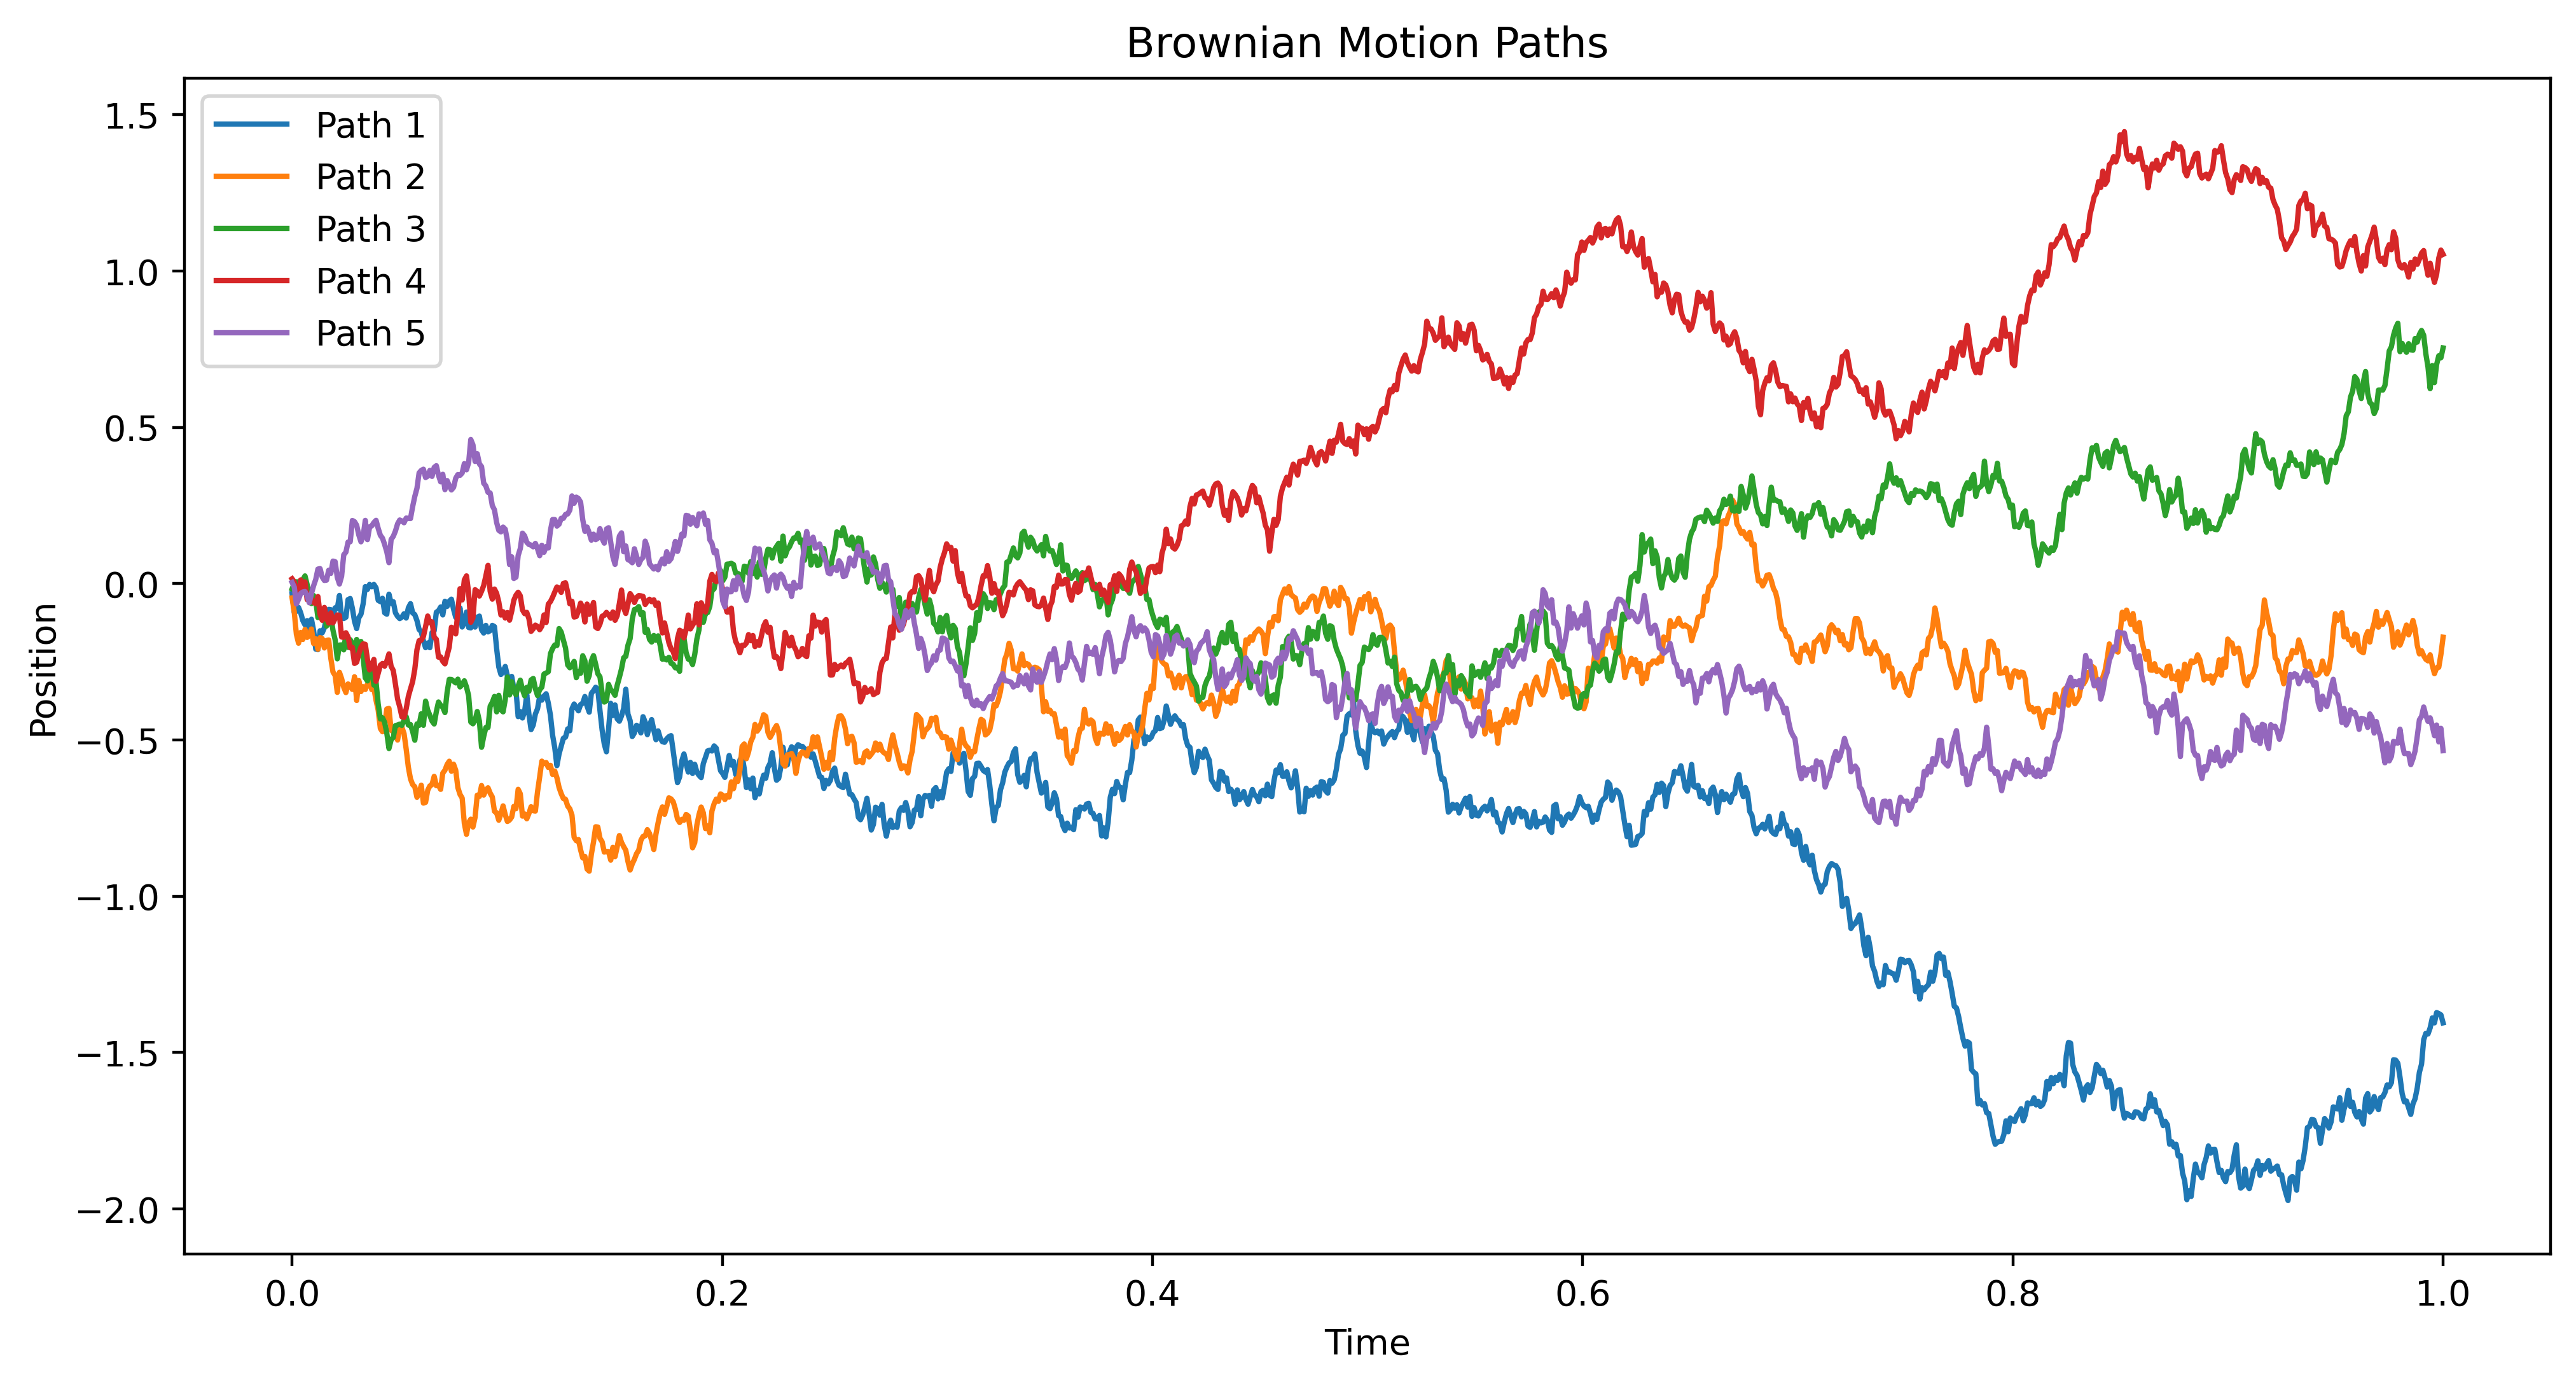
\includegraphics[width=.47\textwidth]{figures/fig1.png}}
    }
    \subfigure[100条布朗运动轨迹]
    {
        {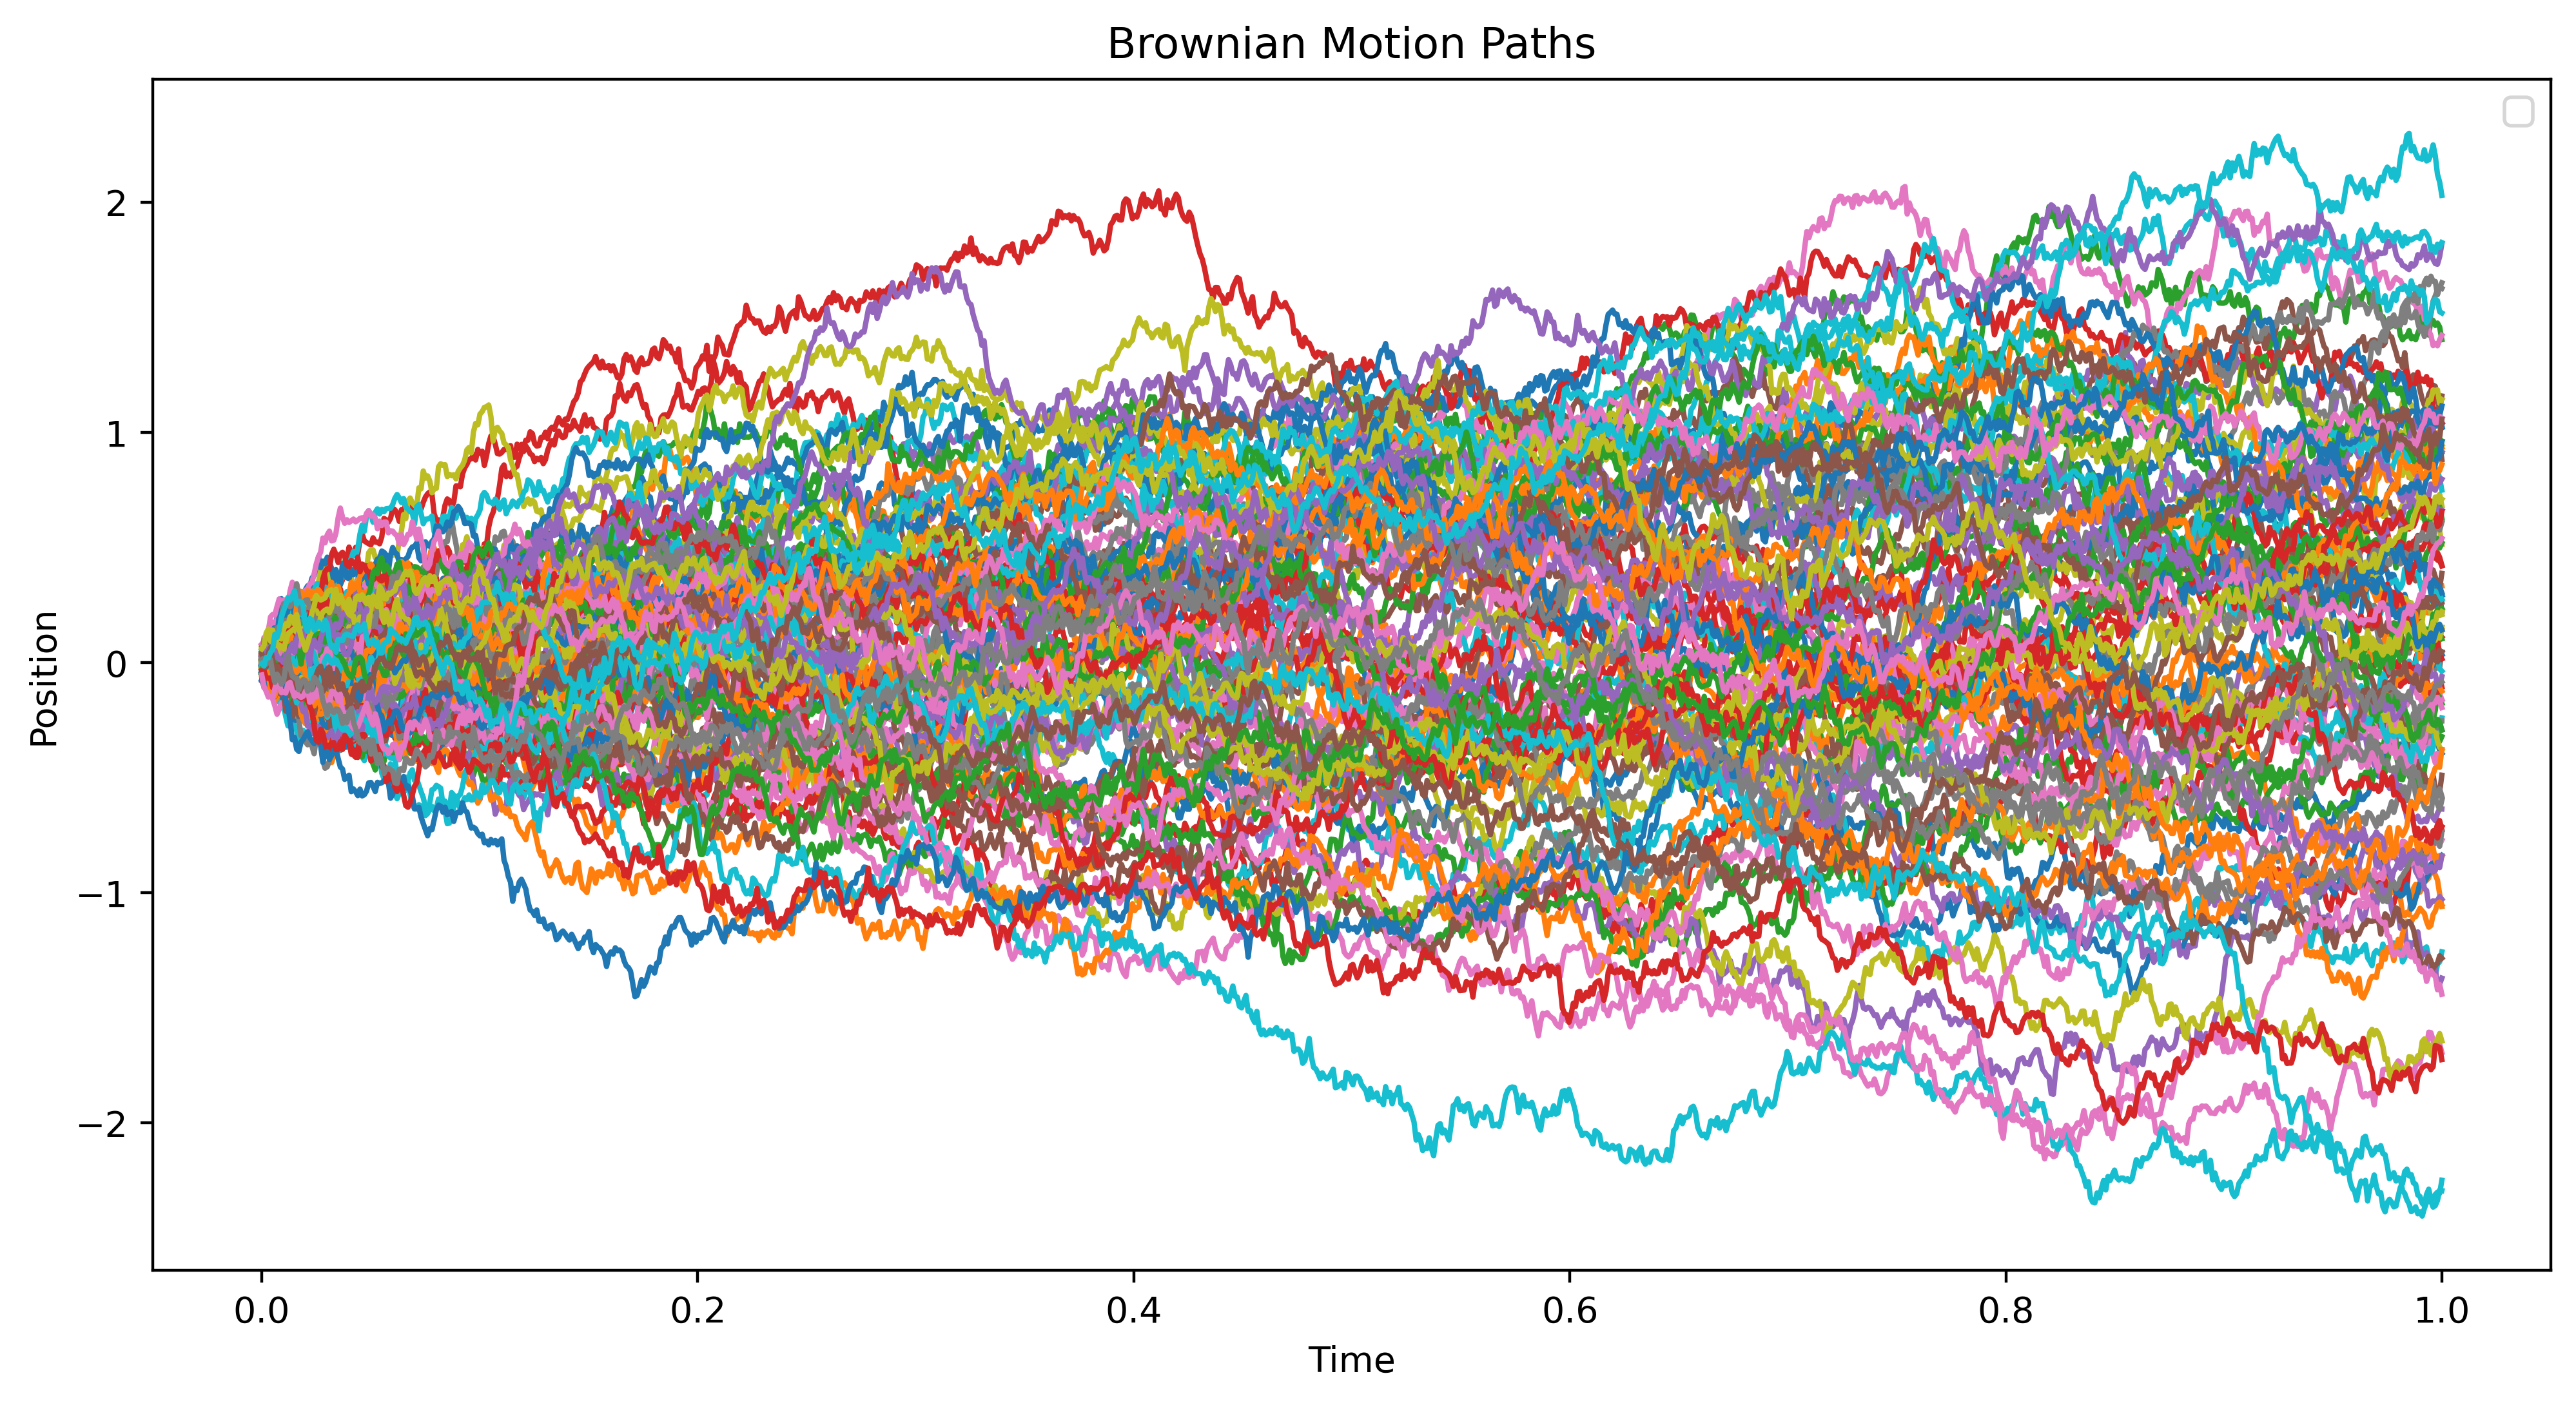
\includegraphics[width=.47\textwidth]{figures/fig2.png}}
    }
\caption{仿真生成多条布朗运动轨道}
\label{fig:brown}
\end{figure}



\subsection{布朗运动一阶变差和二阶变差}
对于布朗运动轨道的每一步,我们计算一阶变差和二阶变差。
\begin{itemize}
    \item 一阶变差:这是轨道上相邻点之间绝对位置变化的累积和。我们首先计算每条轨道上相邻点之间的差异,然后取这些差异的绝对值,最后对这些绝对值进行累积求和。
    \item 二阶变差:这是轨道上相邻点之间位置变化的平方的累积和。我们同样先计算相邻点之间的差异,然后取这些差异的平方,最后对这些平方值进行累积求和。
\end{itemize}
在这两种情况下,我们都是随时间累积这些值,以便能够展示随时间的变化趋势。
\begin{figure}[t]
    \centering
    \subfigure[5条布朗运动1阶变差]
    {
        {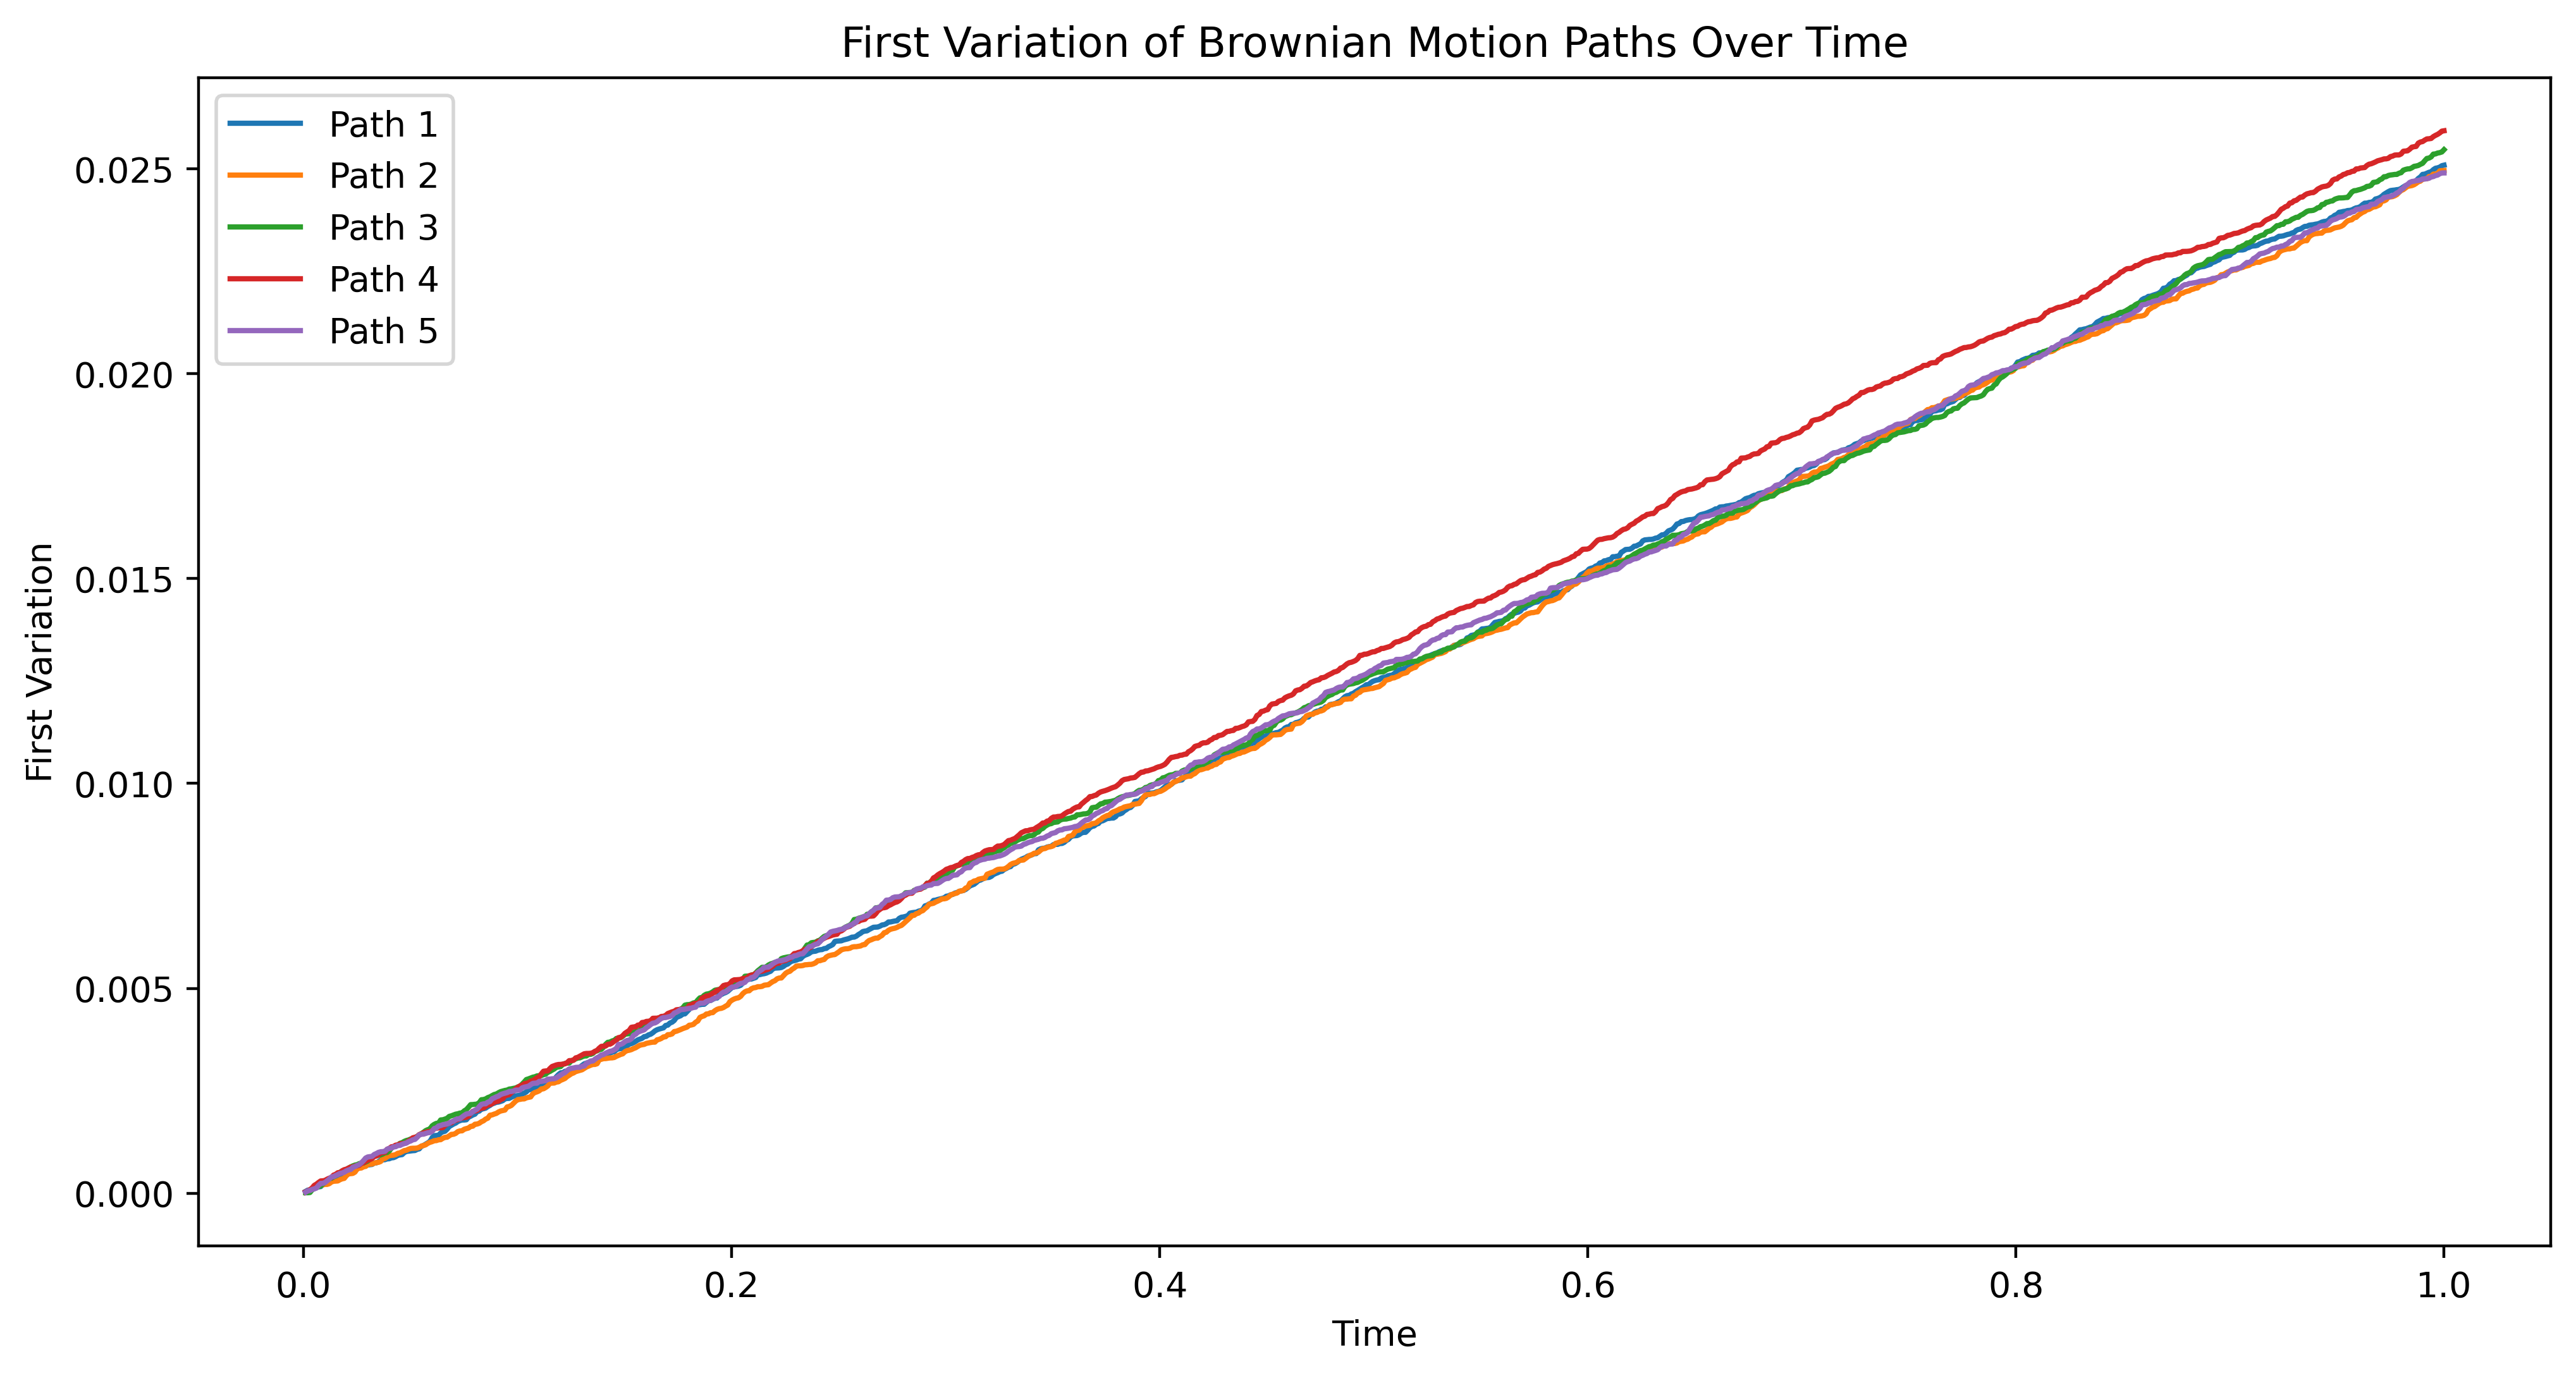
\includegraphics[width=.47\textwidth]{figures/5b1d.png}}
    }
    \subfigure[100条布朗运动1阶变差]
    {
        {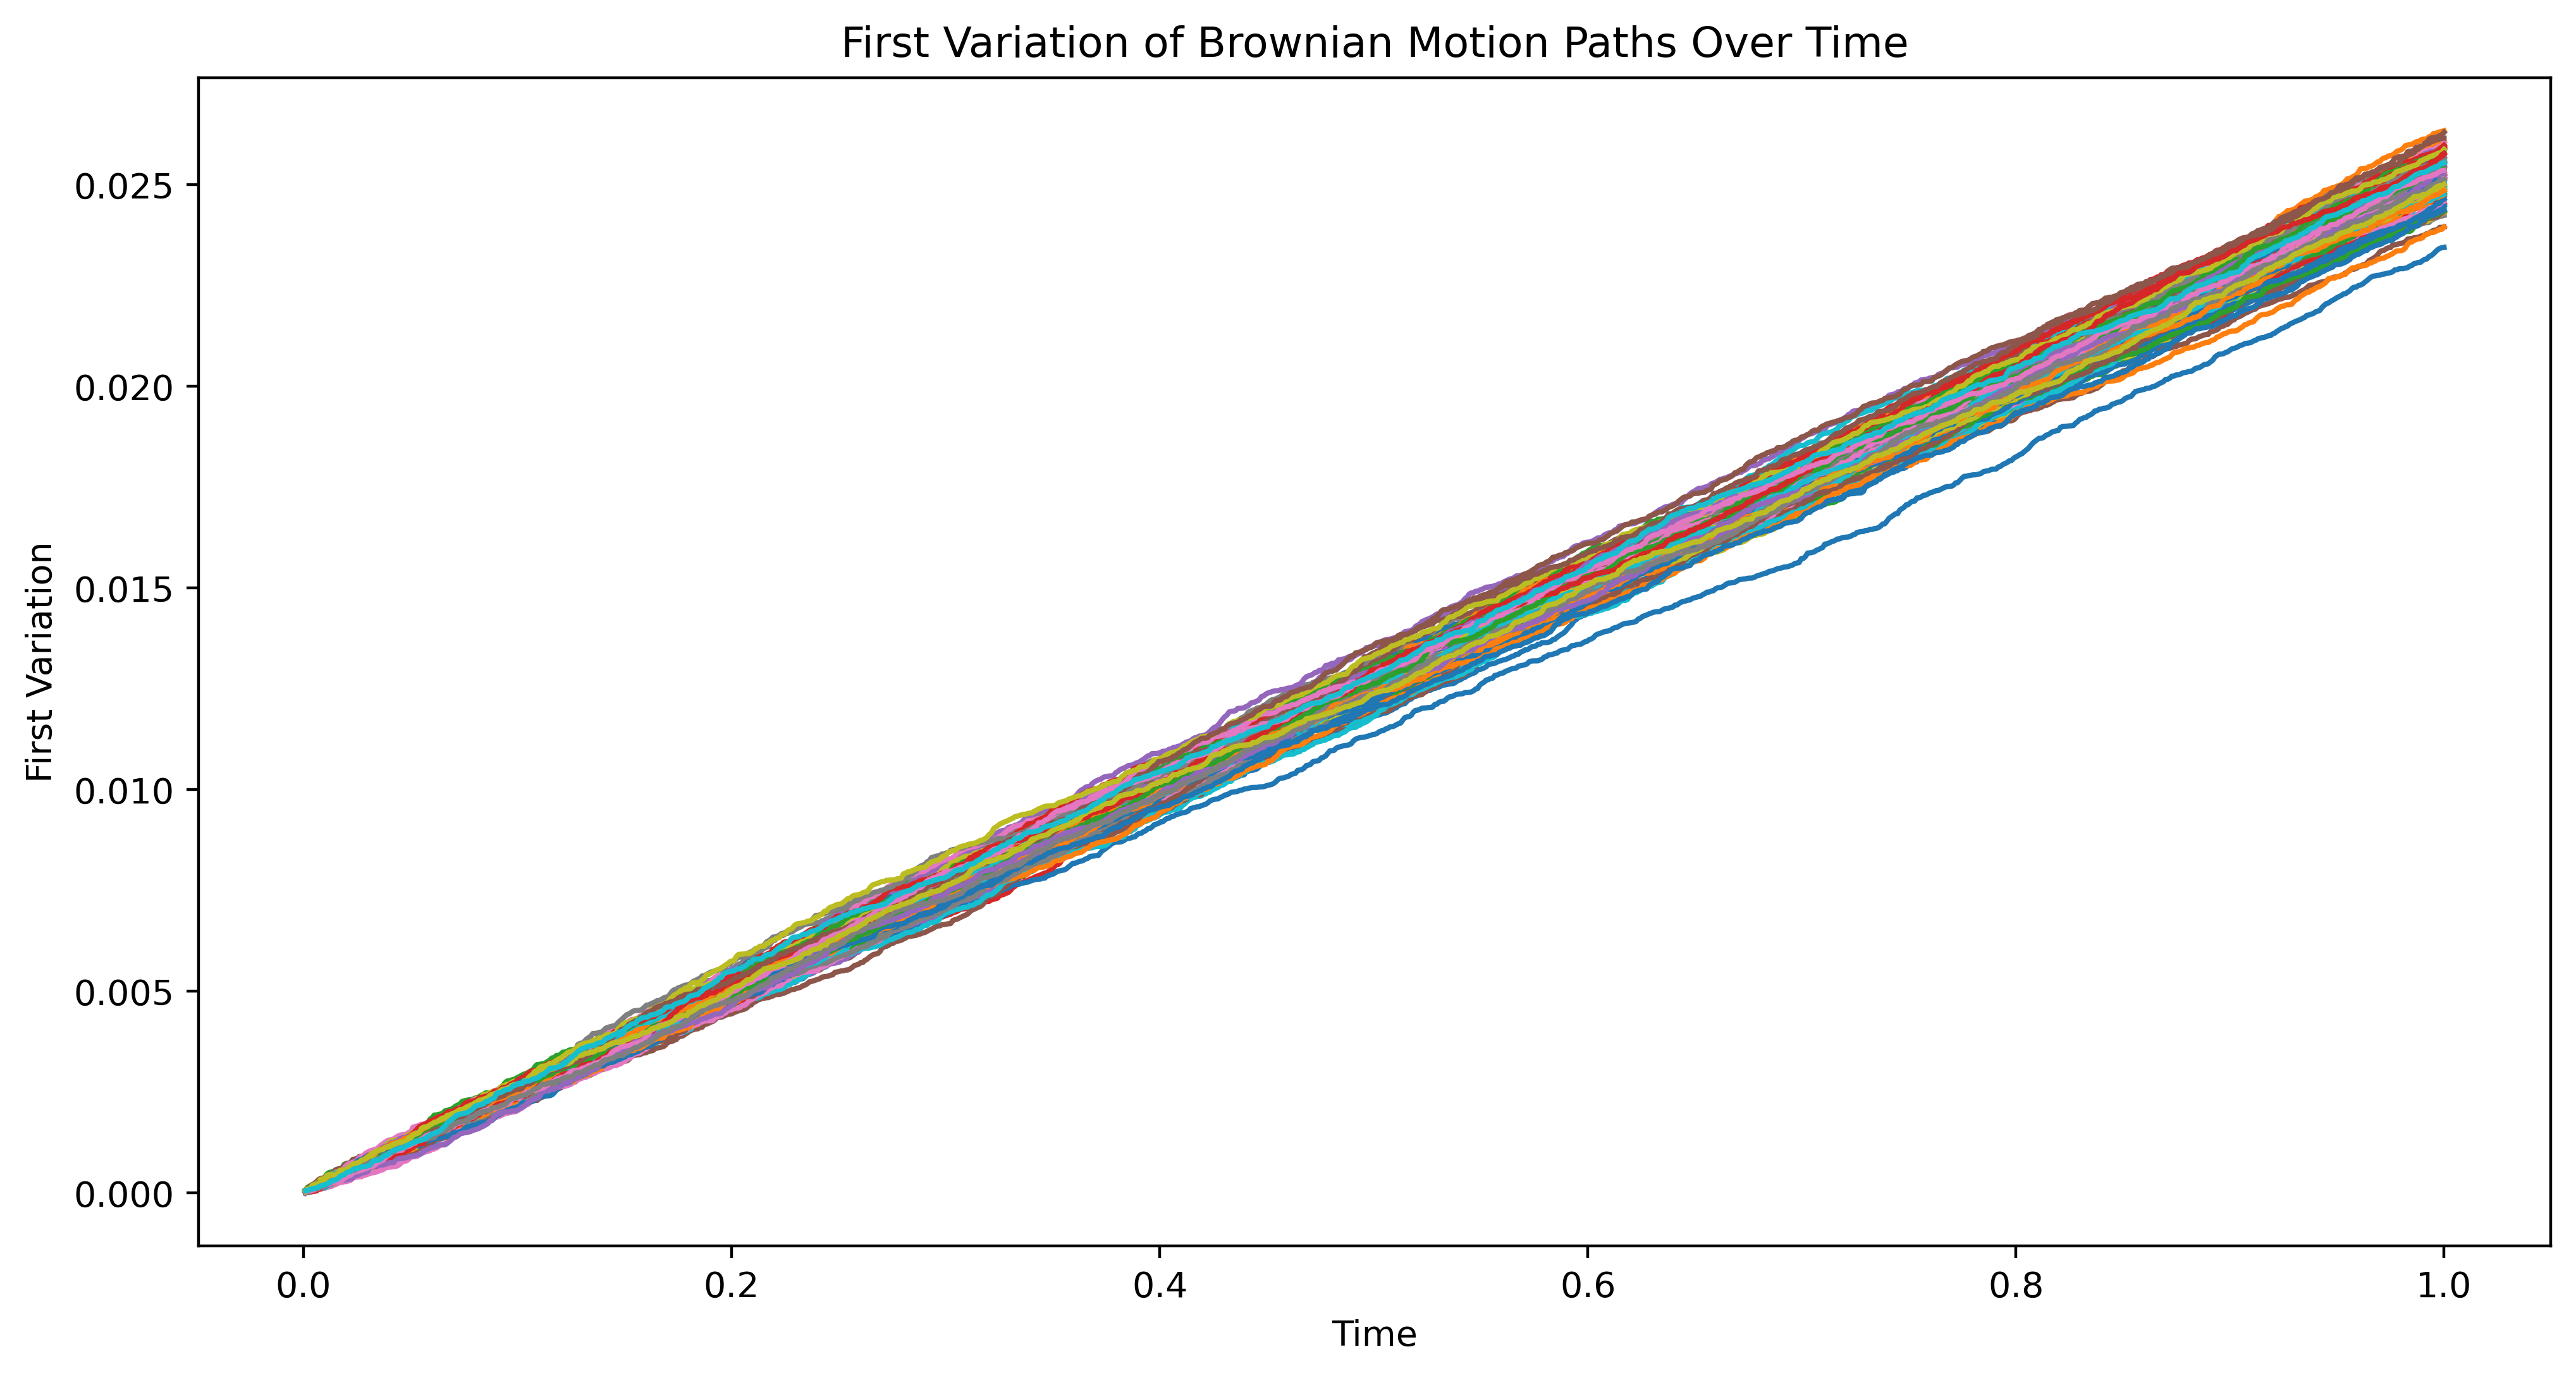
\includegraphics[width=.47\textwidth]{figures/100b1d.png}}
    }
\caption{多条布朗运动轨道1阶变差}
\label{fig:1d}
\end{figure}
\begin{figure}[t]
    \centering
    \subfigure[5条布朗运动2阶变差]
    {
        {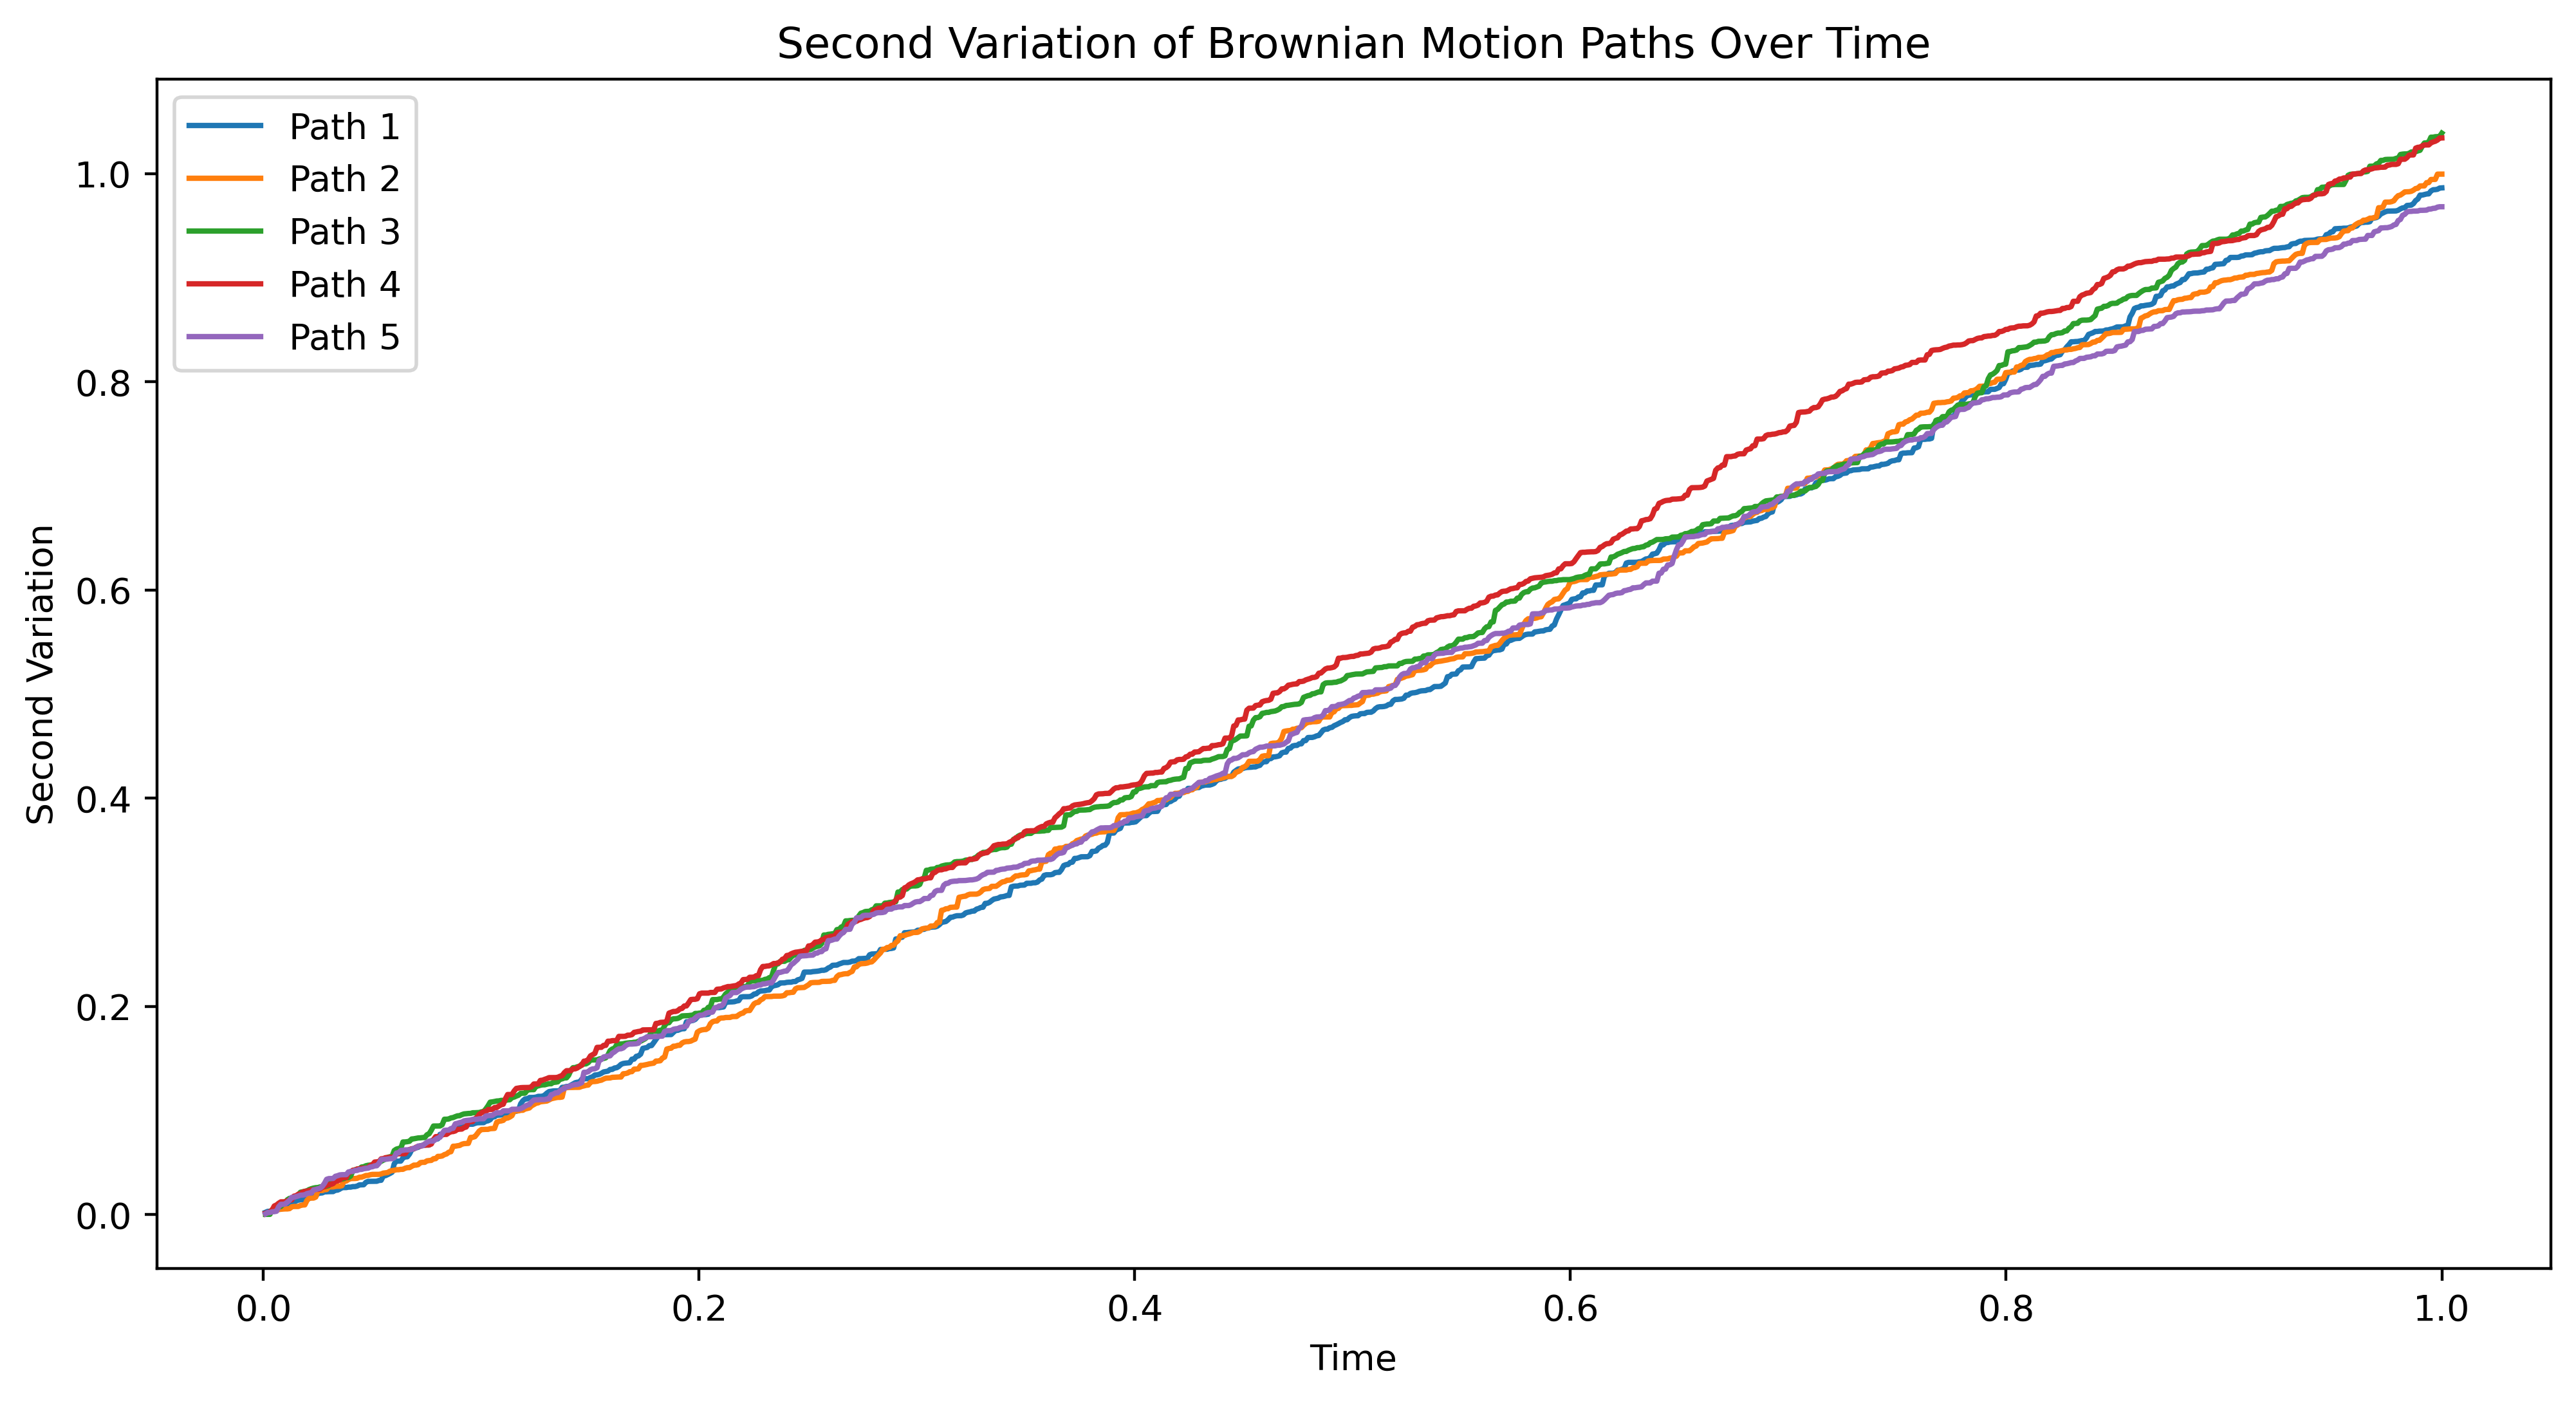
\includegraphics[width=.47\textwidth]{figures/5b2d.png}}
    }
    \subfigure[100条布朗运动2阶变差]
    {
        {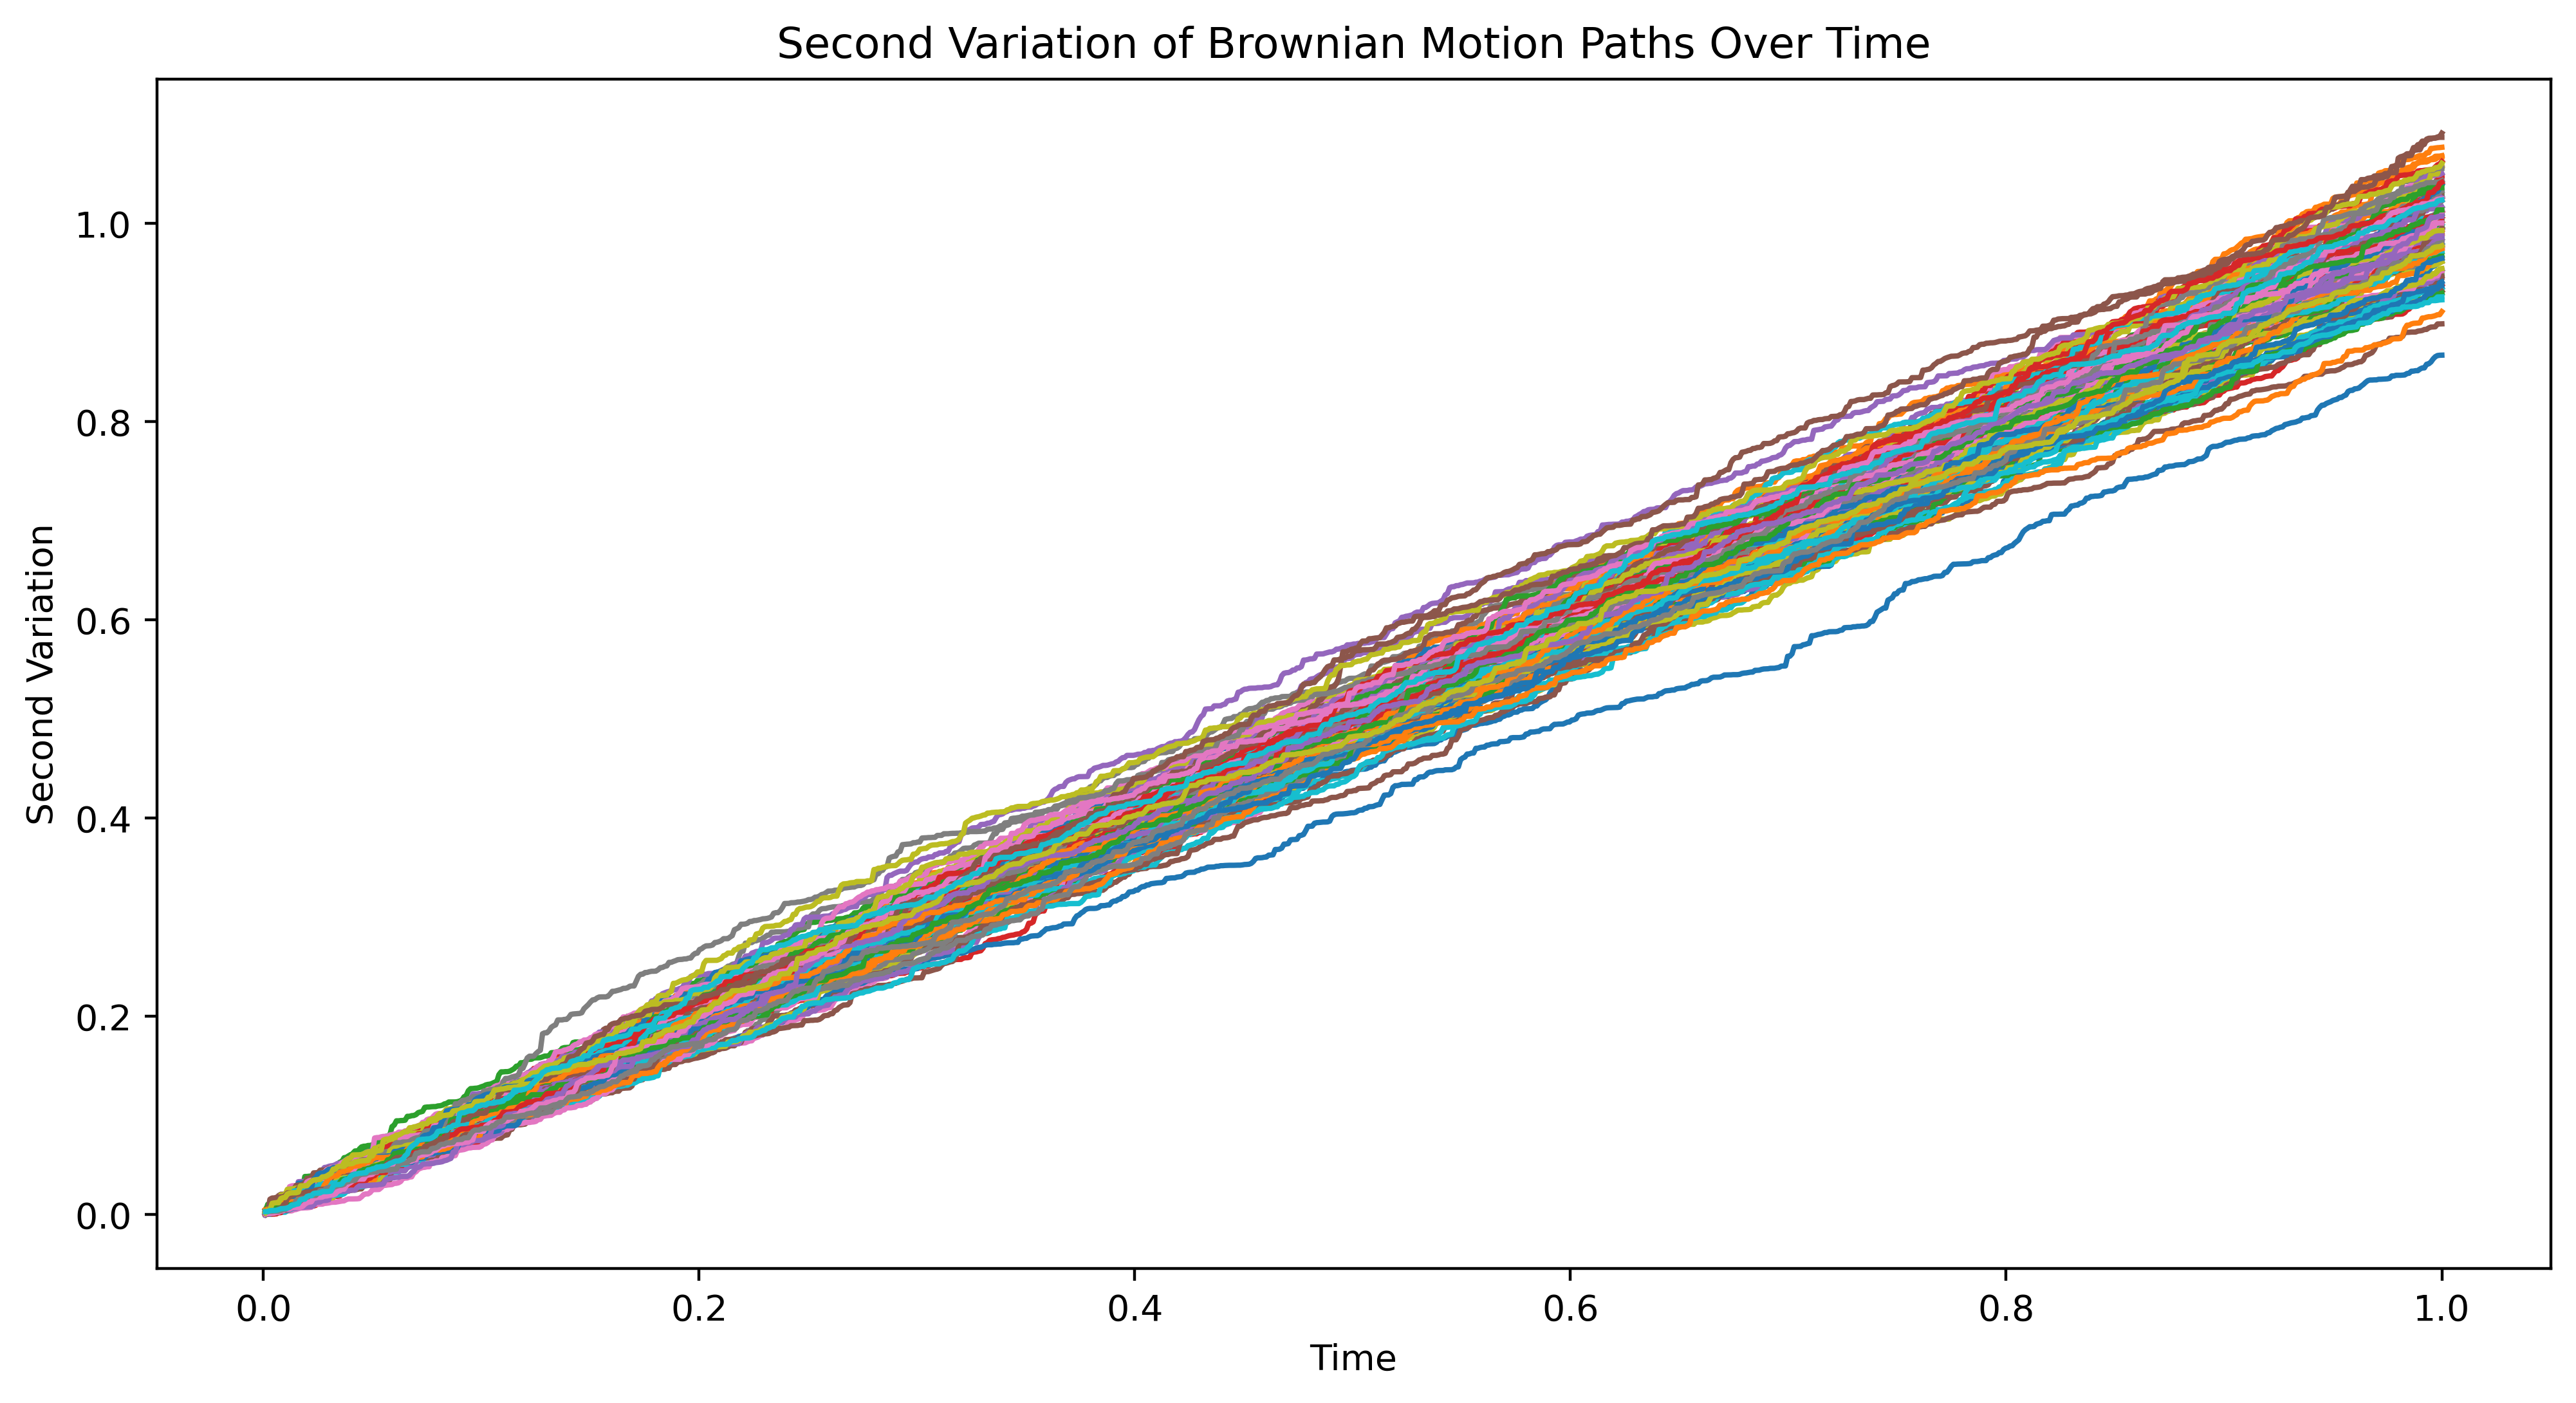
\includegraphics[width=.47\textwidth]{figures/100b2d.png}}
    }
\caption{多条布朗运动轨道2阶变差}
\label{fig:2d}
\end{figure}
尽管布朗运动的轨道本身呈现出高度的随机性和独特性,每条轨道(图\ref{fig:brown})看起来都各不相同,但是当我们观察这些轨道的一阶变差(图\ref{fig:1d})和二阶变差(图\ref{fig:2d})时,会发现一个有趣的现象:尽管原始轨道本身极为不规则,它们的变差轨道却展现出一种惊人的一致性,呈现出近似直线的趋势。

这种现象反映了布朗运动作为随机过程的内在特性。布朗运动的一阶变差基本上代表了路径的累积“移动距离”,随着时间的推移,这种累积效应即使在不断变化的路径中也表现出一定的规律性。同样地,二阶变差反映了路径的累积“波动大小”,它随时间的增长而增长,几乎呈现出线性的增长趋势。



\section{SDE数值模拟}

我们观察研究问题二中的随机微分方程 (SDE) 的形式:

\begin{equation}
   X_t = \alpha (v - X_t) dt + \sigma dB_t, \quad X_0 = x_0 
\end{equation} 
我们可以发现,这个方程是一个线性随机微分方程,其中 $\alpha$, $v$, $\sigma$是常数,$B_t$是一个标准布朗运动。求解这类方程通常需要使用随机过程和随机微积分的技术。对于上述方程,其解 $X_t$ 是一个随时间变化的随机过程,不能用封闭形式的表达式简单表示。然而,它可以通过数值方法(如Euler-Maruyama方法)进行模拟。

这个方程是一个典型的Ornstein-Uhlenbeck过程,用于描述具有均值回归特性的随机过程。在这个过程中,$X_t$趋向于长期均值$v$,而这种趋势受到随机波动(由$\sigma$ $dB_t$ 部分引入)的影响。

要数值模拟这个随机微分方程,可以使用Euler-Maruyama方法,这是一种用于数值求解SDE的简单而有效的方法。基本思想是将时间分割成小的间隔,并在每个间隔上近似随机微分方程。

对于每个时间步 \( \Delta t \),模拟公式可以表示为:

\[ X_{t+\Delta t} = X_t + \alpha(v - X_t)\Delta t + \sigma \sqrt{\Delta t} \, \epsilon_t \]

其中 \( \epsilon_t \) 是一个从标准正态分布中抽取的随机样本。

通过从初始值 \( X_0 = x_0 \) 开始,重复应用这个公式,可以生成 \( X_t \) 的近似路径。这种方法在小的时间步长下通常非常有效,但需要注意,由于是随机模拟,每次运行都可能产生不同的结果。


在这些公式中,\(dX_t\) 表示随机过程 \(X_t\) 的微分,\(\alpha\) 和 \(\sigma\) 是常数参数,\(v\) 是长期均值,\(dB_t\) 是标准布朗运动的增量,\(X_0 = x_0\) 是初始条件。Euler-Maruyama 方法使用时间间隔 \(\Delta t\) 和随机项 \(\epsilon_t\)(通常从标准正态分布中抽取)来近似这个过程。

\begin{figure}[t]
    \centering
    \subfigure[模拟$X_t$轨道]
    {
        {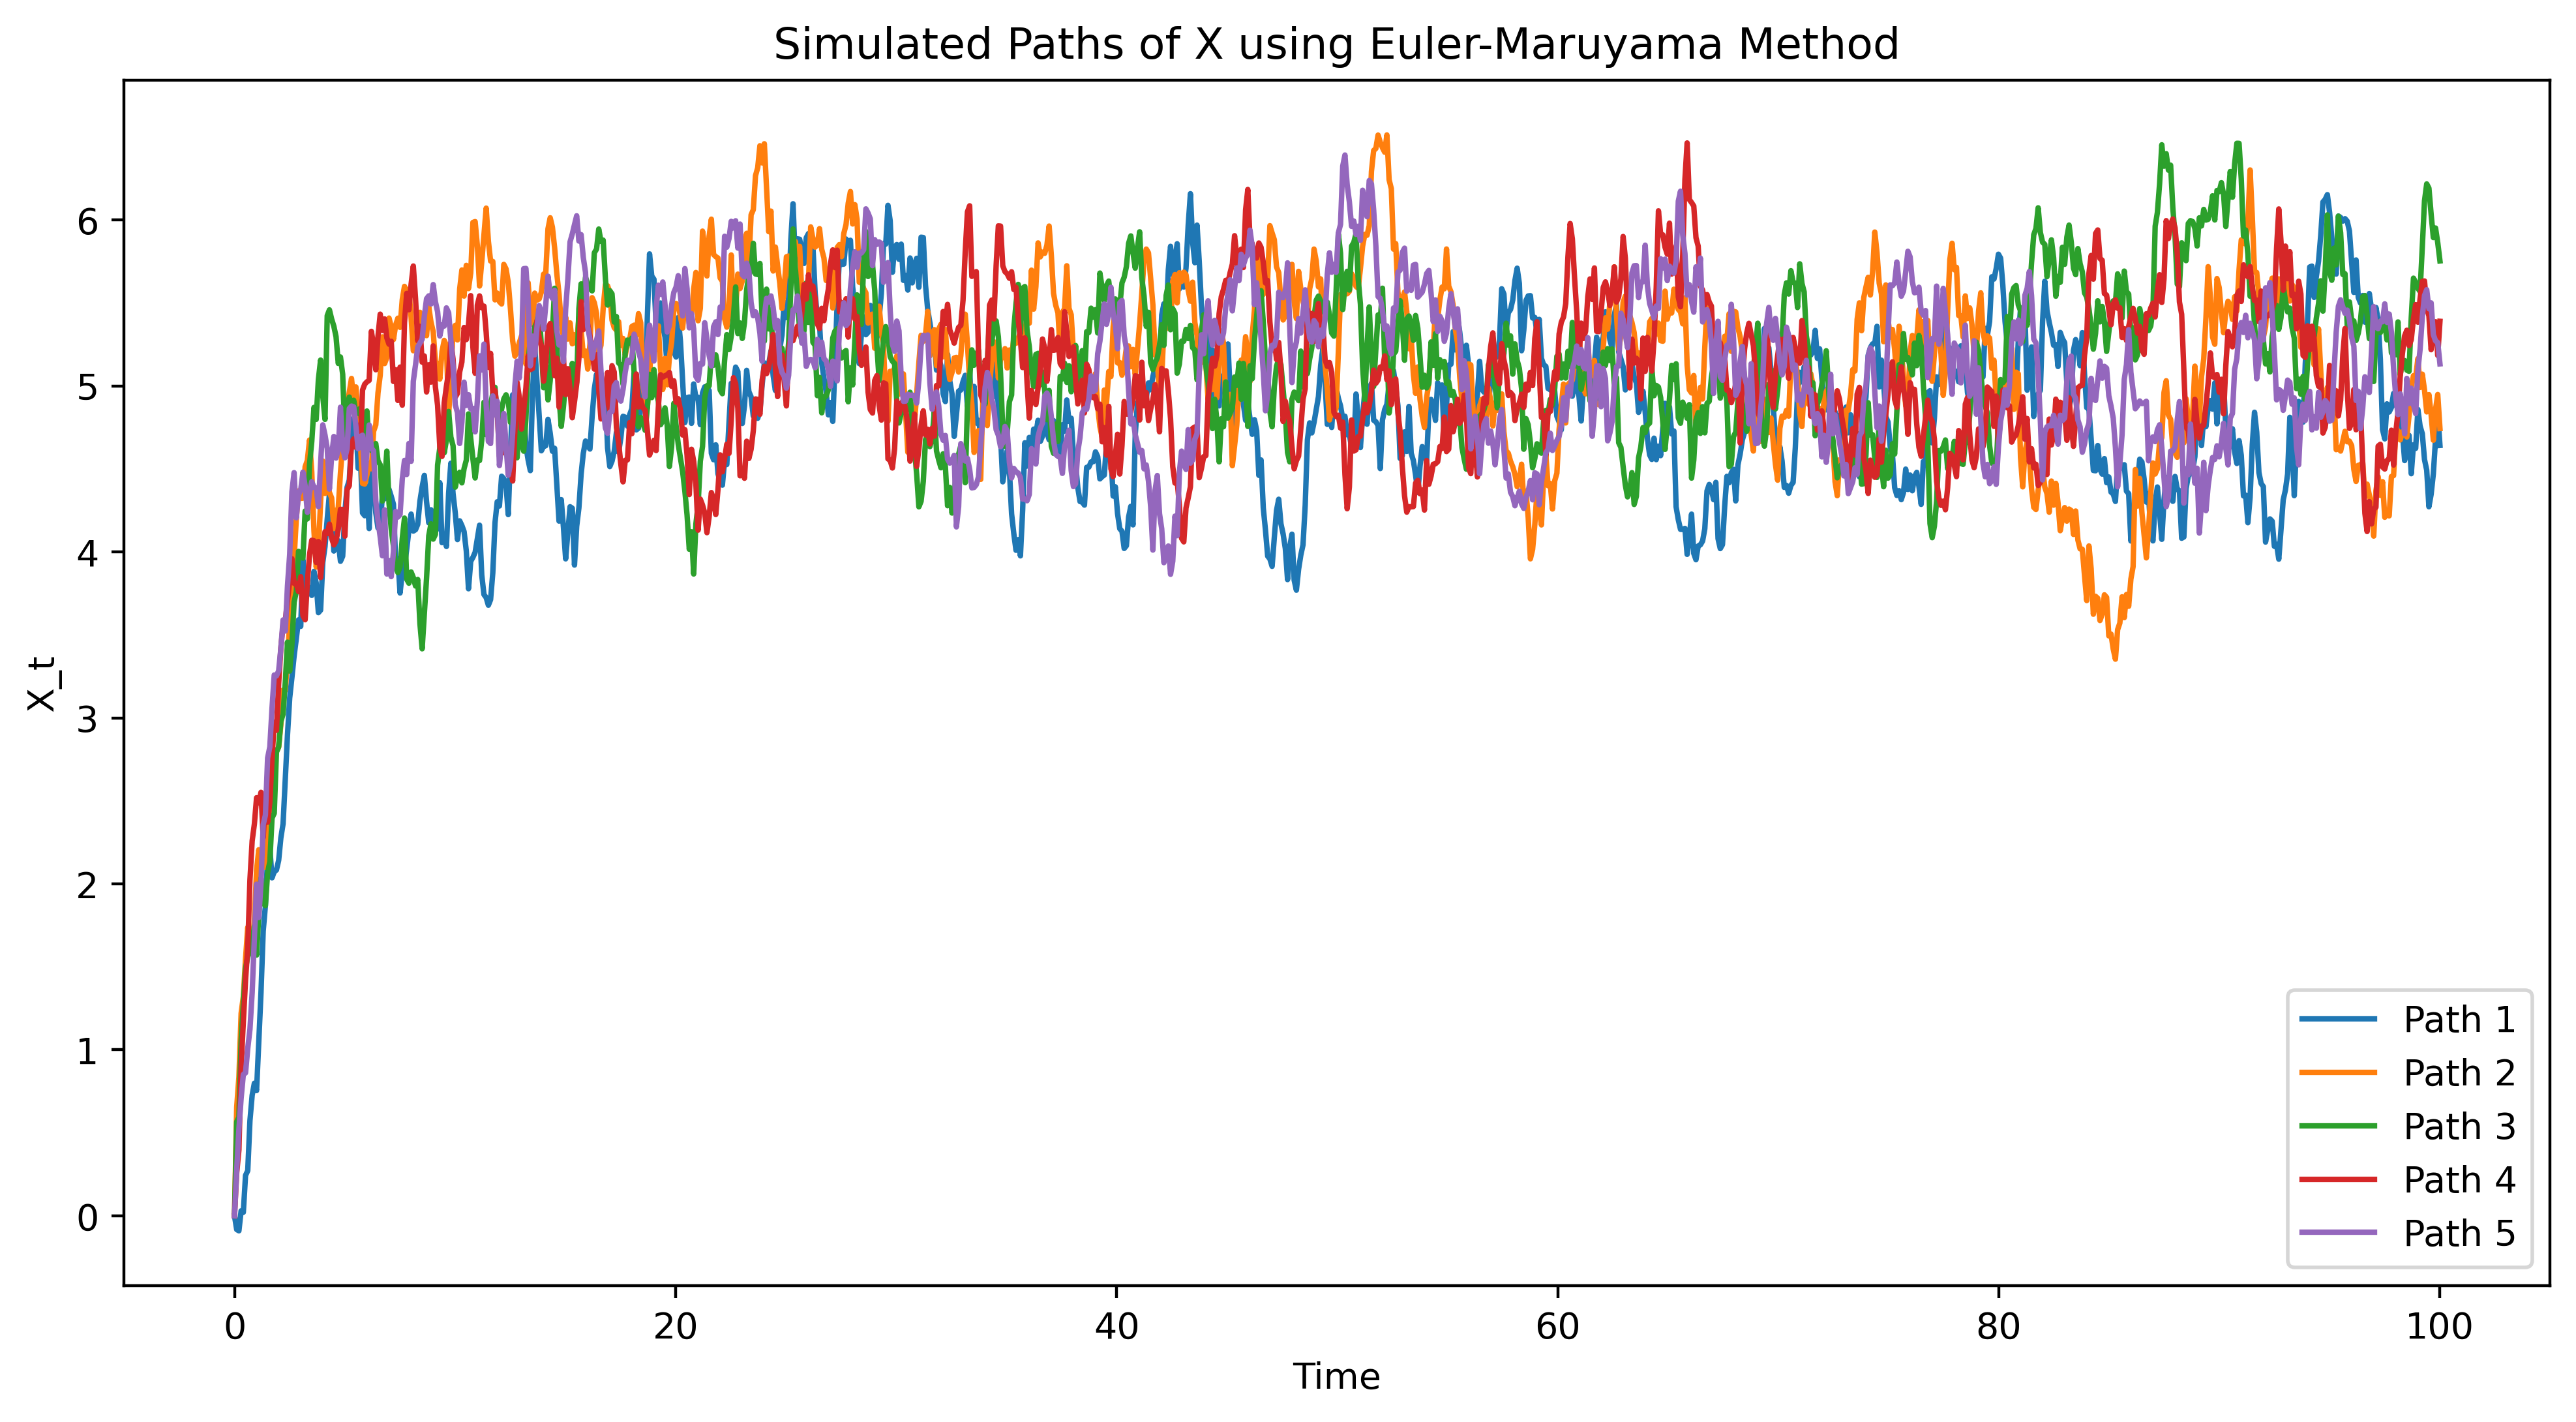
\includegraphics[width=.47\textwidth]{figures/EM1.png}}
    }
    \subfigure[模拟$X_t$轨道2阶变差]
    {
        {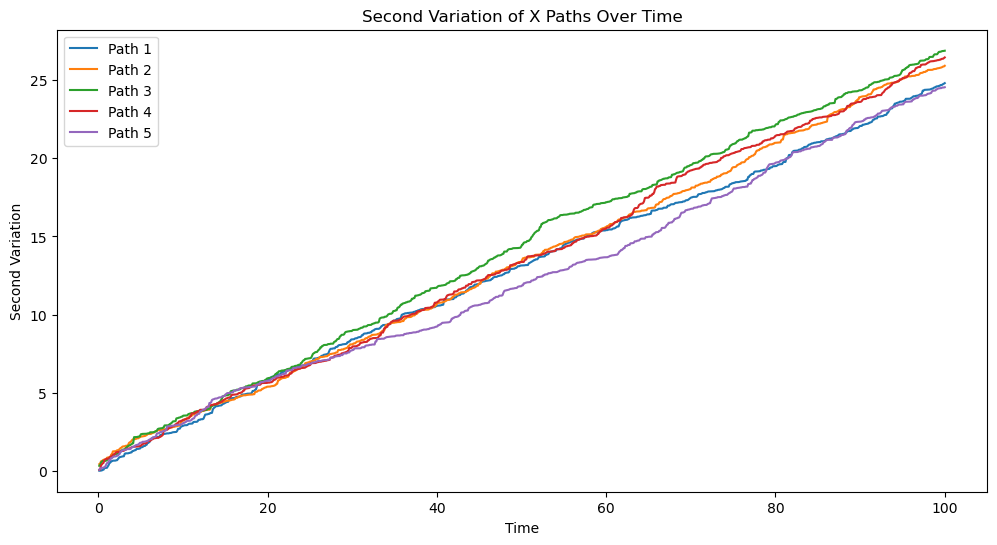
\includegraphics[width=.47\textwidth]{figures/EM2d.png}}
    }
\caption{$\alpha=0.5$, $v=5$,$sigma=0.5$, $x_0=0$}
\label{fig:EM1}
\end{figure}
\begin{figure}[t]
    \centering
    \subfigure[模拟$X_t$轨道]
    {
        {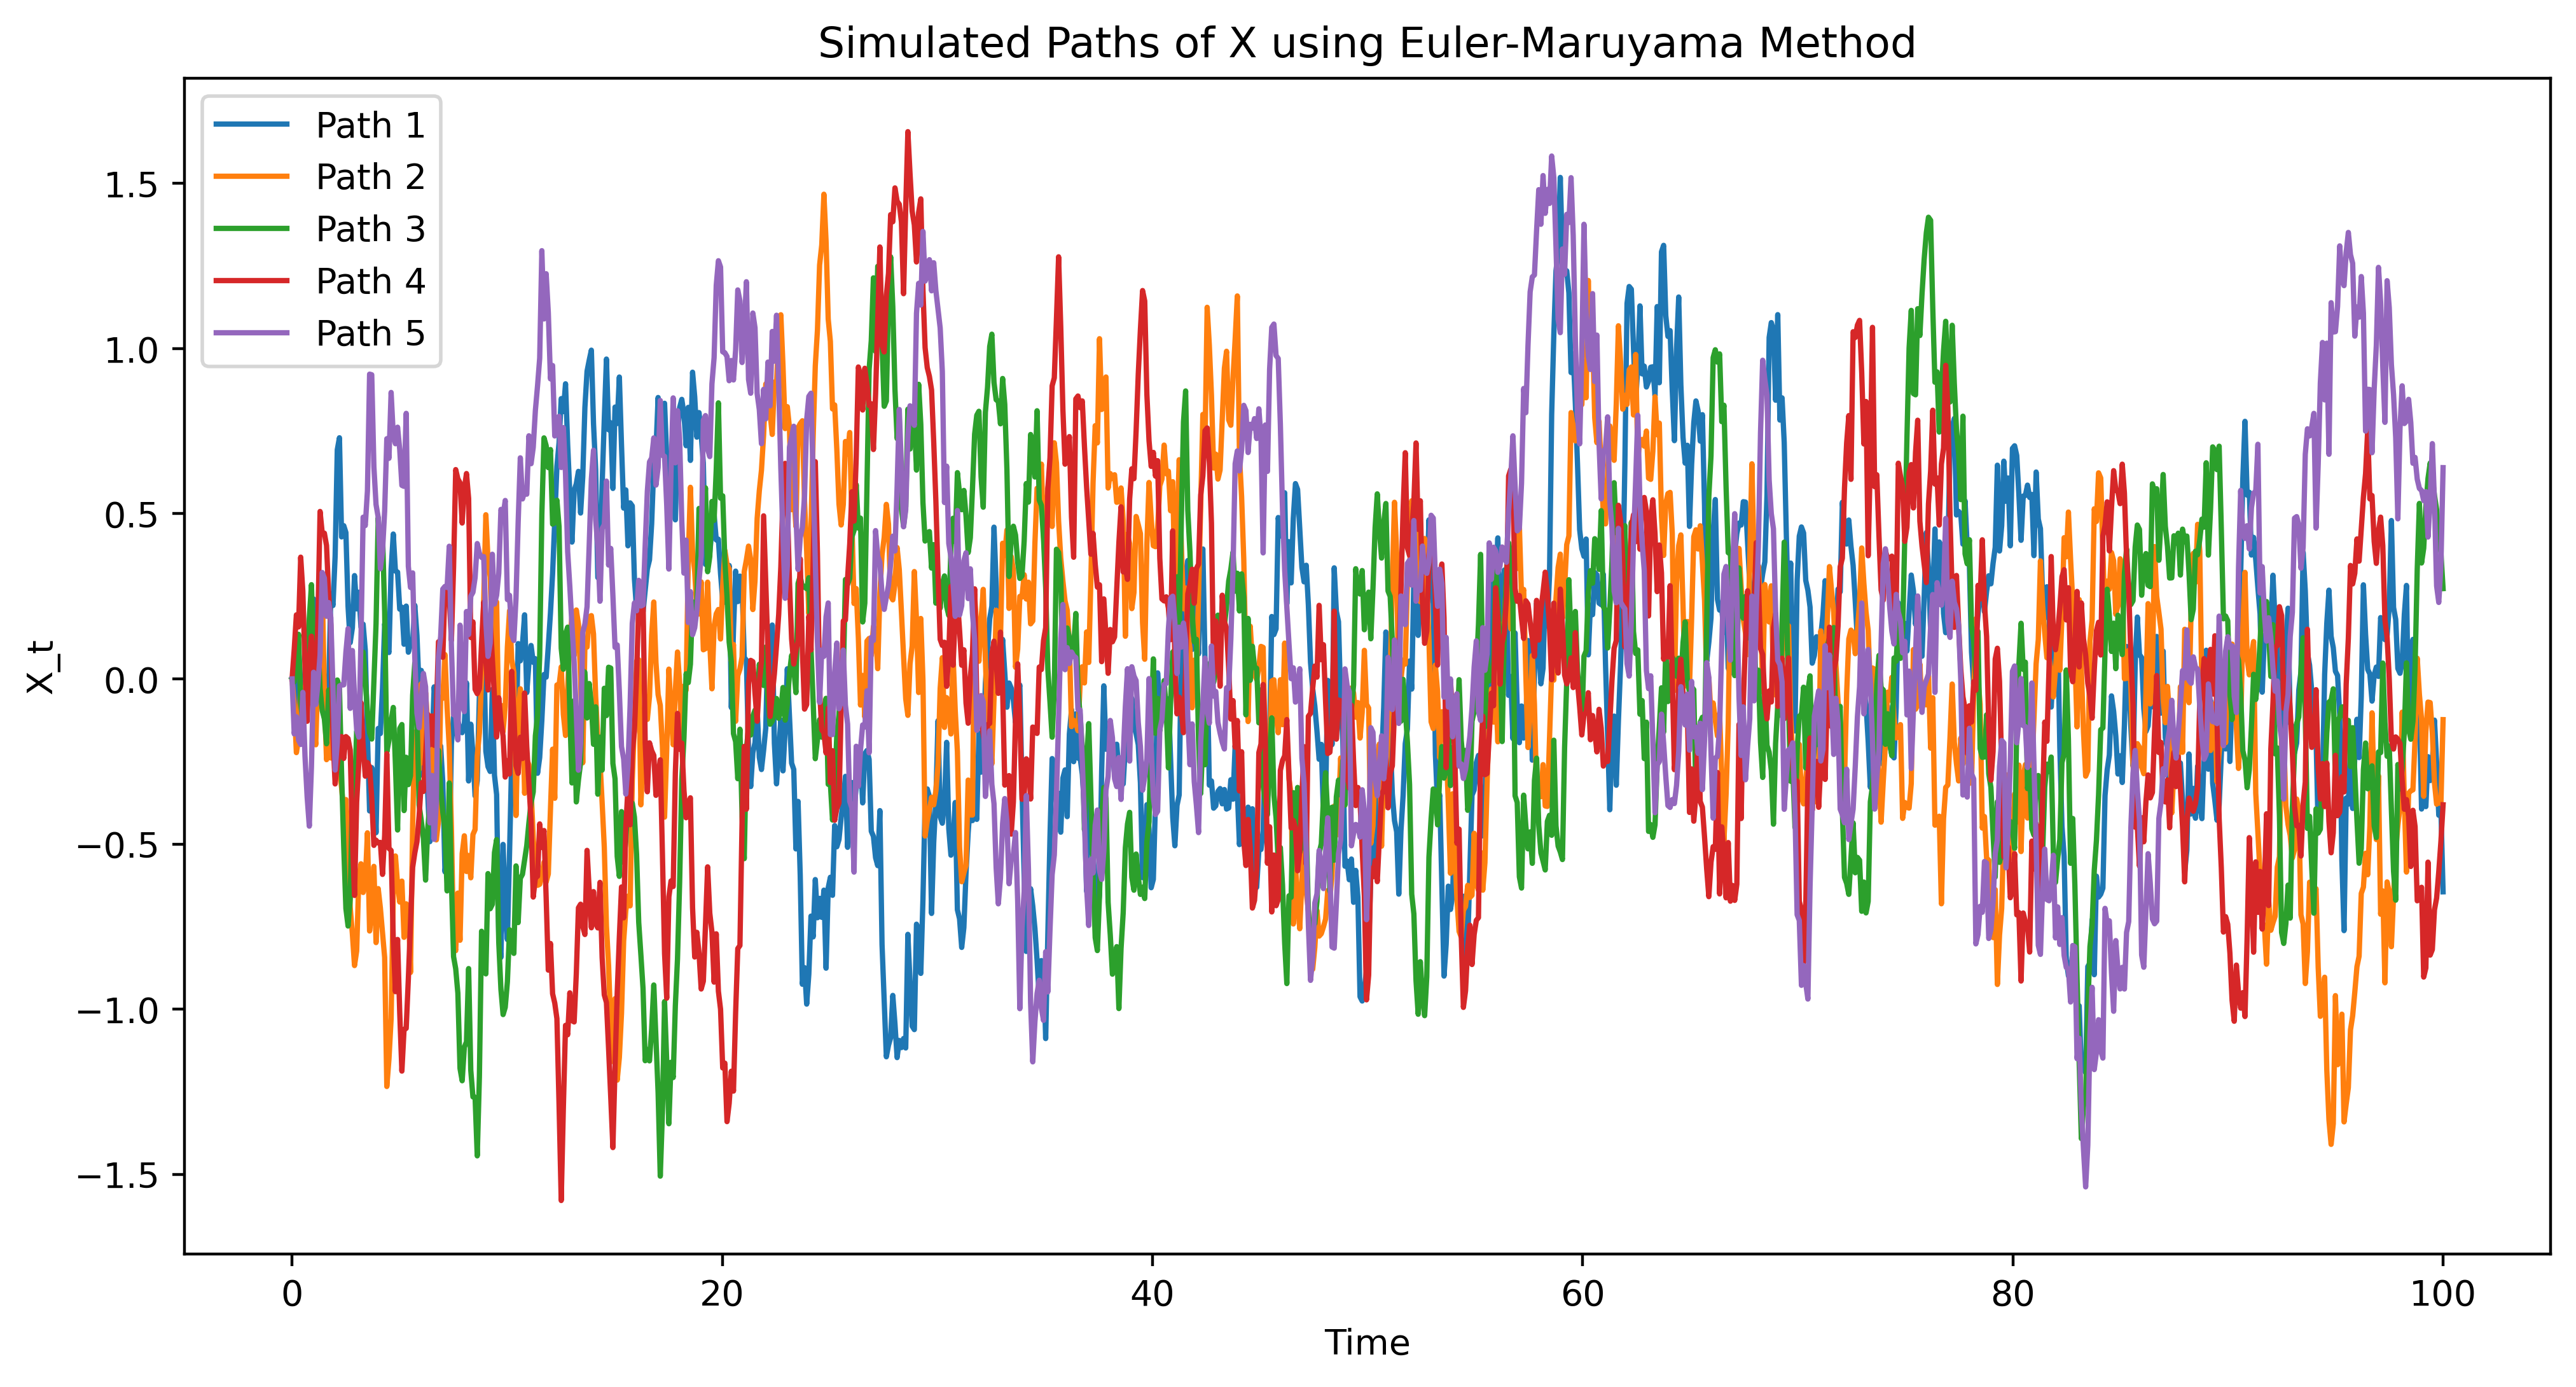
\includegraphics[width=.47\textwidth]{figures/EM2.png}}
    }
    \subfigure[模拟$X_t$轨道2阶变差]
    {
        {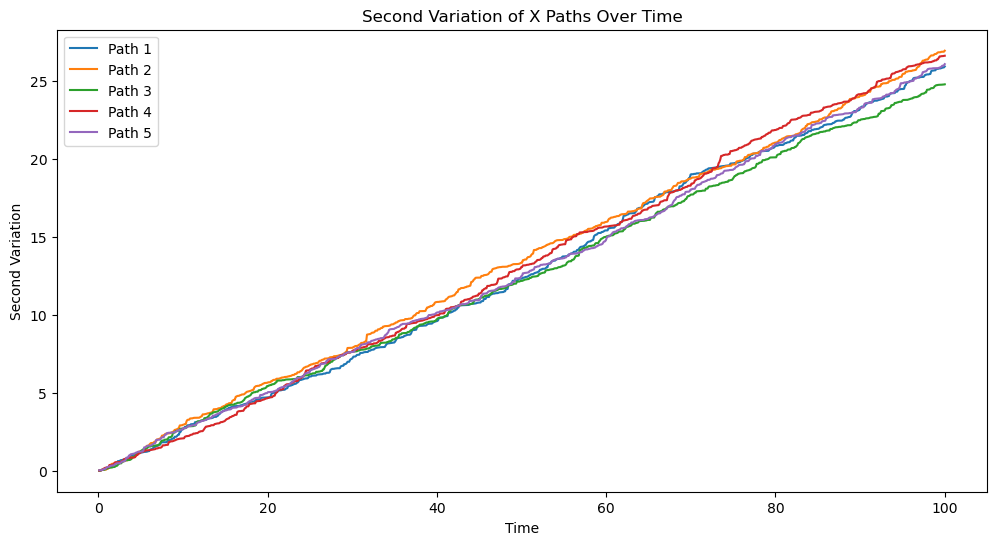
\includegraphics[width=.47\textwidth]{figures/EM22d.png}}
    }
\caption{$\alpha=0.5$, $v=0$,$sigma=0.5$, $x_0=0$}
\label{fig:EM2}
\end{figure}
\begin{figure}[t]
    \centering
    \subfigure[模拟$X_t$轨道]
    {
        {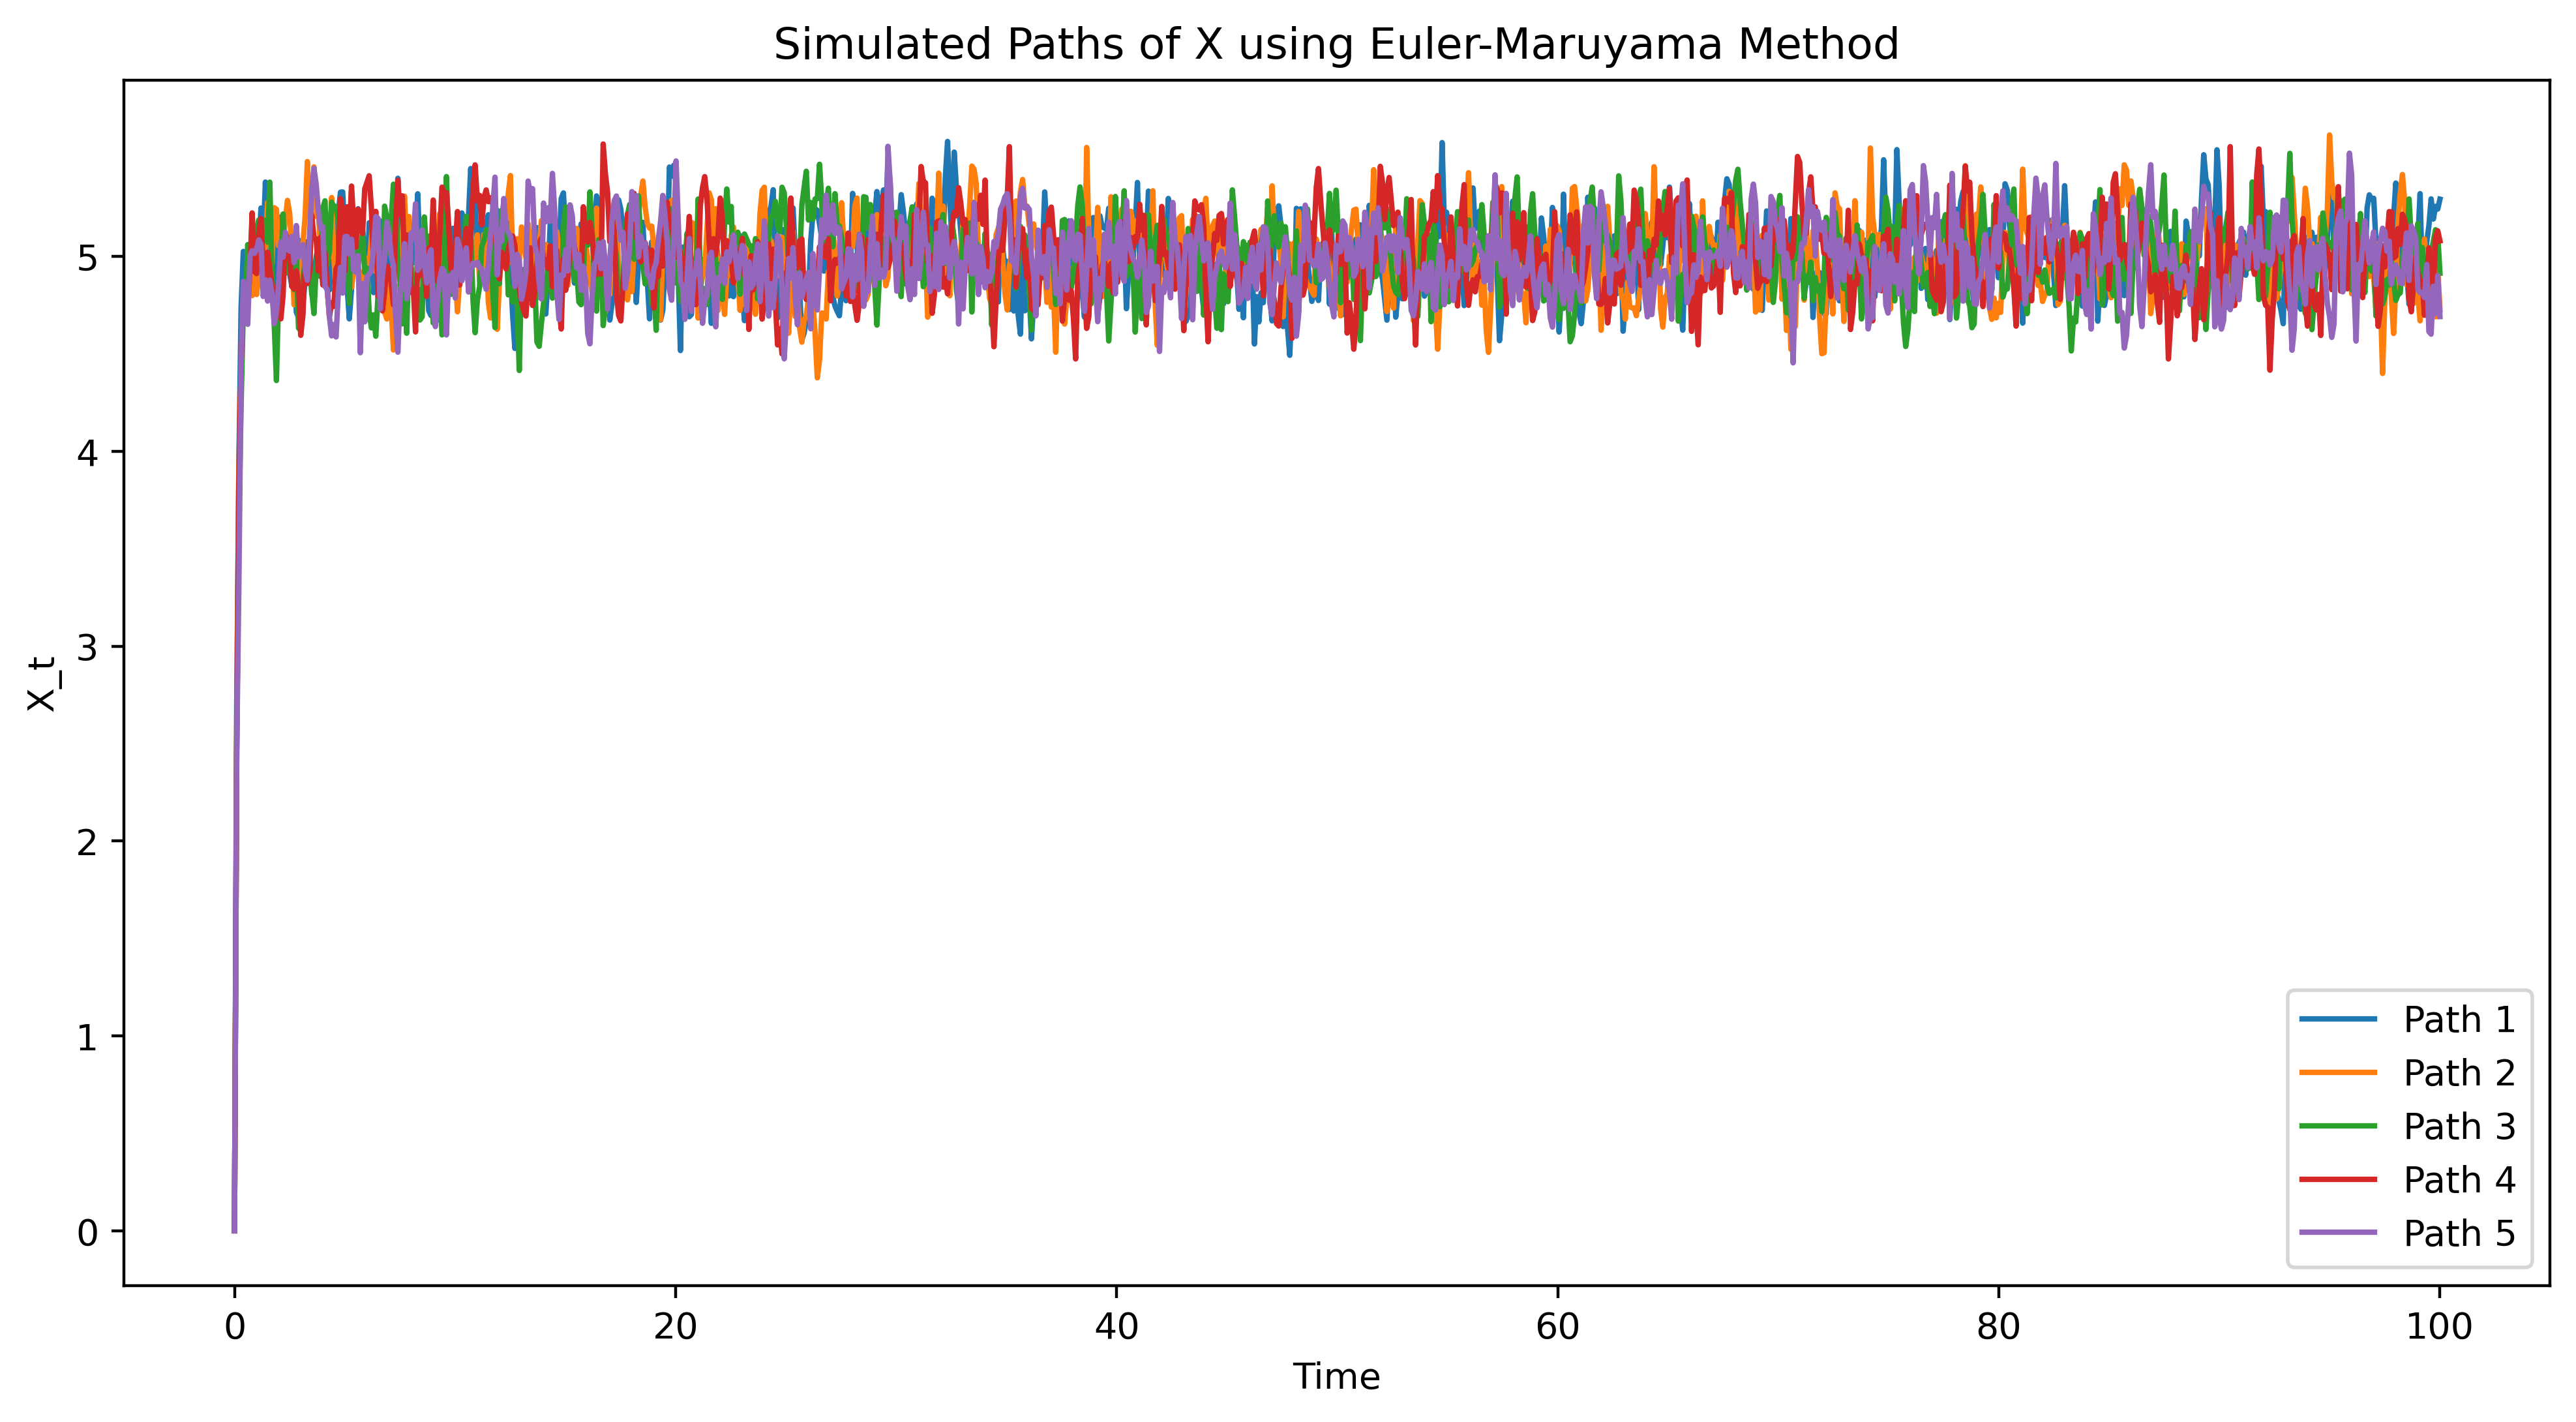
\includegraphics[width=.47\textwidth]{figures/EM3.png}}
    }
    \subfigure[模拟$X_t$轨道2阶变差]
    {
        {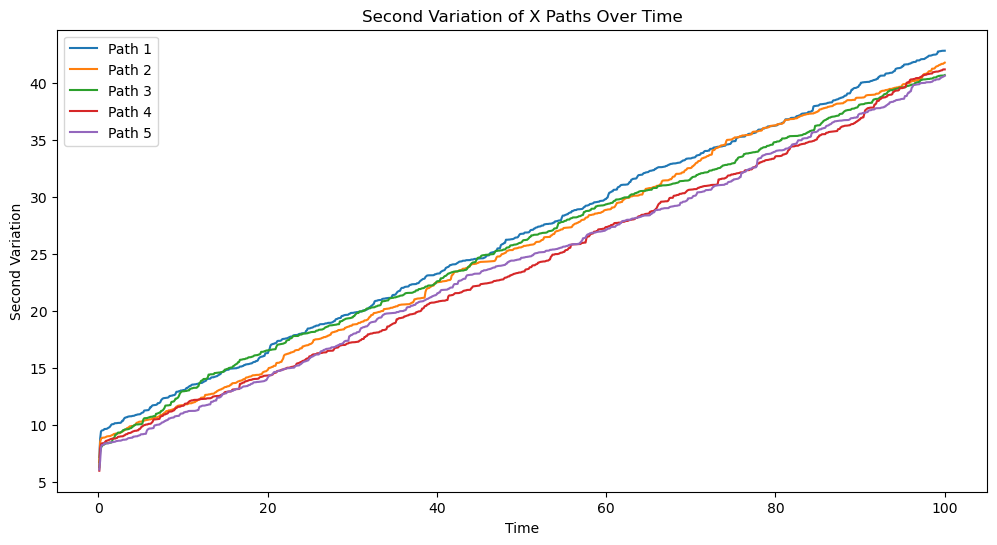
\includegraphics[width=.47\textwidth]{figures/EM32d.png}}
    }
\caption{$\alpha=5$, $v=5$,$sigma=0.5$, $x_0=0$}
\label{fig:EM3}
\end{figure}
\begin{figure}[t]
    \centering
    \subfigure[模拟$X_t$轨道]
    {
        {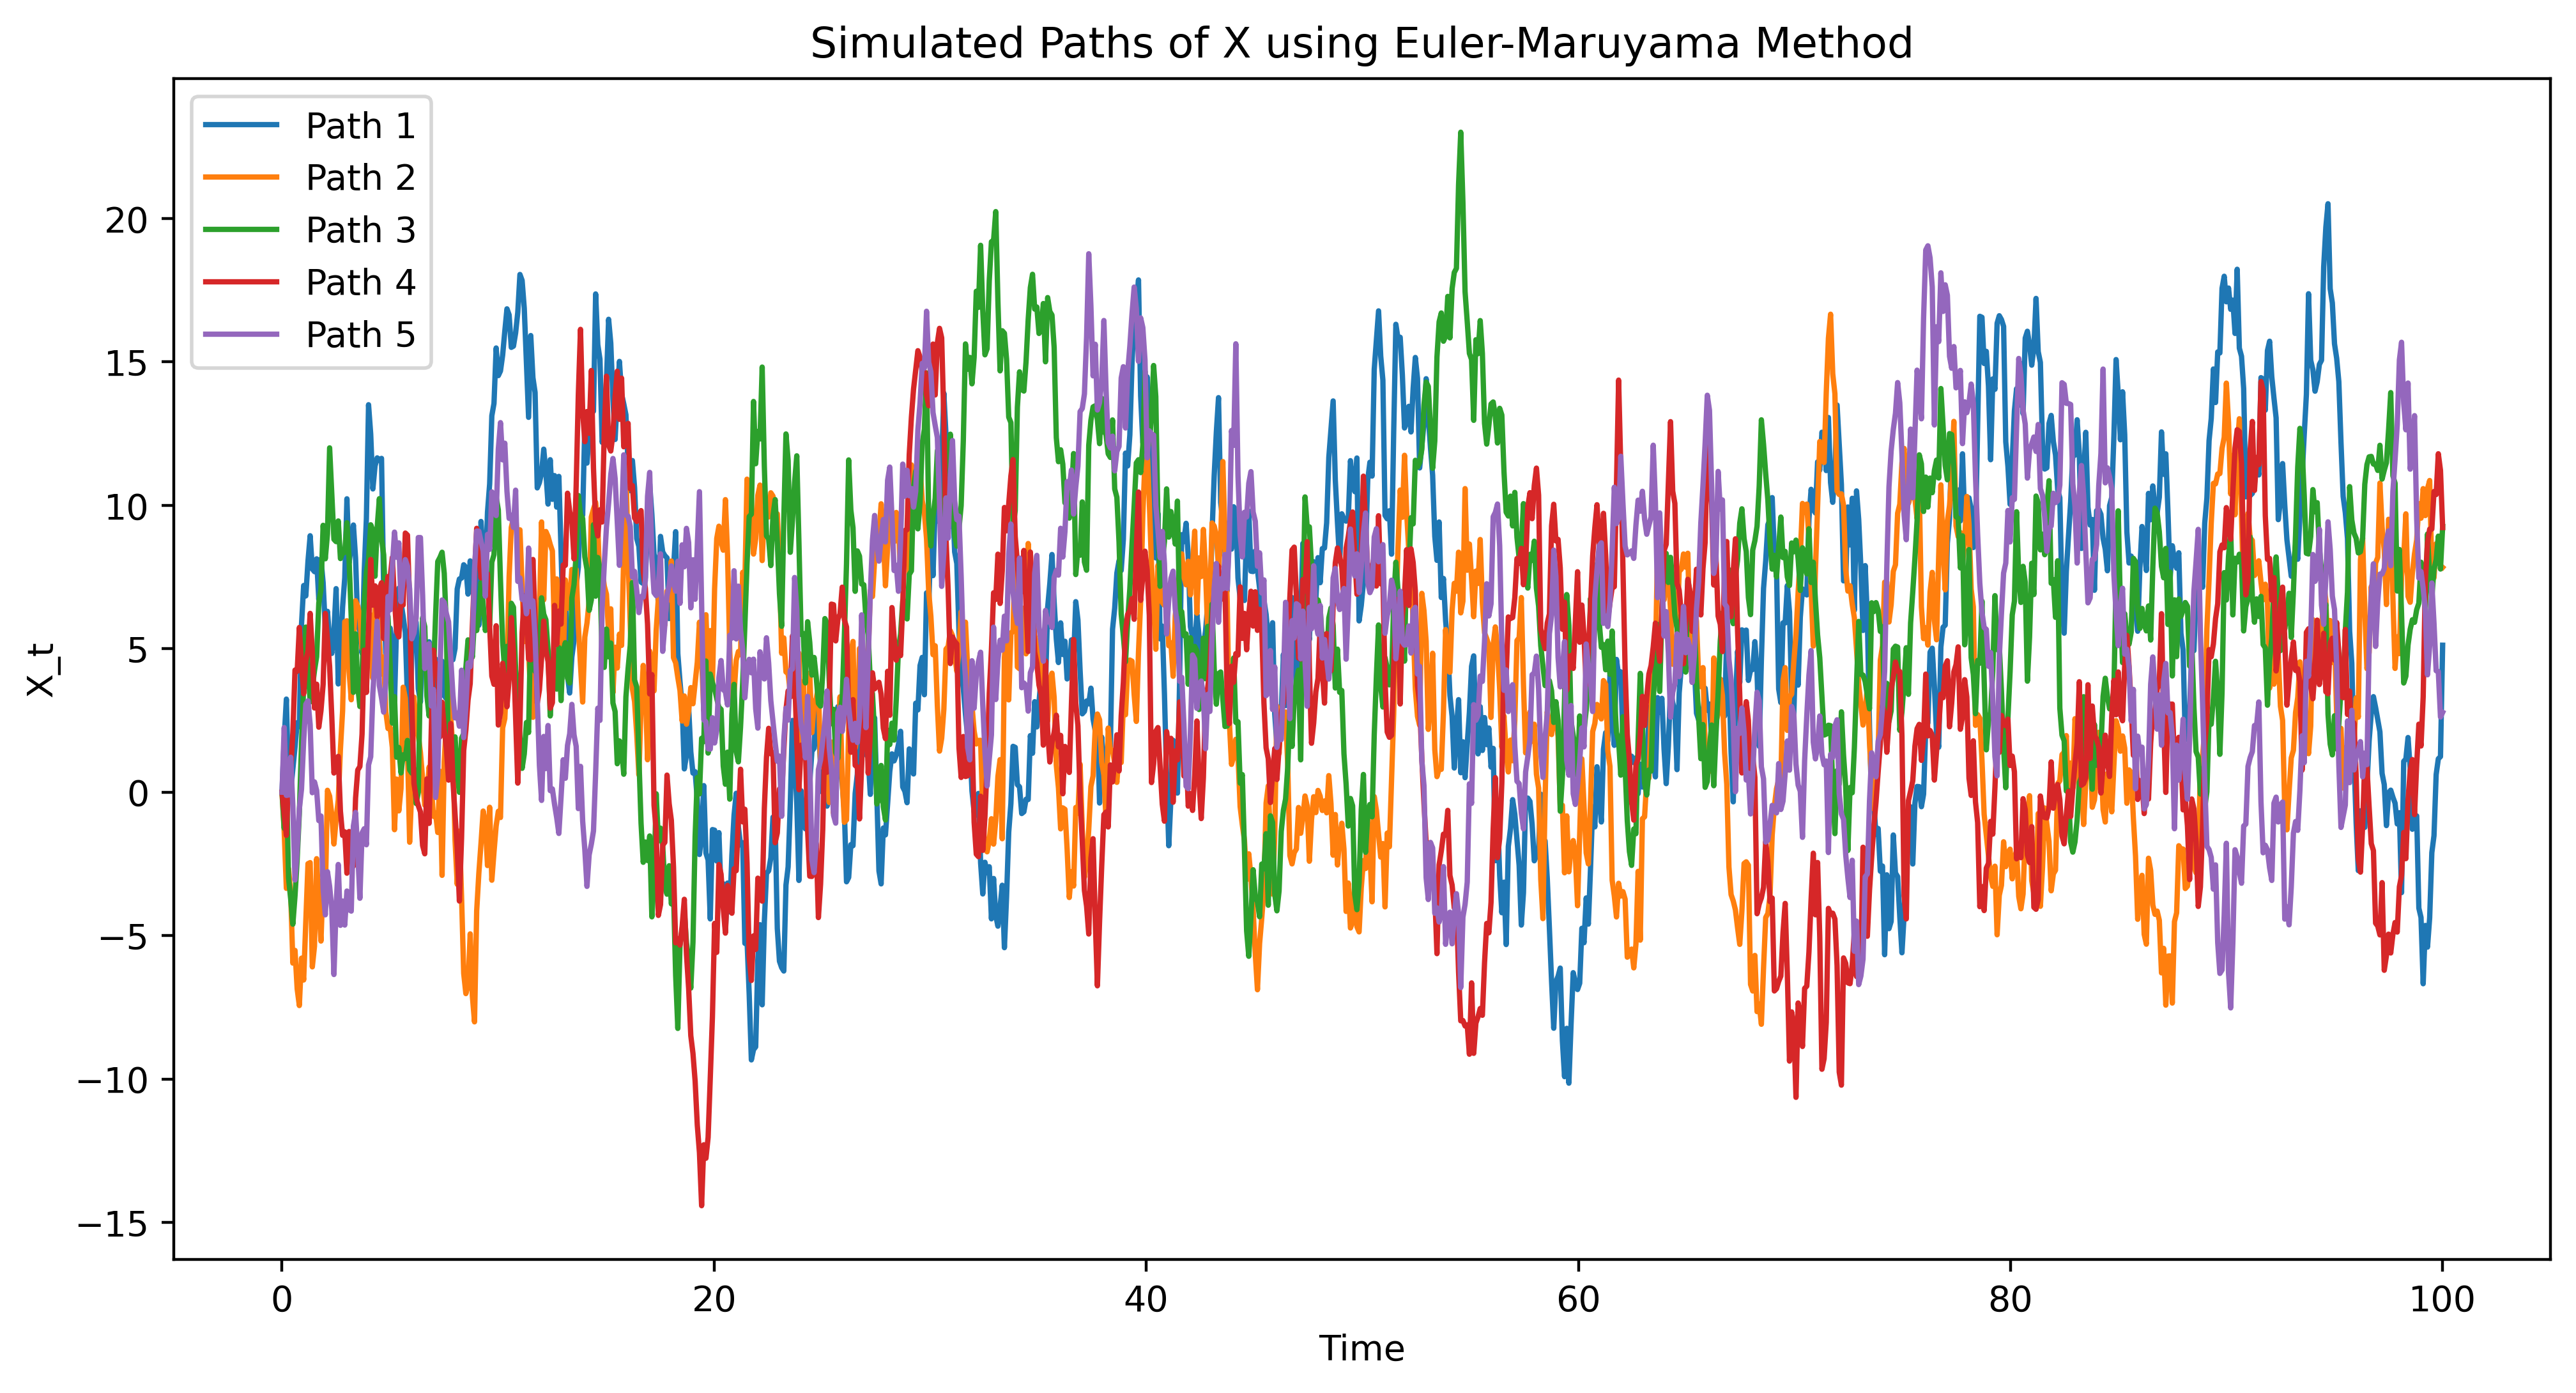
\includegraphics[width=.47\textwidth]{figures/EM4.png}}
    }
    \subfigure[模拟$X_t$轨道2阶变差]
    {
        {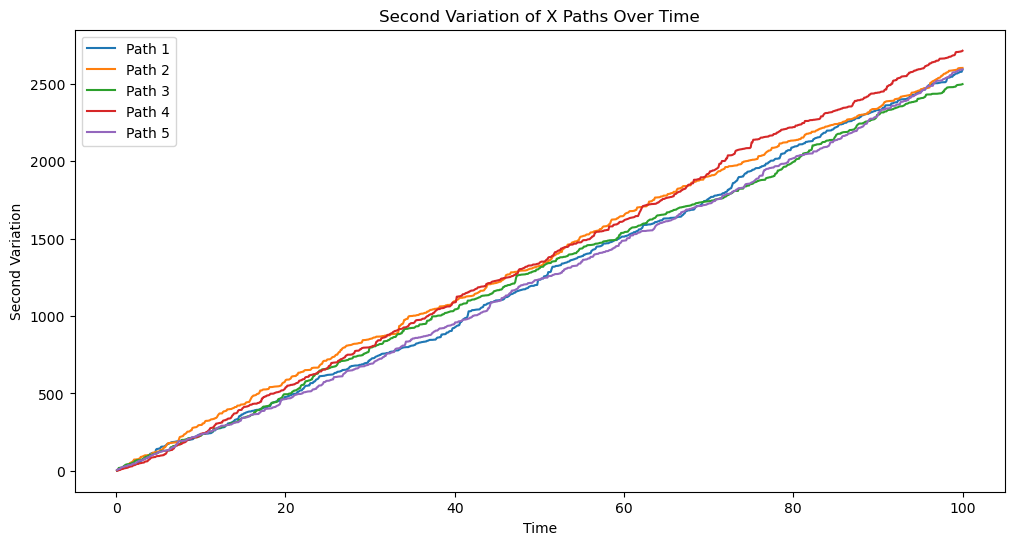
\includegraphics[width=.47\textwidth]{figures/EM42d.png}}
    }
\caption{$\alpha=0.5$, $v=5$,$sigma=5$, $x_0=0$}
\label{fig:EM4}
\end{figure}
\begin{figure}[t]
    \centering
    \subfigure[模拟$X_t$轨道]
    {
        {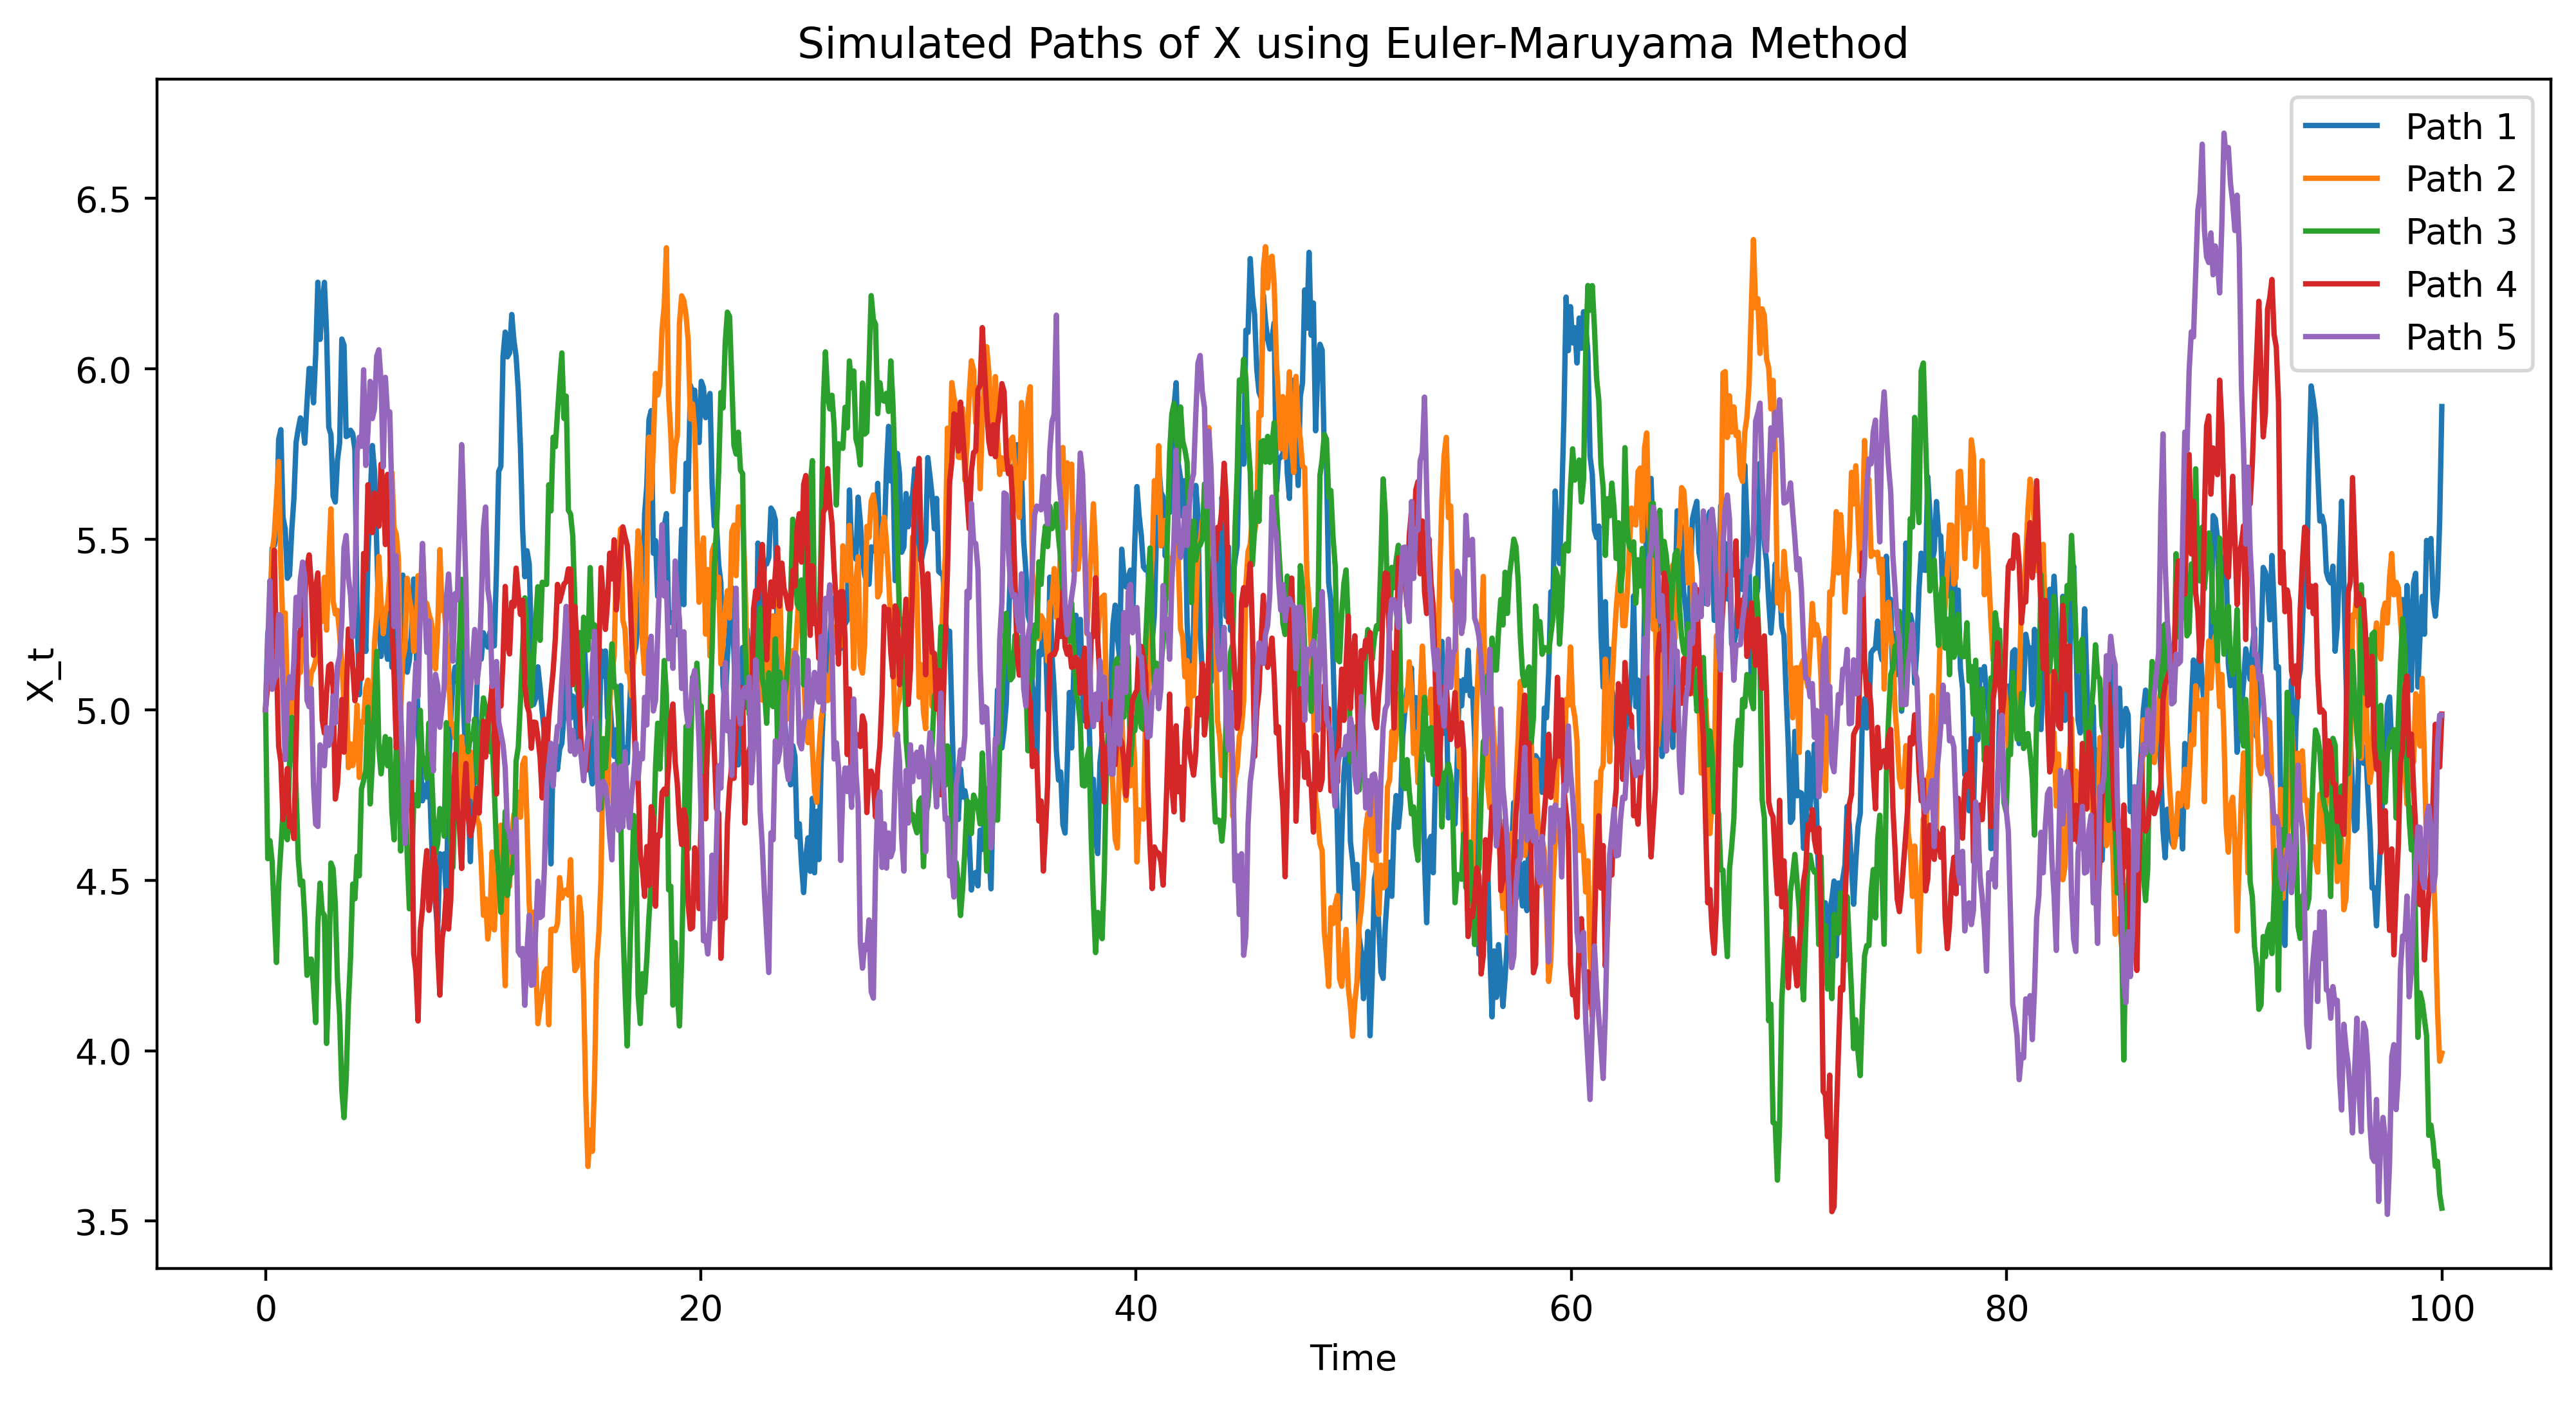
\includegraphics[width=.47\textwidth]{figures/EM5.png}}
    }
    \subfigure[模拟$X_t$轨道2阶变差]
    {
        {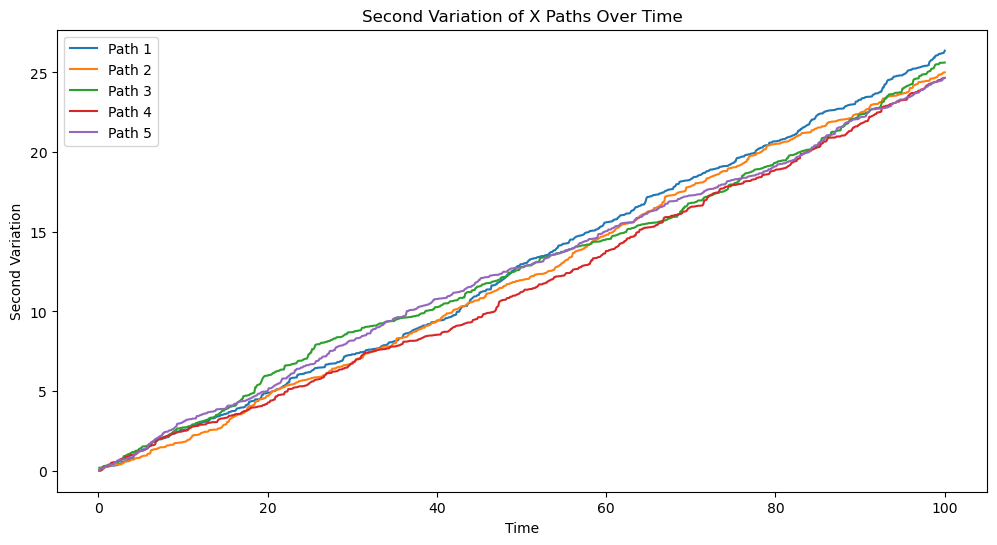
\includegraphics[width=.47\textwidth]{figures/EM52d.png}}
    }
\caption{$\alpha=0.5$, $v=5$,$sigma=0.5$, $x_0=5$}
\label{fig:EM5}
\end{figure}

\subsection{关于不同参数对于$X_t$轨道的影响}
我们选择5组不同参数
\begin{table}[h]
\centering
\begin{tabular}{|c|c|c|c|c|}
\hline
\textbf{组号} & $\boldsymbol{\alpha}$ & $\boldsymbol{v}$ & $\boldsymbol{\sigma}$ & $\boldsymbol{x_0}$ \\ 
\toprule
1             & 0.5                   & 5                & 0.5                   & 0                  \\ \hline
2             & 0.5                   & 0                & 0.5                   & 0                  \\ \hline
3             & 5                     & 5                & 0.5                   & 0                  \\ \hline
4             & 0.5                   & 5                & 5                     & 0                  \\ \hline
5             & 0.5                   & 5                & 0.5                   & 5                  \\ 
\bottomrule
\end{tabular}
\caption{不同参数组合对随机微分方程影响的比较}
\label{tab:parameter_sets}
\end{table}

当然,让我们讨论参数 \( \alpha, v, \sigma, x_0 \) 对于随机微分方程 \( dX_t = \alpha (v - X_t) dt + \sigma dB_t, \, X_0 = x_0 \) 的解 \( X_t \) 的轨道所产生的影响:
\begin{enumerate}
    \item 参数 \( \alpha \)(衰减系数)
    \par \( \alpha \) 控制着系统对偏离其均值 \( v \) 的响应速度。较大的 \( \alpha \) 值意味着 \( X_t \) 会更快地向其均值 \( v \) 回归。如果 \( \alpha \) 很小,\( X_t \) 的变化将更加缓慢和温和,轨迹会更平滑。
    \item 参数 \( v \)(均值
    \par \( v \) 是 \( X_t \) 的长期均值或均值回归目标。随着时间的推移,\( X_t \) 的轨迹会趋向于接近这个值。改变 \( v \) 的值会改变轨迹的中心或平衡位置。

    \item 参数 \( \sigma \)(波动性)
    \par \( \sigma \) 控制着布朗运动部分对 \( X_t \) 轨迹的影响,它代表了轨迹的波动性或不确定性。较高的 \( \sigma \) 值导致更大的随机波动,使轨迹变得更不稳定和不可预测。

    \item 初始值 \( x_0 \)(初始位置)
    \par \( x_0 \) 是 \( X_t \) 起始时刻的值。它决定了轨迹的起始点。虽然初始值对轨迹的长期行为影响较小(特别是在 \( \alpha \) 较大时),但它会影响轨迹的短期动态。


\end{enumerate}
总体而言,这些参数共同决定了 \( X_t \) 的行为,包括它如何随时间演变、它的波动程度,以及它如何响应随机扰动。通过改变这些参数,我们可以观察到不同的随机过程行为,从而更好地理解和解释这些过程的动态特性。
\par
当我们讨论不同的 \( \alpha, v, \sigma, x_0 \) 常数对于随机微分方程 \( dX_t = \alpha (v - X_t) dt + \sigma dB_t, \, X_0 = x_0 \) 的解 \( X_t \) 的二阶变差轨道的影响的时候,我们可以考虑到:

\begin{enumerate}
    \item 参数 \( \alpha \)(衰减系数)
    \par \( \alpha \) 决定了 \( X_t \) 对其均值 \( v \) 的回归速度。较大的 \( \alpha \) 会导致 \( X_t \) 更快地向 \( v \) 调整,从而可能减少因随机波动导致的偏离。较小的 \( \alpha \) 值允许更多的随机波动影响轨迹,可能增加二阶变差,因为路径在达到稳定状态之前会有更多的波动。
    \item 参数 \( v \)(均值
    \par \( v \) 是 \( X_t \) 的长期均值或均值回归目标。更改 \( v \) 的值不会直接影响二阶变差,因为它更多地影响轨迹的中心位置而不是其波动性。

    \item 参数 \( \sigma \)(波动性)
    \par \( \sigma \) 直接控制了布朗运动部分的影响,即轨迹的波动性。较高的 \( \sigma \) 值会导致更大的随机波动,从而增加二阶变差,因为路径变得更加不稳定和不可预测。

    \item 初始值 \( x_0 \)(初始位置)
    \par \( x_0 \) 是初始时刻 \( X_t \) 的值。虽然初始值对轨迹的长期行为影响较小,但它可能会影响轨迹在短期内的波动,特别是如果 \( x_0 \) 与均值 \( v \) 相差很大时。

\end{enumerate}

总结来说,\( \alpha \) 和 \( \sigma \) 对 \( X_t \) 的二阶变差有直接影响,其中 \( \alpha \) 影响轨迹如何响应均值回归,而 \( \sigma \) 控制了轨迹的整体波动性。相比之下,\( v \) 和 \( x_0 \) 对二阶变差的影响较小,主要影响轨迹的位置而非波动性。

\section{分析两个相互作用的SDE}
问题3对应的随机微分方程系统描述了两个互相关联的过程 \( X_t \) 和 \( S_t \),每个过程都由不同的动态和随机因素驱动。这个系统可以用来模拟各种现实世界中的现象,比如金融资产的价格和其衍生变量的行为。下面是对这些方程的分析:
\begin{enumerate}
    \item \( dX_t = \alpha(v - X_t)dt + \sigma dB_t \)
    \begin{itemize}
        \item \( X_t \) 表示的变量趋向于长期均值 \( v \)
        \item \( \alpha \) 控制着 \( X_t \) 回归到 \( v \) 的速度
        \item \( \sigma dB_t \) 项引入了随机性,其中 \( B_t \) 是一个标准布朗运动。
    \end{itemize}
    \item \( dS_t = \theta(X_t - S_t)dt + \tilde{\sigma}_1 dB_t + \tilde{\sigma}_2 dW_t \)
    \begin{itemize}
        \item \( S_t \) 的动态类似于 \( X_t \),但它还受到 \( X_t \) 当前值的影响,这表示 \( S_t \) 可能试图跟踪或响应 \( X_t \) 的变化
        \item \( \theta \) 控制了 \( S_t \) 对 \( X_t \) 的响应速度
        \item \( \tilde{\sigma}_1 dB_t + \tilde{\sigma}_2 dW_t \) 表明 \( S_t \) 受到两个独立布朗运动的影响,增加了系统的复杂性和随机性
    \end{itemize}
\end{enumerate}

\subsection{电脑模拟生成}
如果想要进行,使用Euler-Maruyama方法进行数值模拟时,我们可以写出以下近似公式:

1. 对于 \( X_t \):

   \[ X_{t+\Delta t} = X_t + \alpha(v - X_t)\Delta t + \sigma \sqrt{\Delta t} \, \epsilon_{t,1} \]

   其中,\( \epsilon_{t,1} \) 是从标准正态分布中抽取的随机样本,用于模拟 \( dB_t \)。

2. 对于 \( S_t \):

   \[ S_{t+\Delta t} = S_t + \theta(X_t - S_t)\Delta t + \tilde{\sigma}_1 \sqrt{\Delta t} \, \epsilon_{t,1} + \tilde{\sigma}_2 \sqrt{\Delta t} \, \epsilon_{t,2} \]

   其中,\( \epsilon_{t,2} \) 是另一个独立的从标准正态分布中抽取的随机样本,用于模拟 \( dW_t \)。

这些公式提供了在每个时间步长 \( \Delta t \) 上对两个过程 \( X_t \) 和 \( S_t \) 进行迭代的方法。通过从初始条件 \( X_0 = x_0 \) 和 \( S_0 = s_0 \) 开始,我们可以使用这些公式逐步构建整个轨迹。这种方法允许我们在离散时间点上近似连续时间随机过程的行为,是研究这类系统的一种有效工具。
\begin{figure}[p]
    \centering
    \subfigure[模拟$X_t$和$S_t$轨道]
    {
        {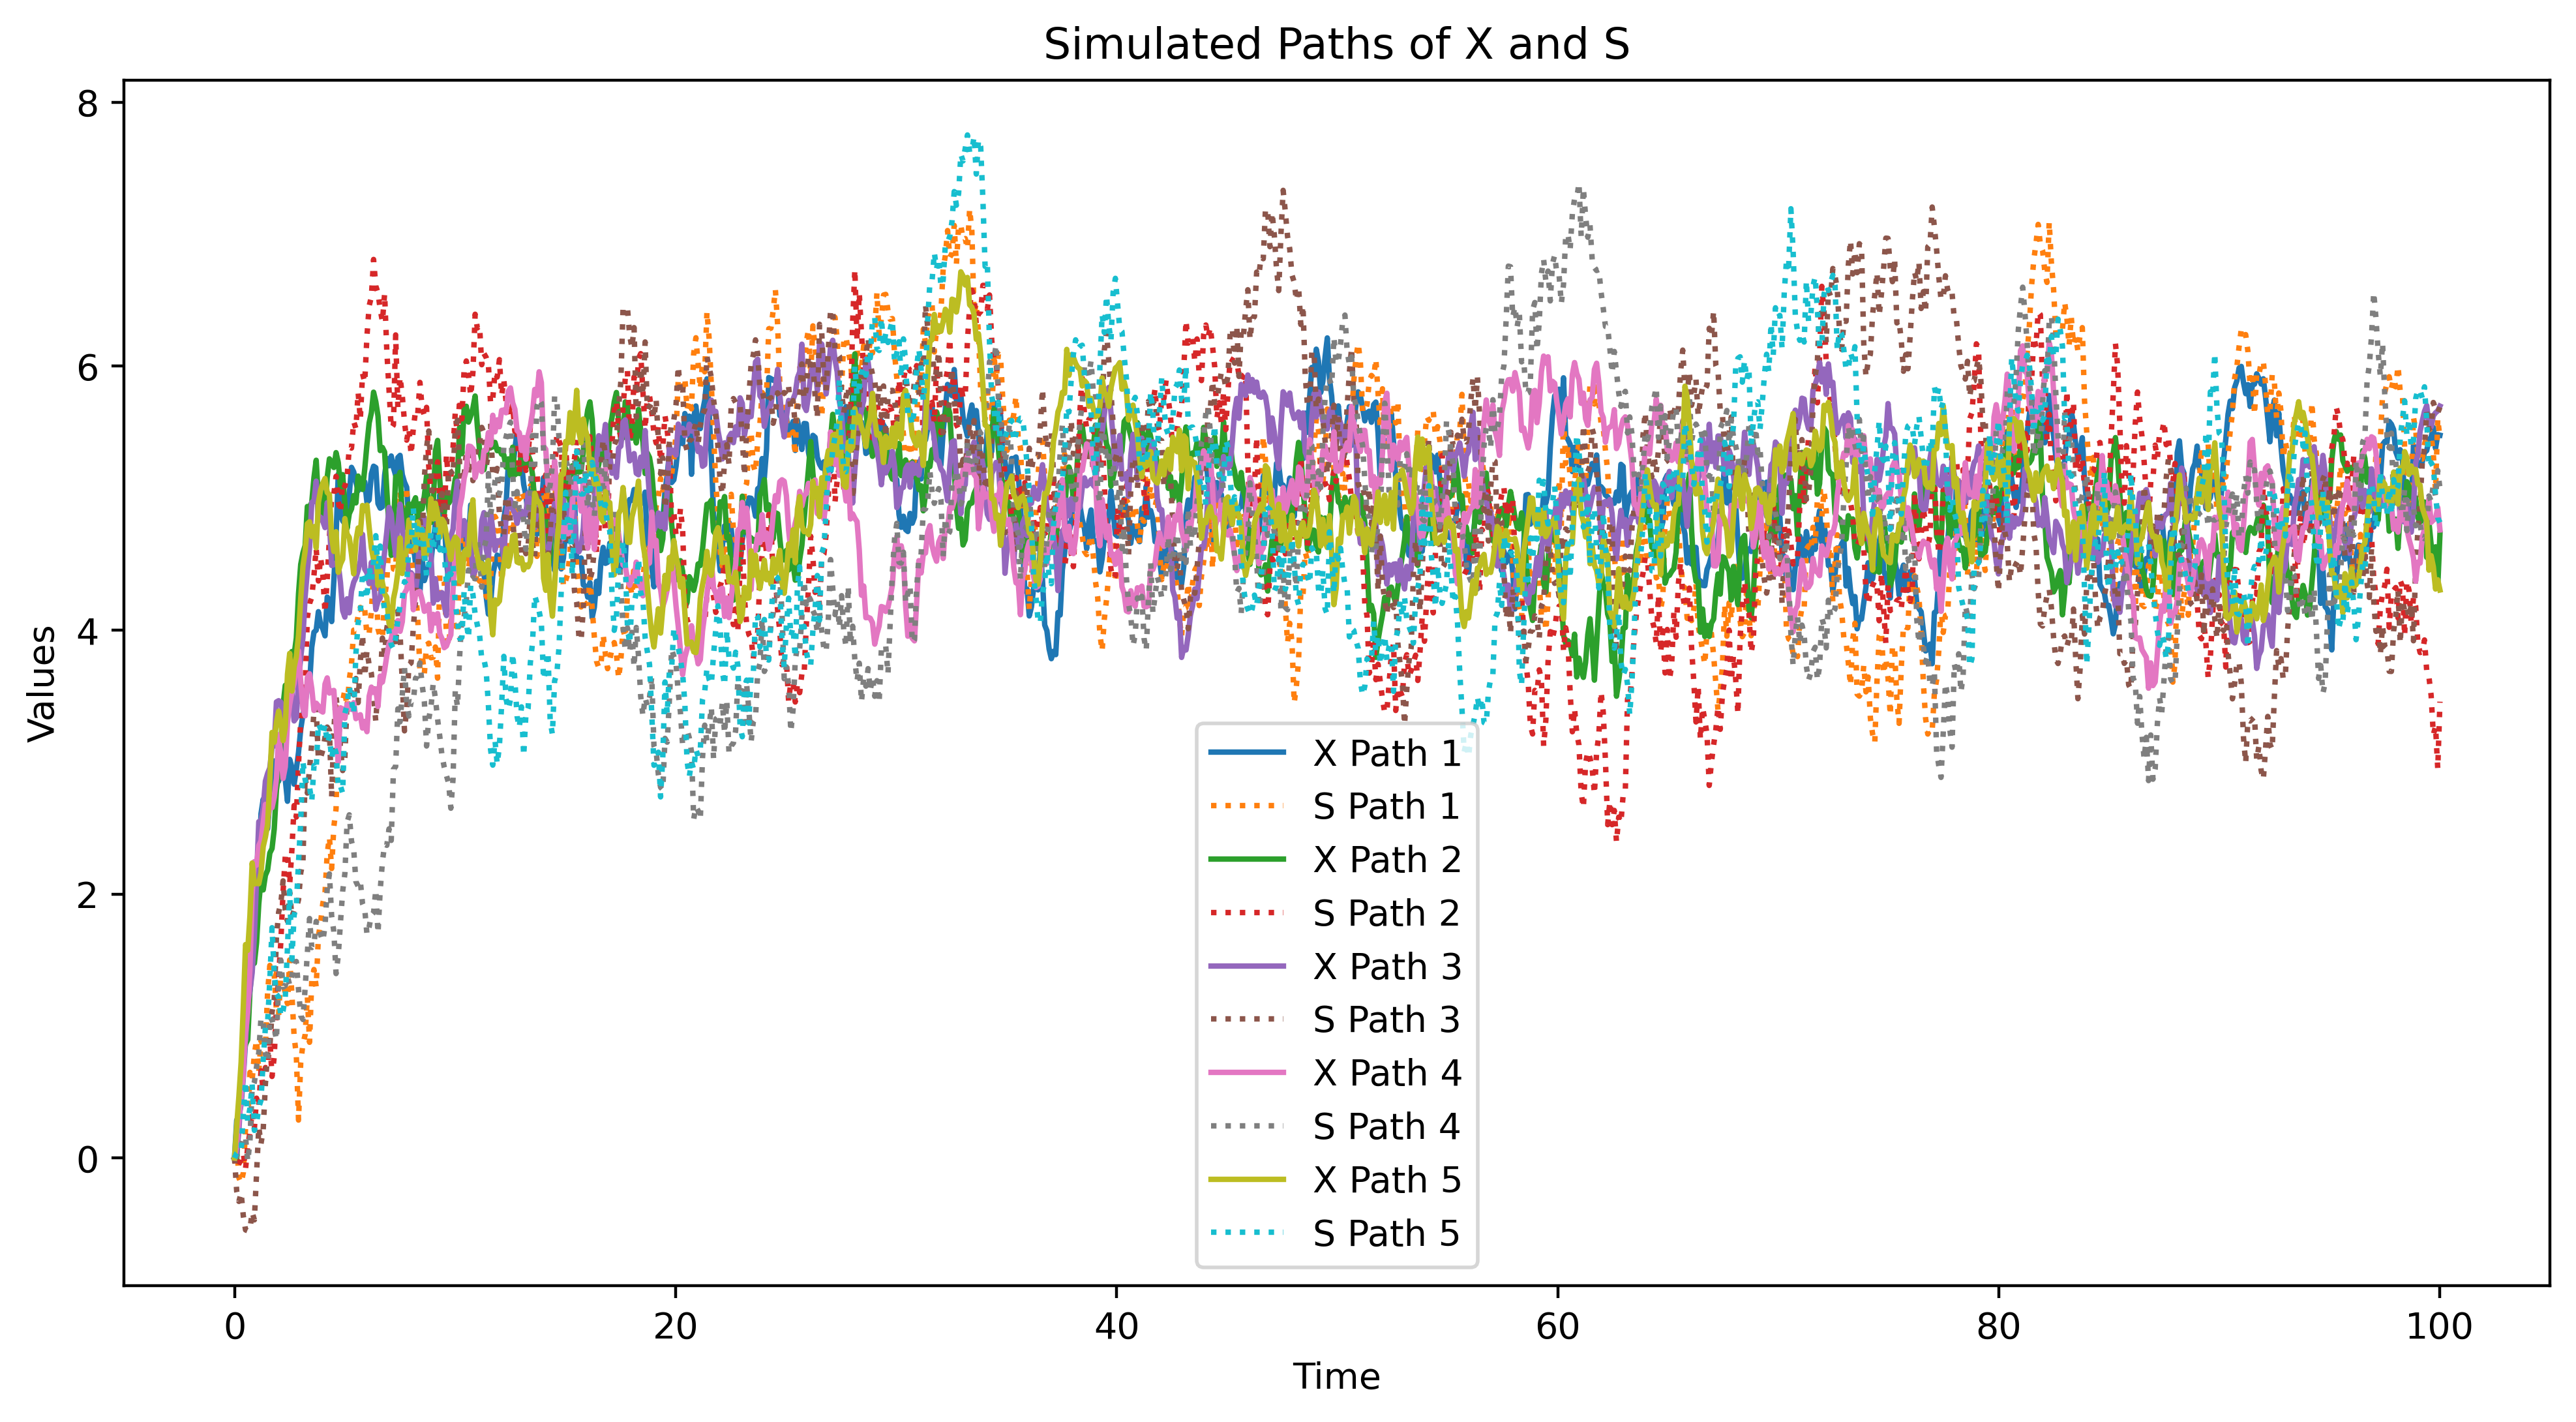
\includegraphics[width=.47\textwidth]{figures/XS1.png}}
    }
    \subfigure[模拟$X_t$和$S_t$轨道2阶变差]
    {
        {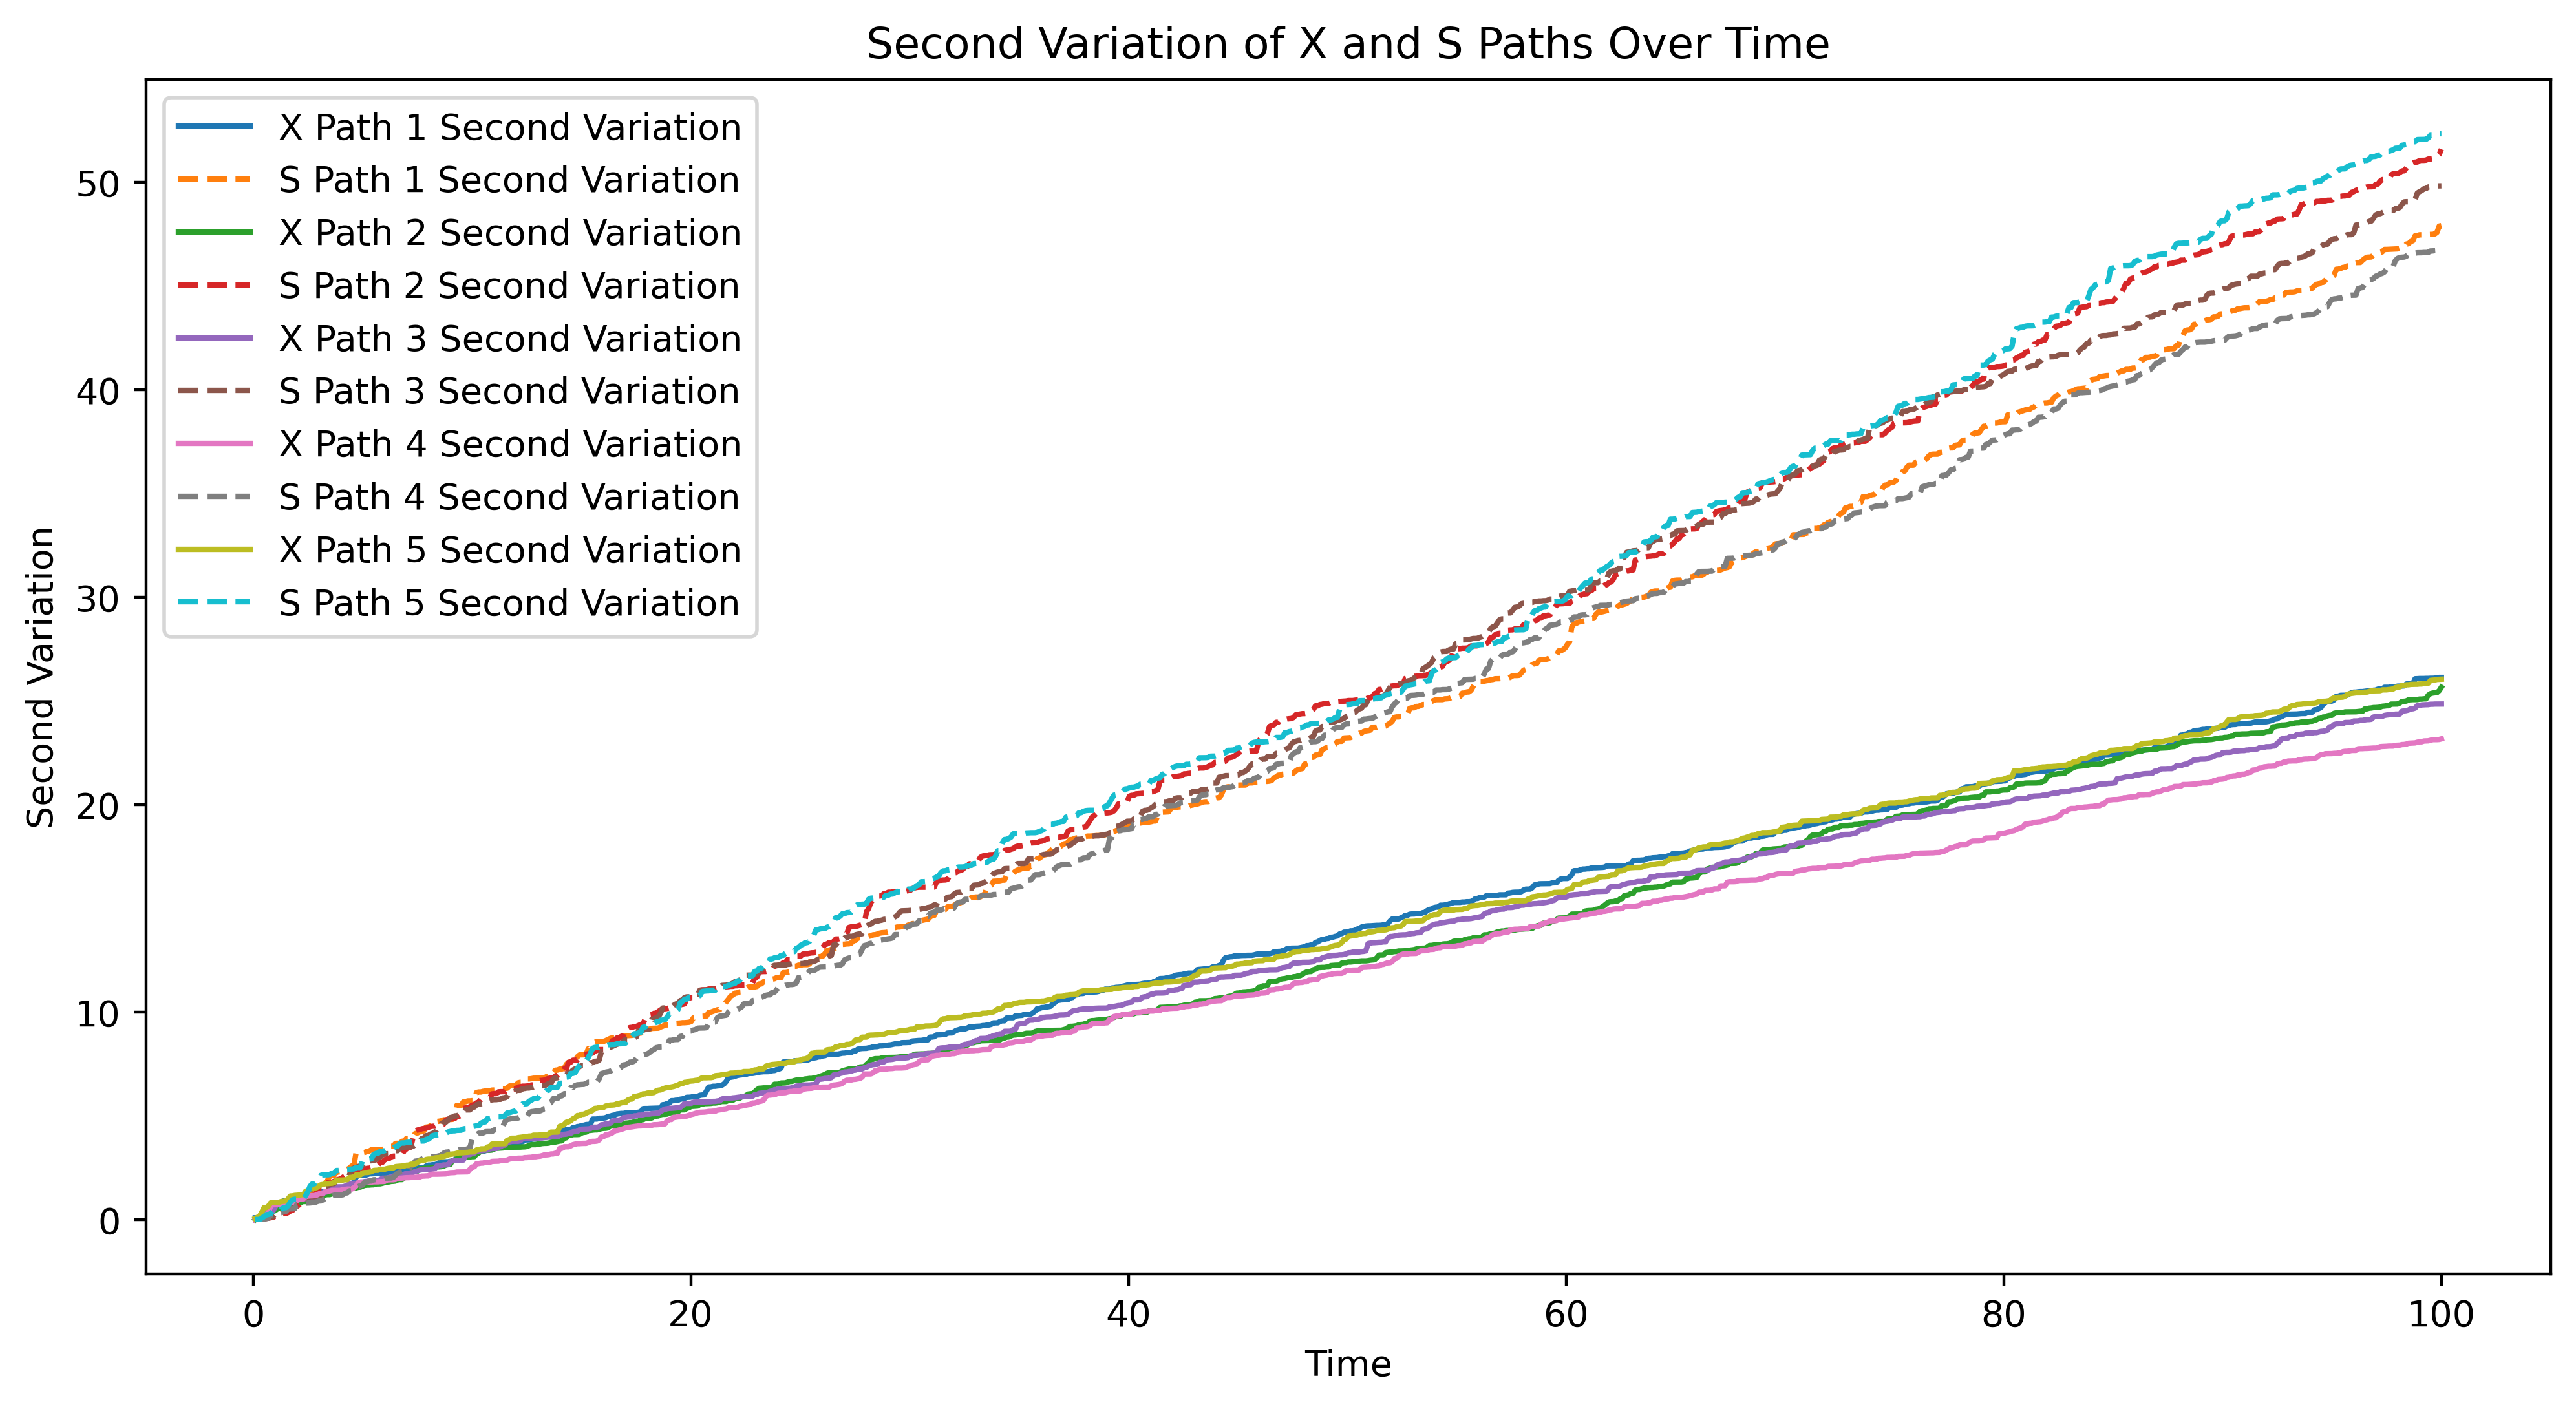
\includegraphics[width=.47\textwidth]{figures/XS1_2d.png}}
    }
    \centering
    \subfigure[模拟$X_t$和$S_t$轨道]
    {
        {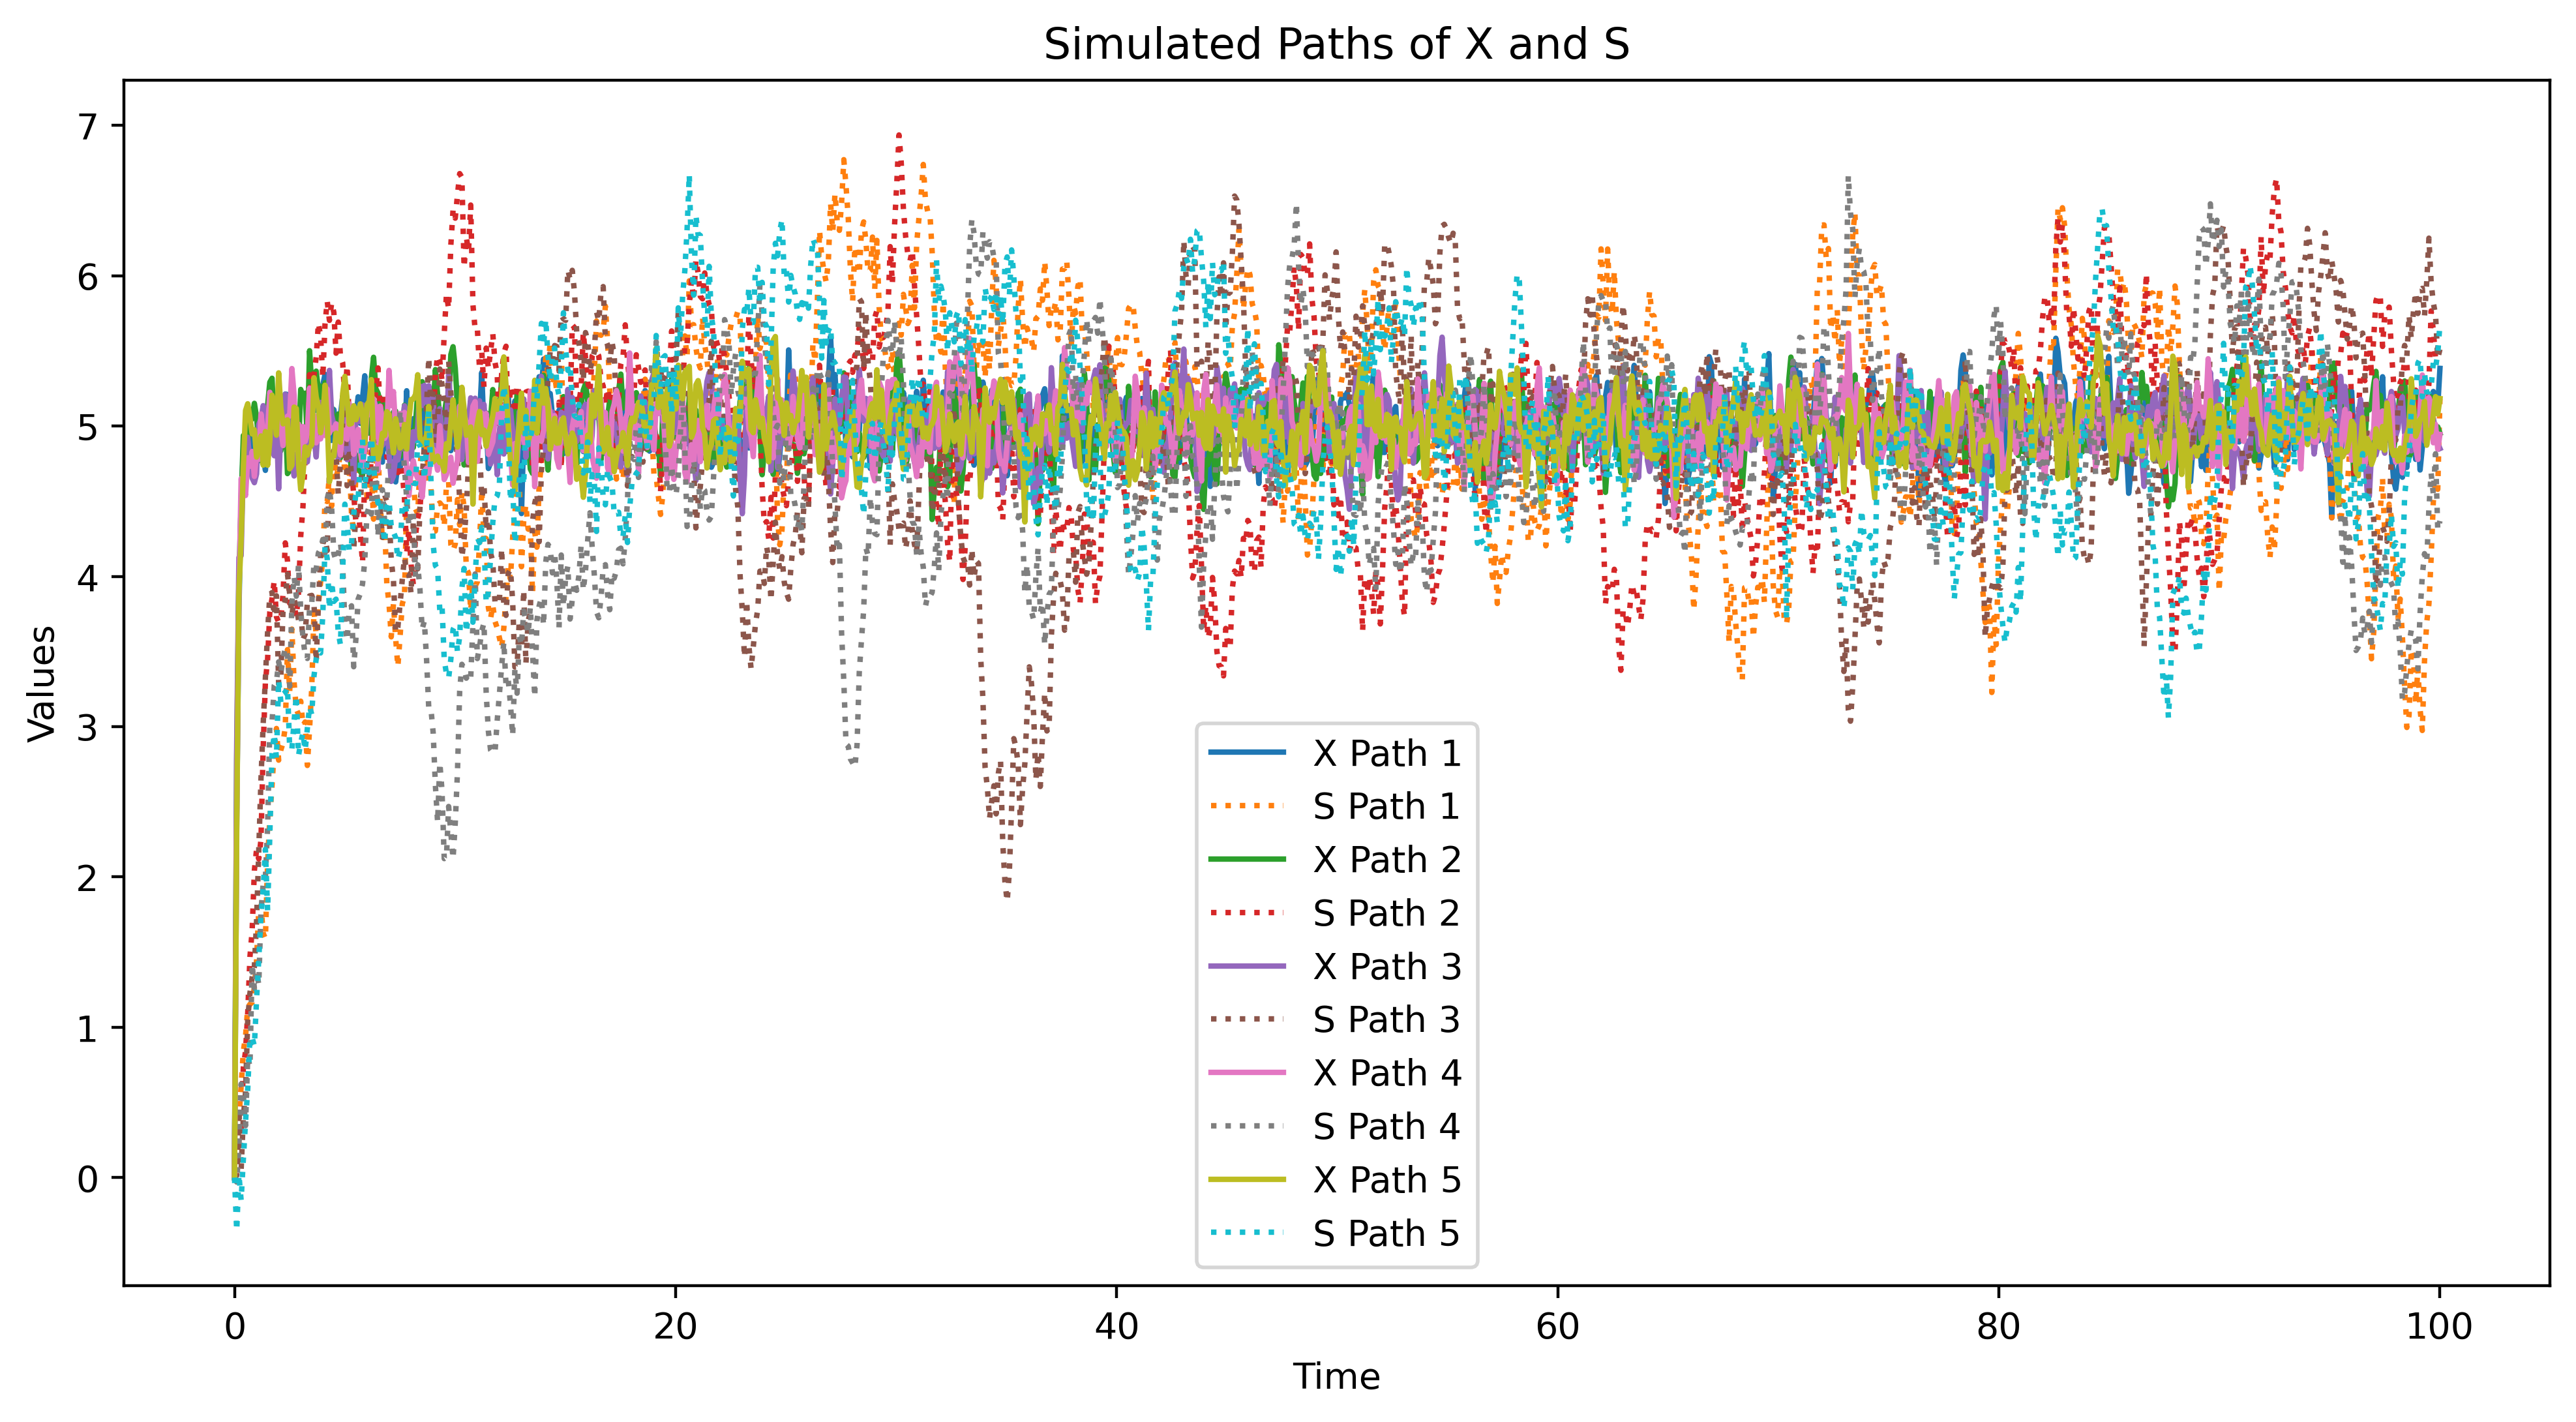
\includegraphics[width=.47\textwidth]{figures/XS2.png}}
    }
    \subfigure[模拟$X_t$和$S_t$轨道2阶变差]
    {
        {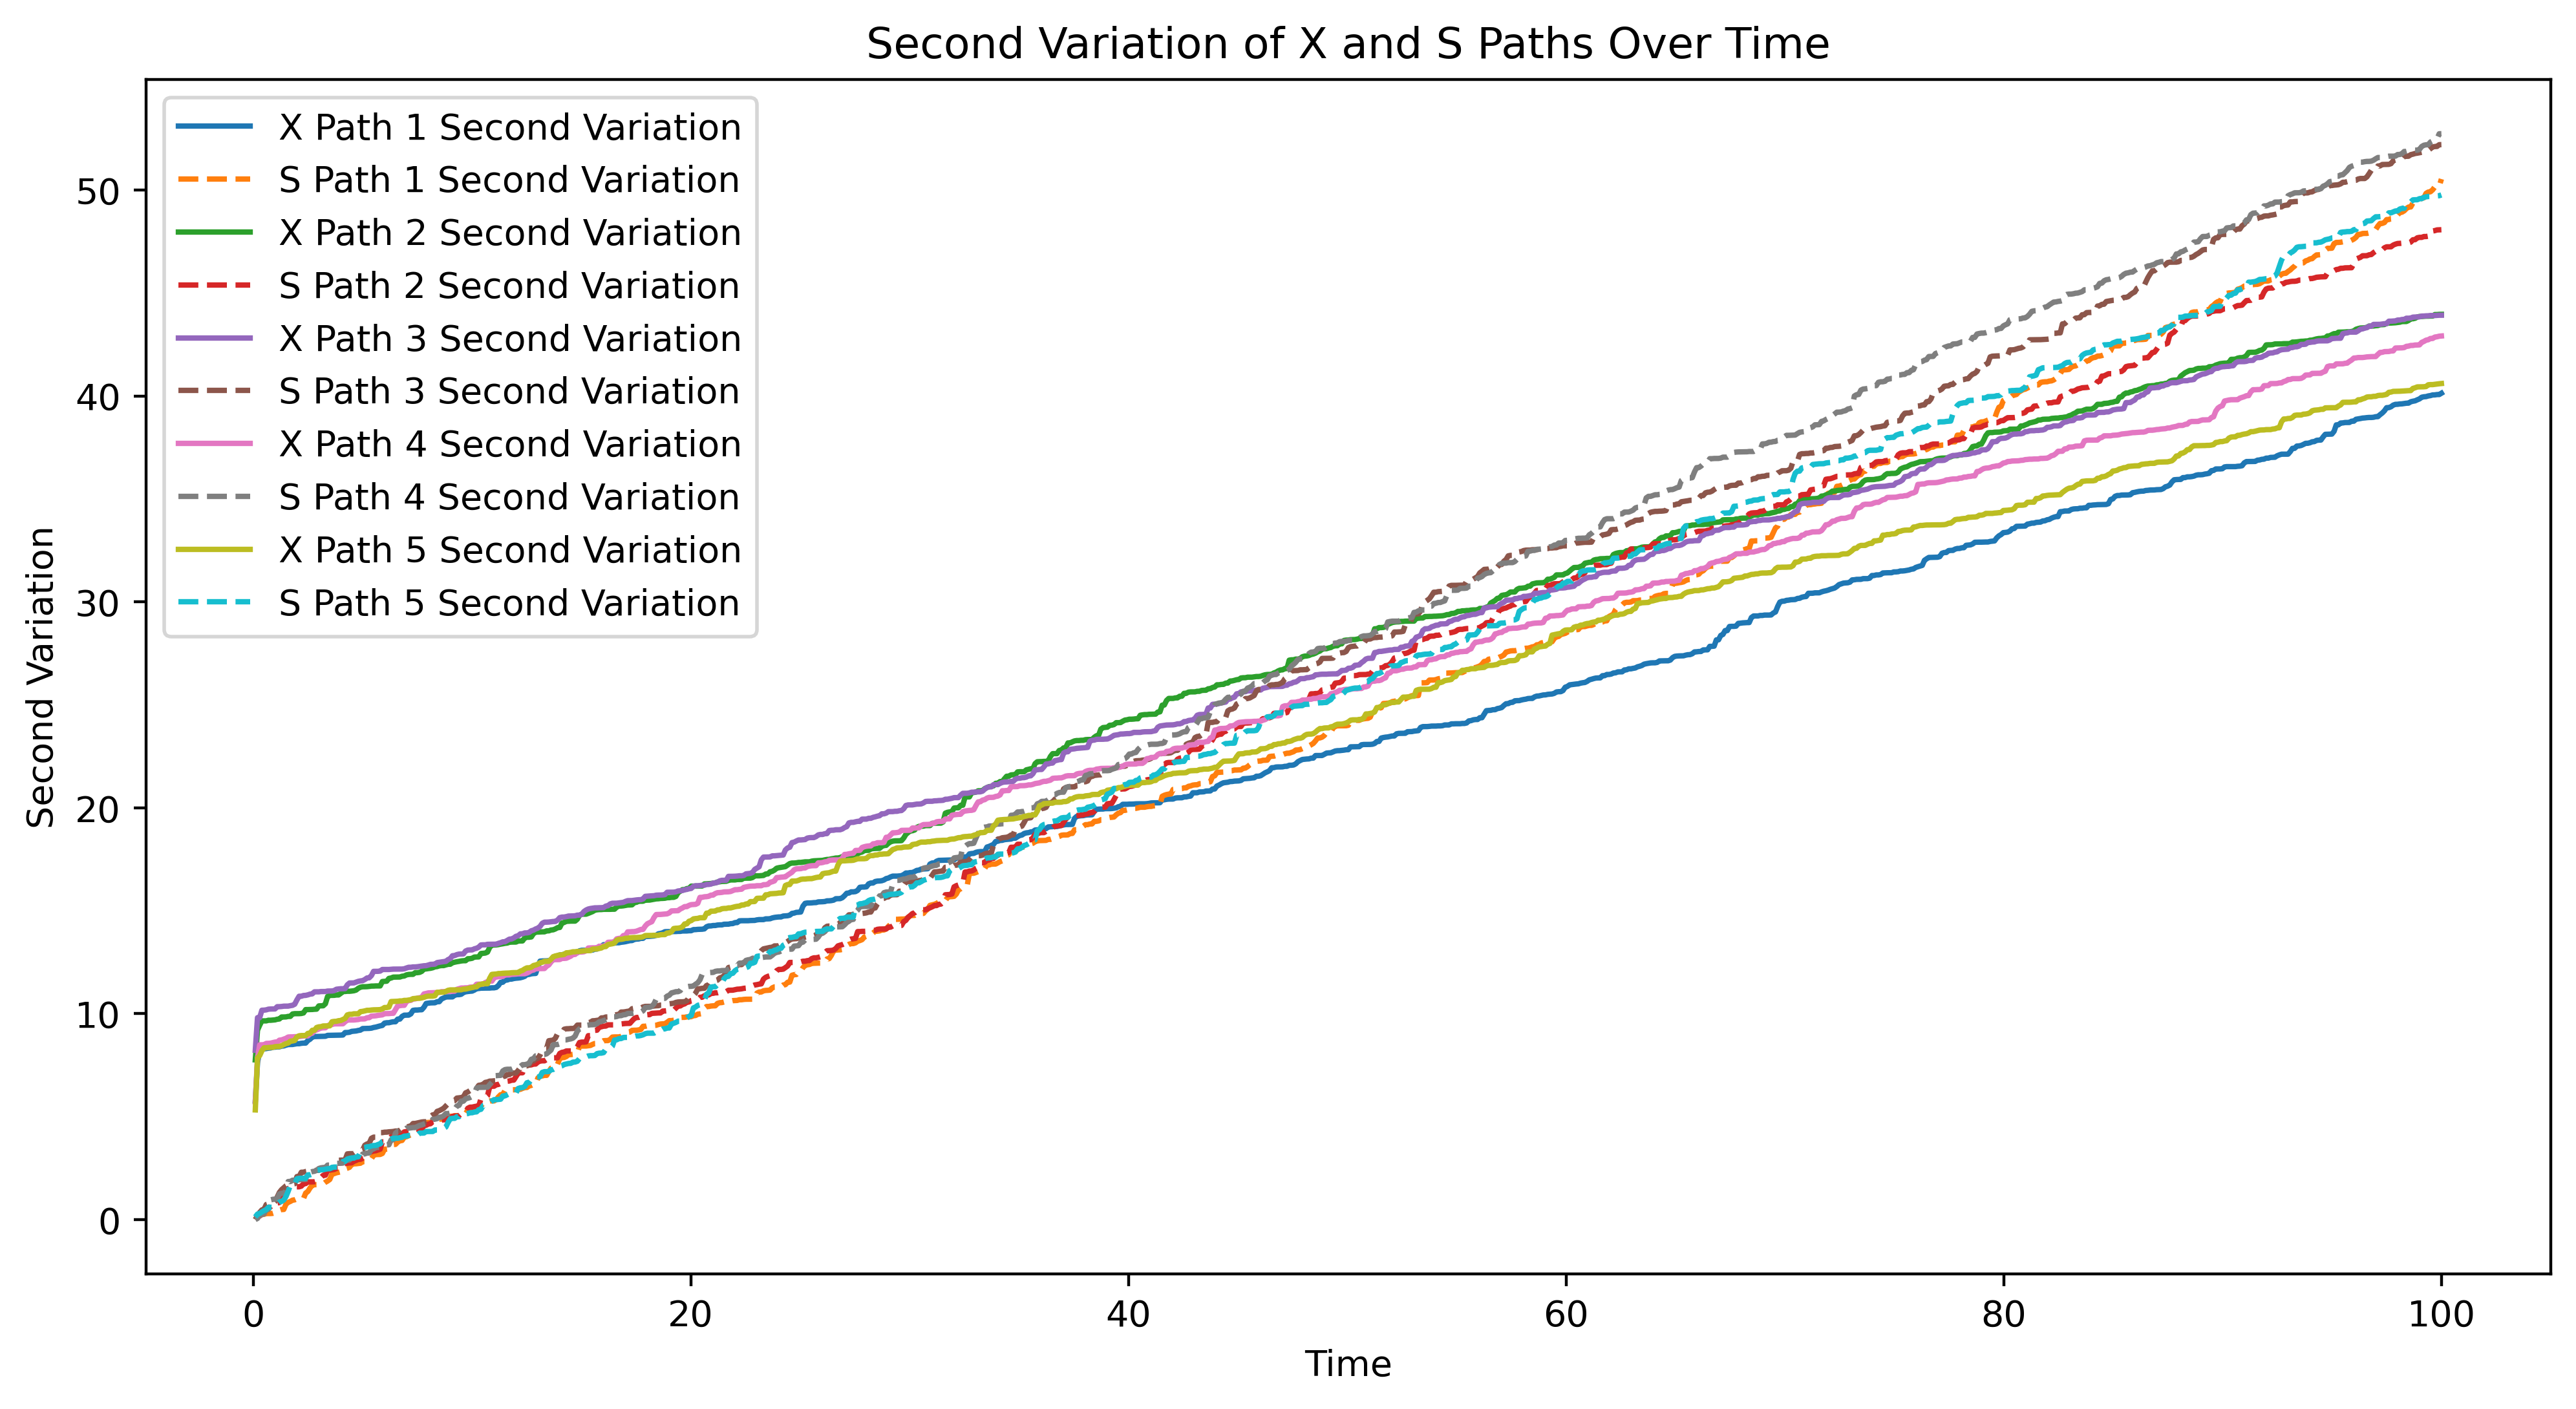
\includegraphics[width=.47\textwidth]{figures/XS2_2d.png}}
    }
    \centering
    \subfigure[模拟$X_t$和$S_t$轨道]
    {
        {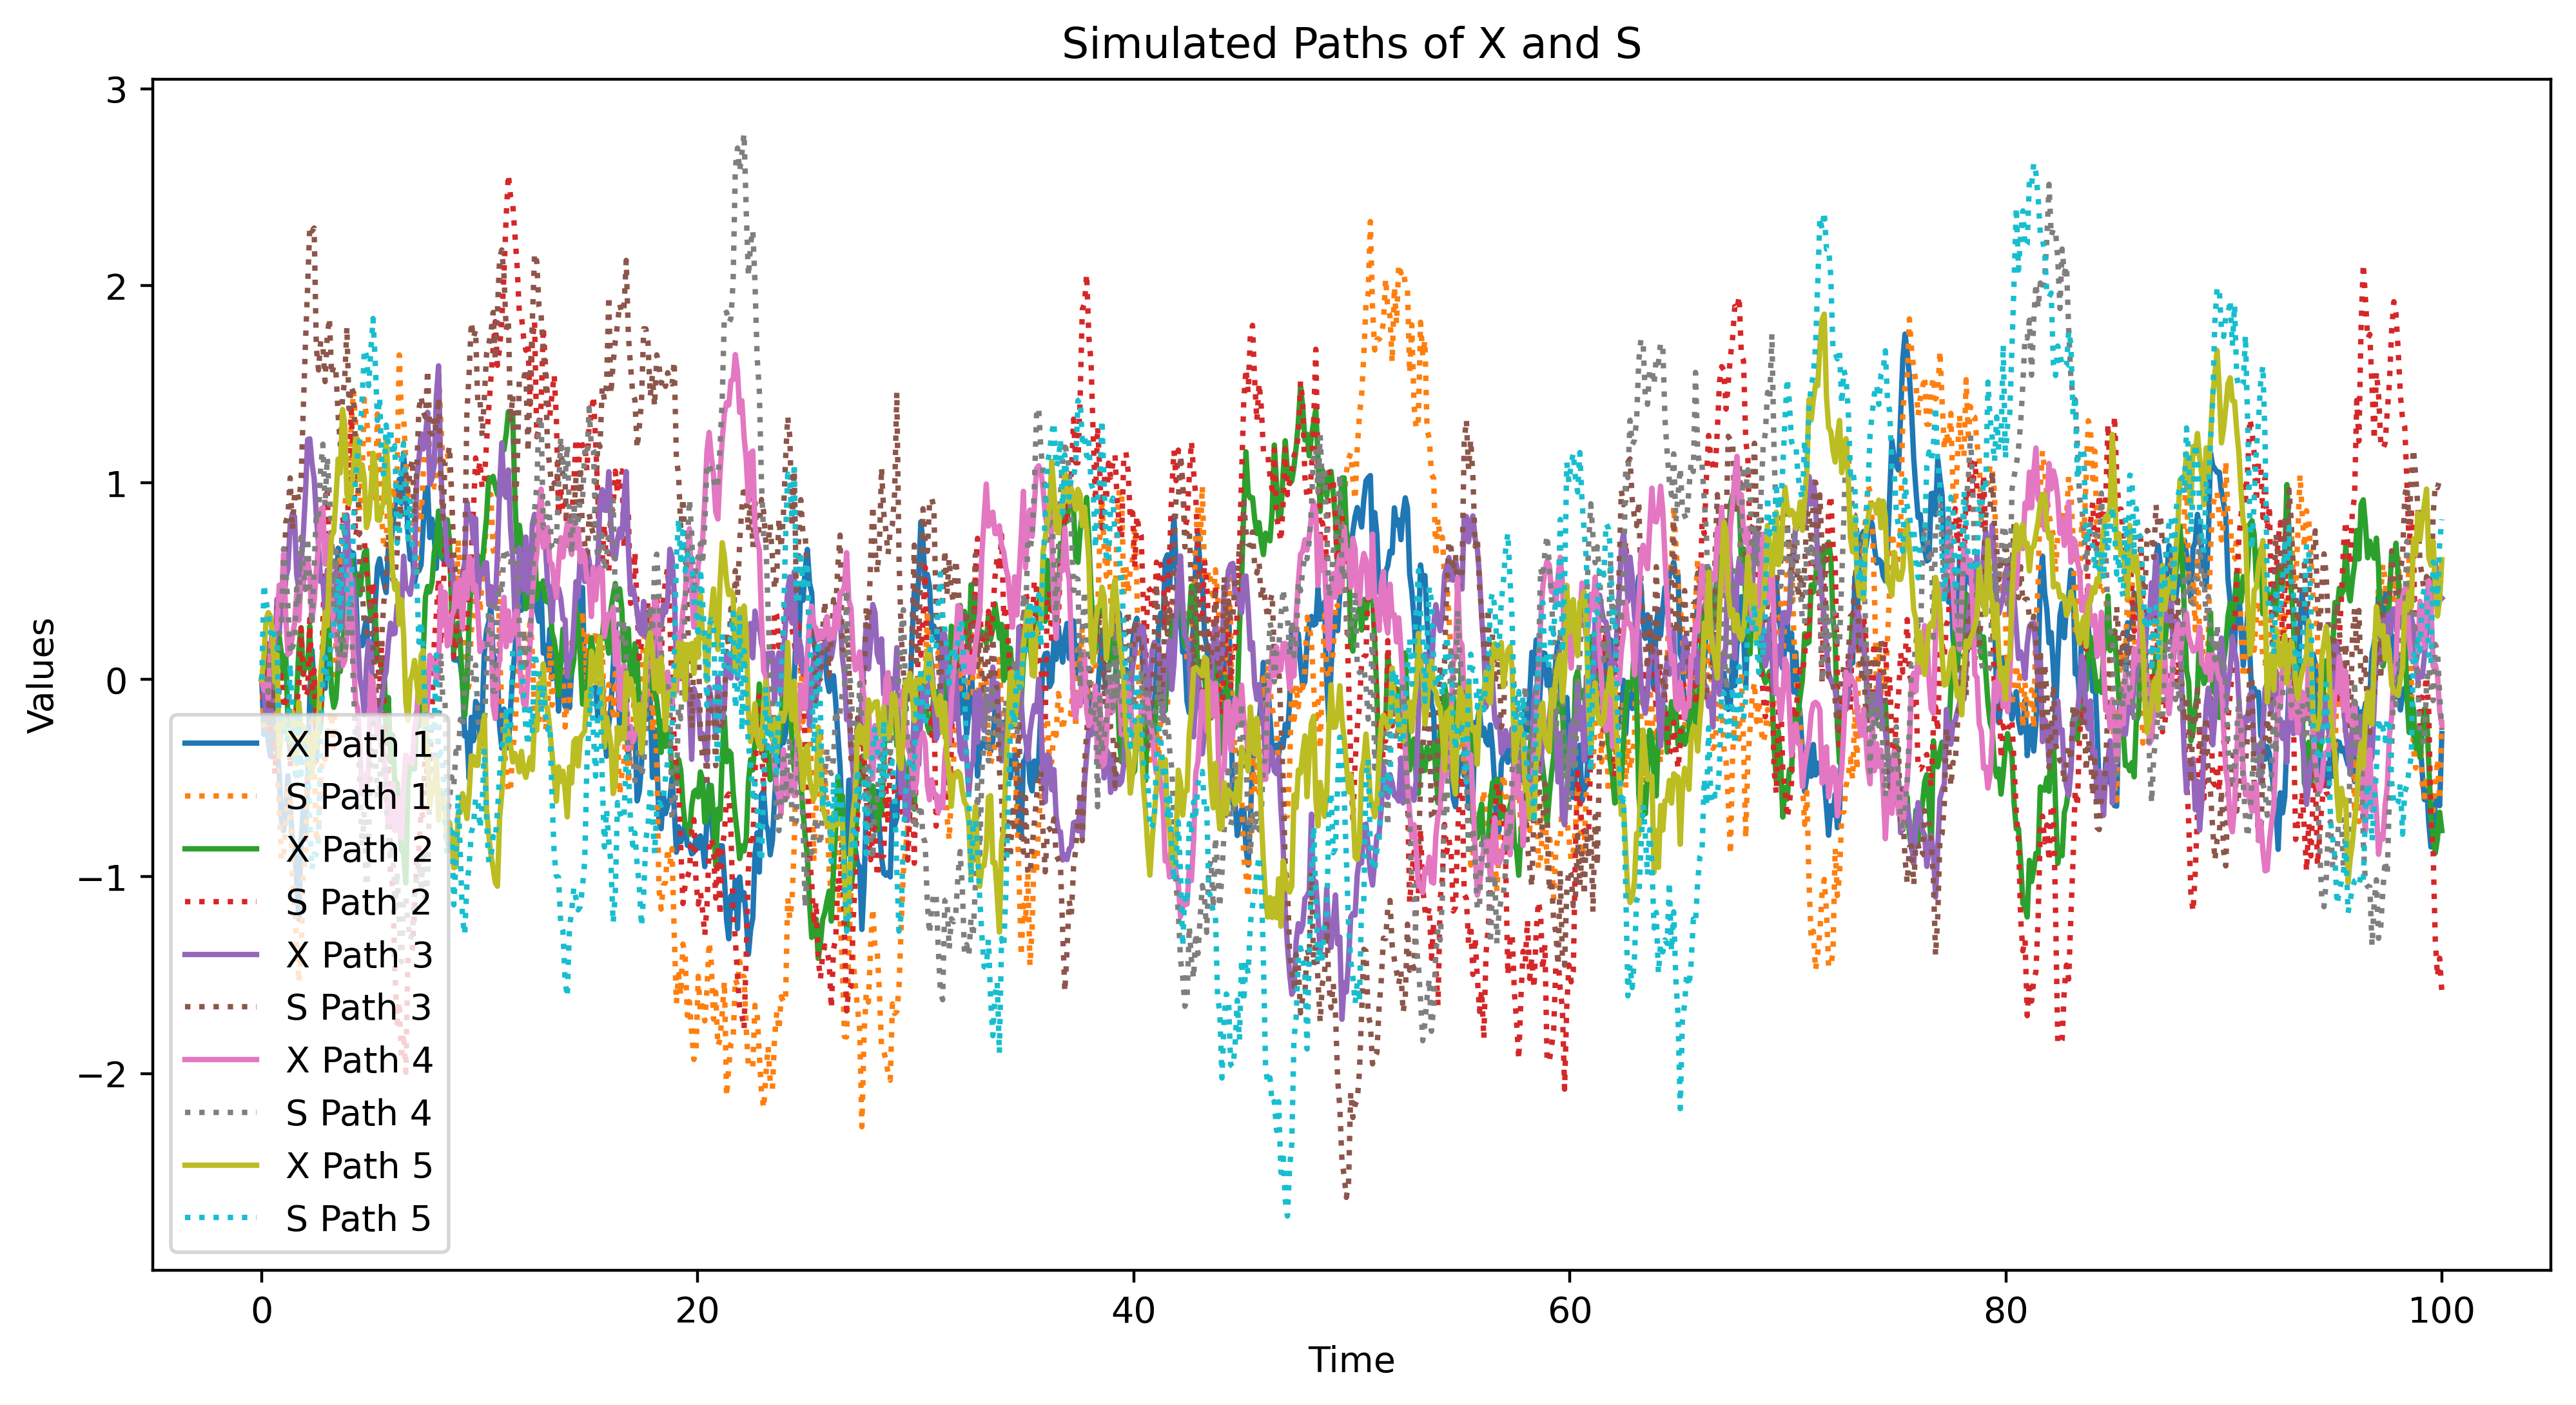
\includegraphics[width=.47\textwidth]{figures/XS3.png}}
    }
    \subfigure[模拟$X_t$和$S_t$轨道2阶变差]
    {
        {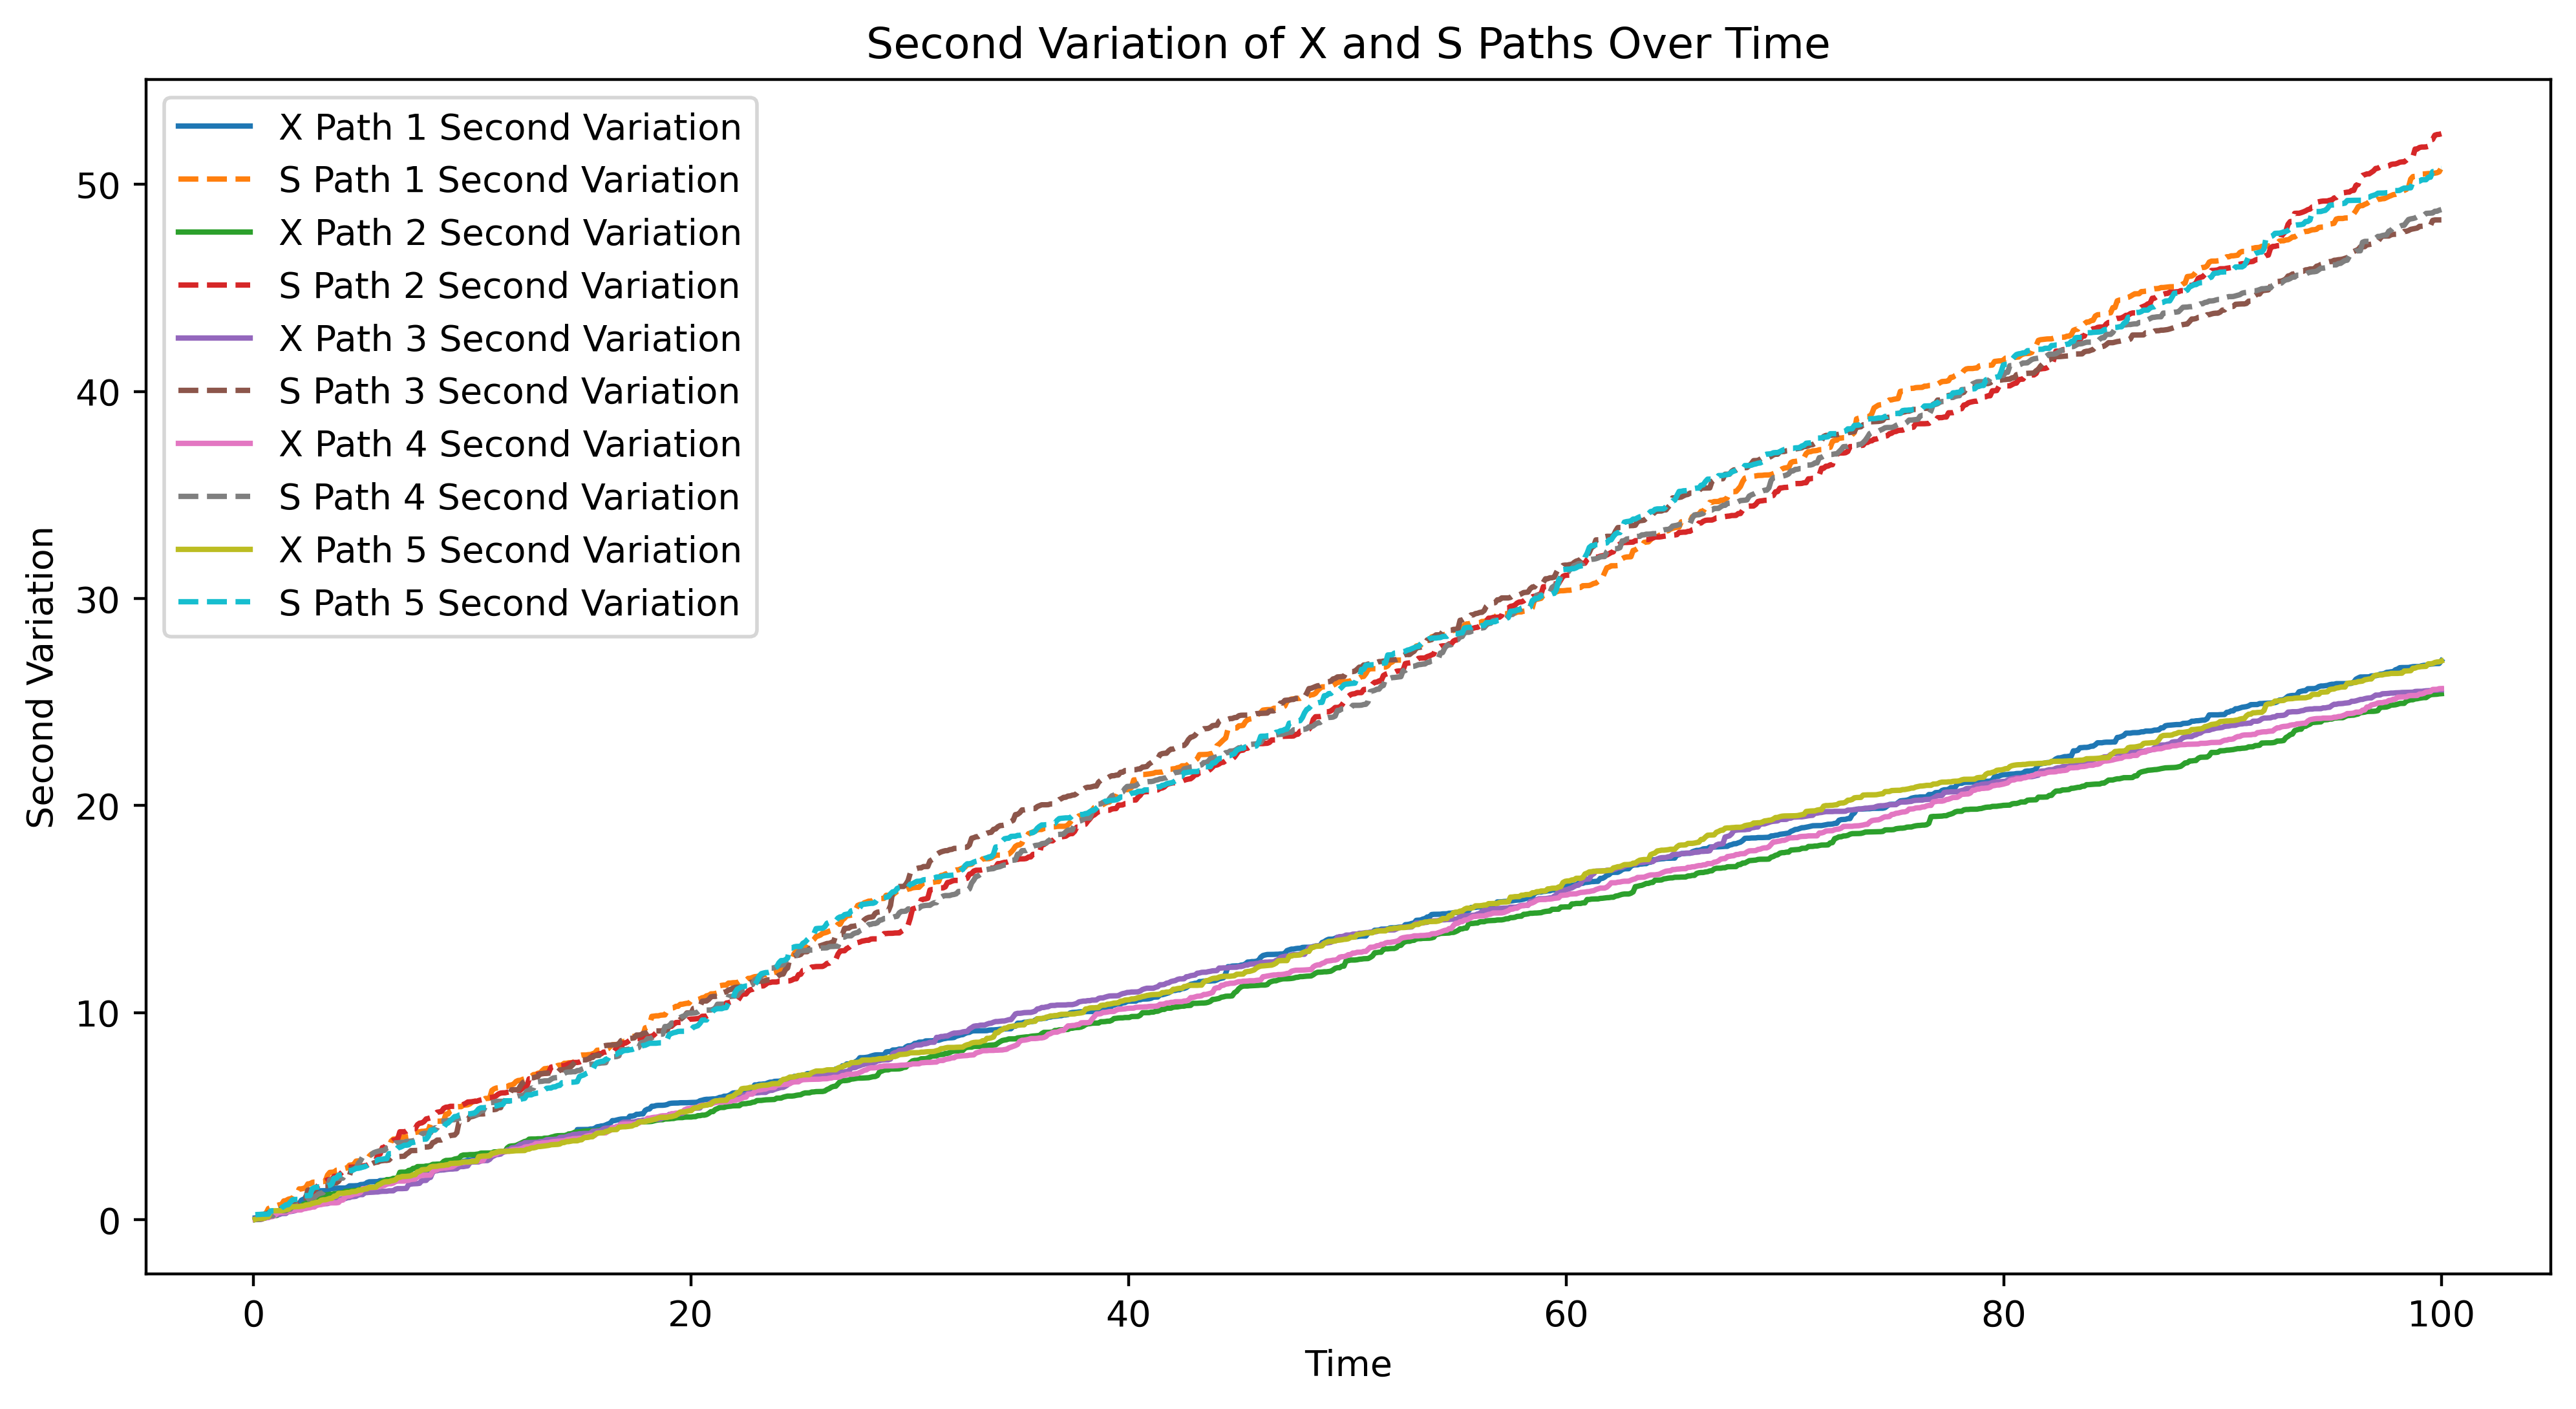
\includegraphics[width=.47\textwidth]{figures/XS3_2d.png}}
    }
    \centering
    \subfigure[模拟$X_t$和$S_t$轨道]
    {
        {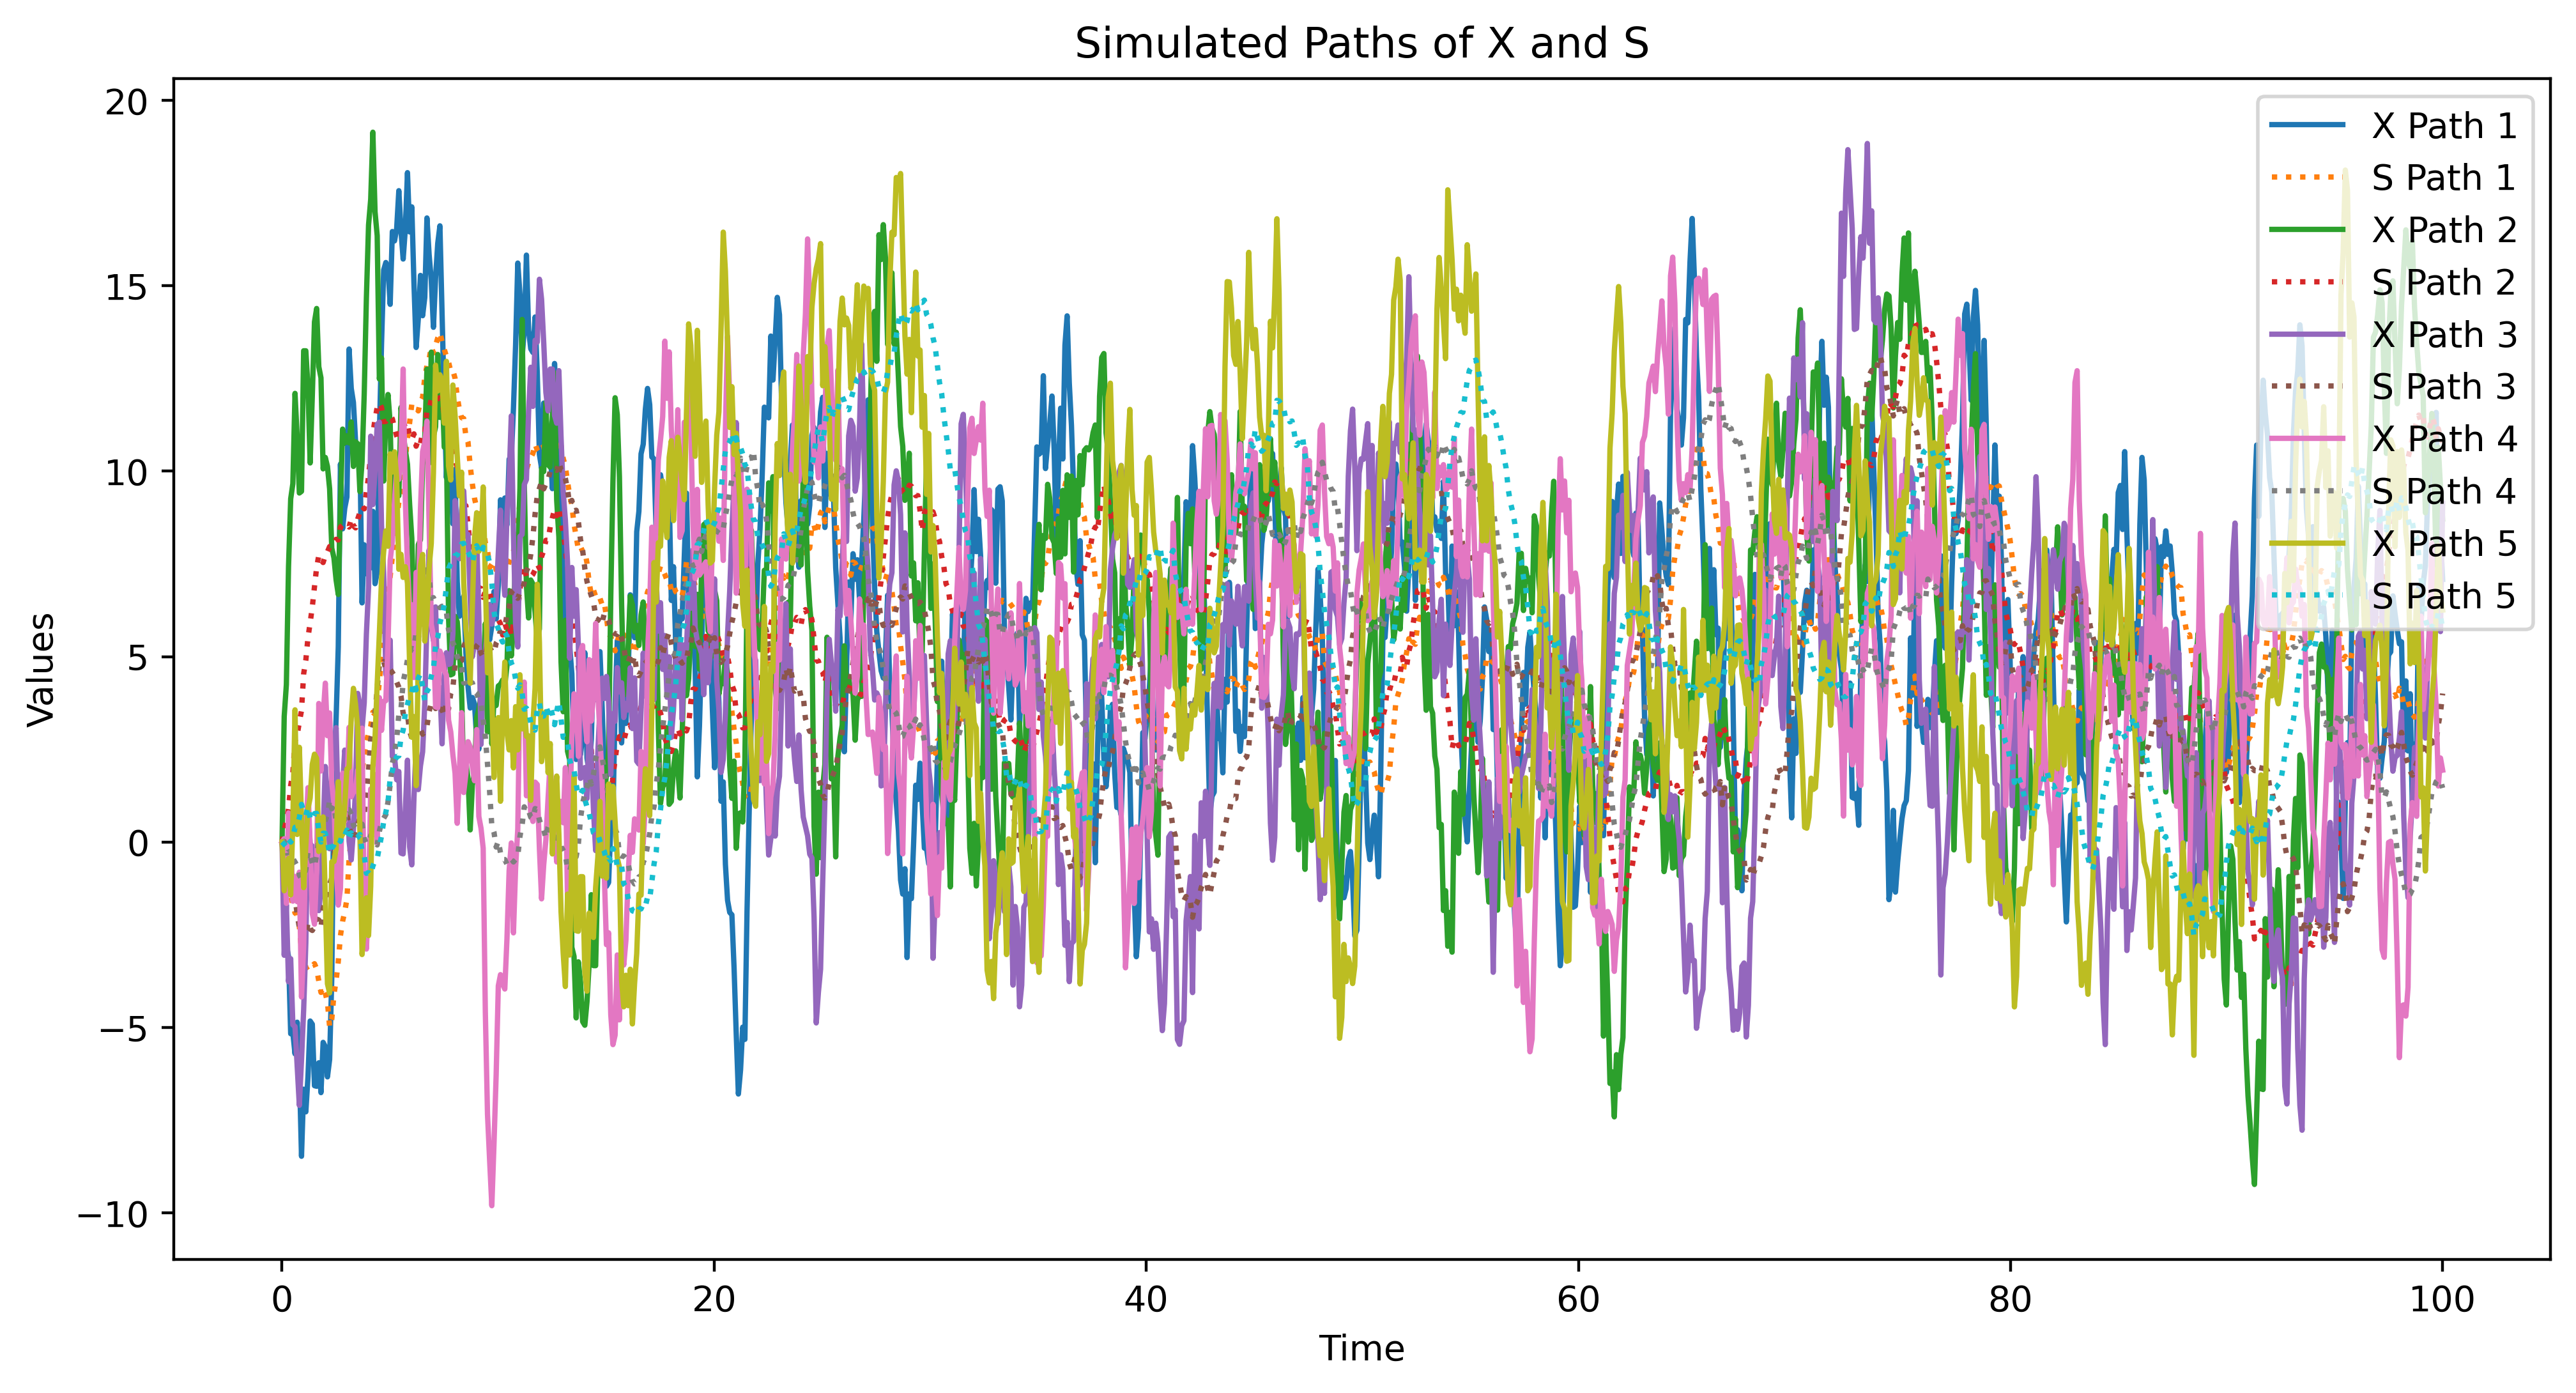
\includegraphics[width=.47\textwidth]{figures/XS4.png}}
    }
    \subfigure[模拟$X_t$和$S_t$轨道2阶变差]
    {
        {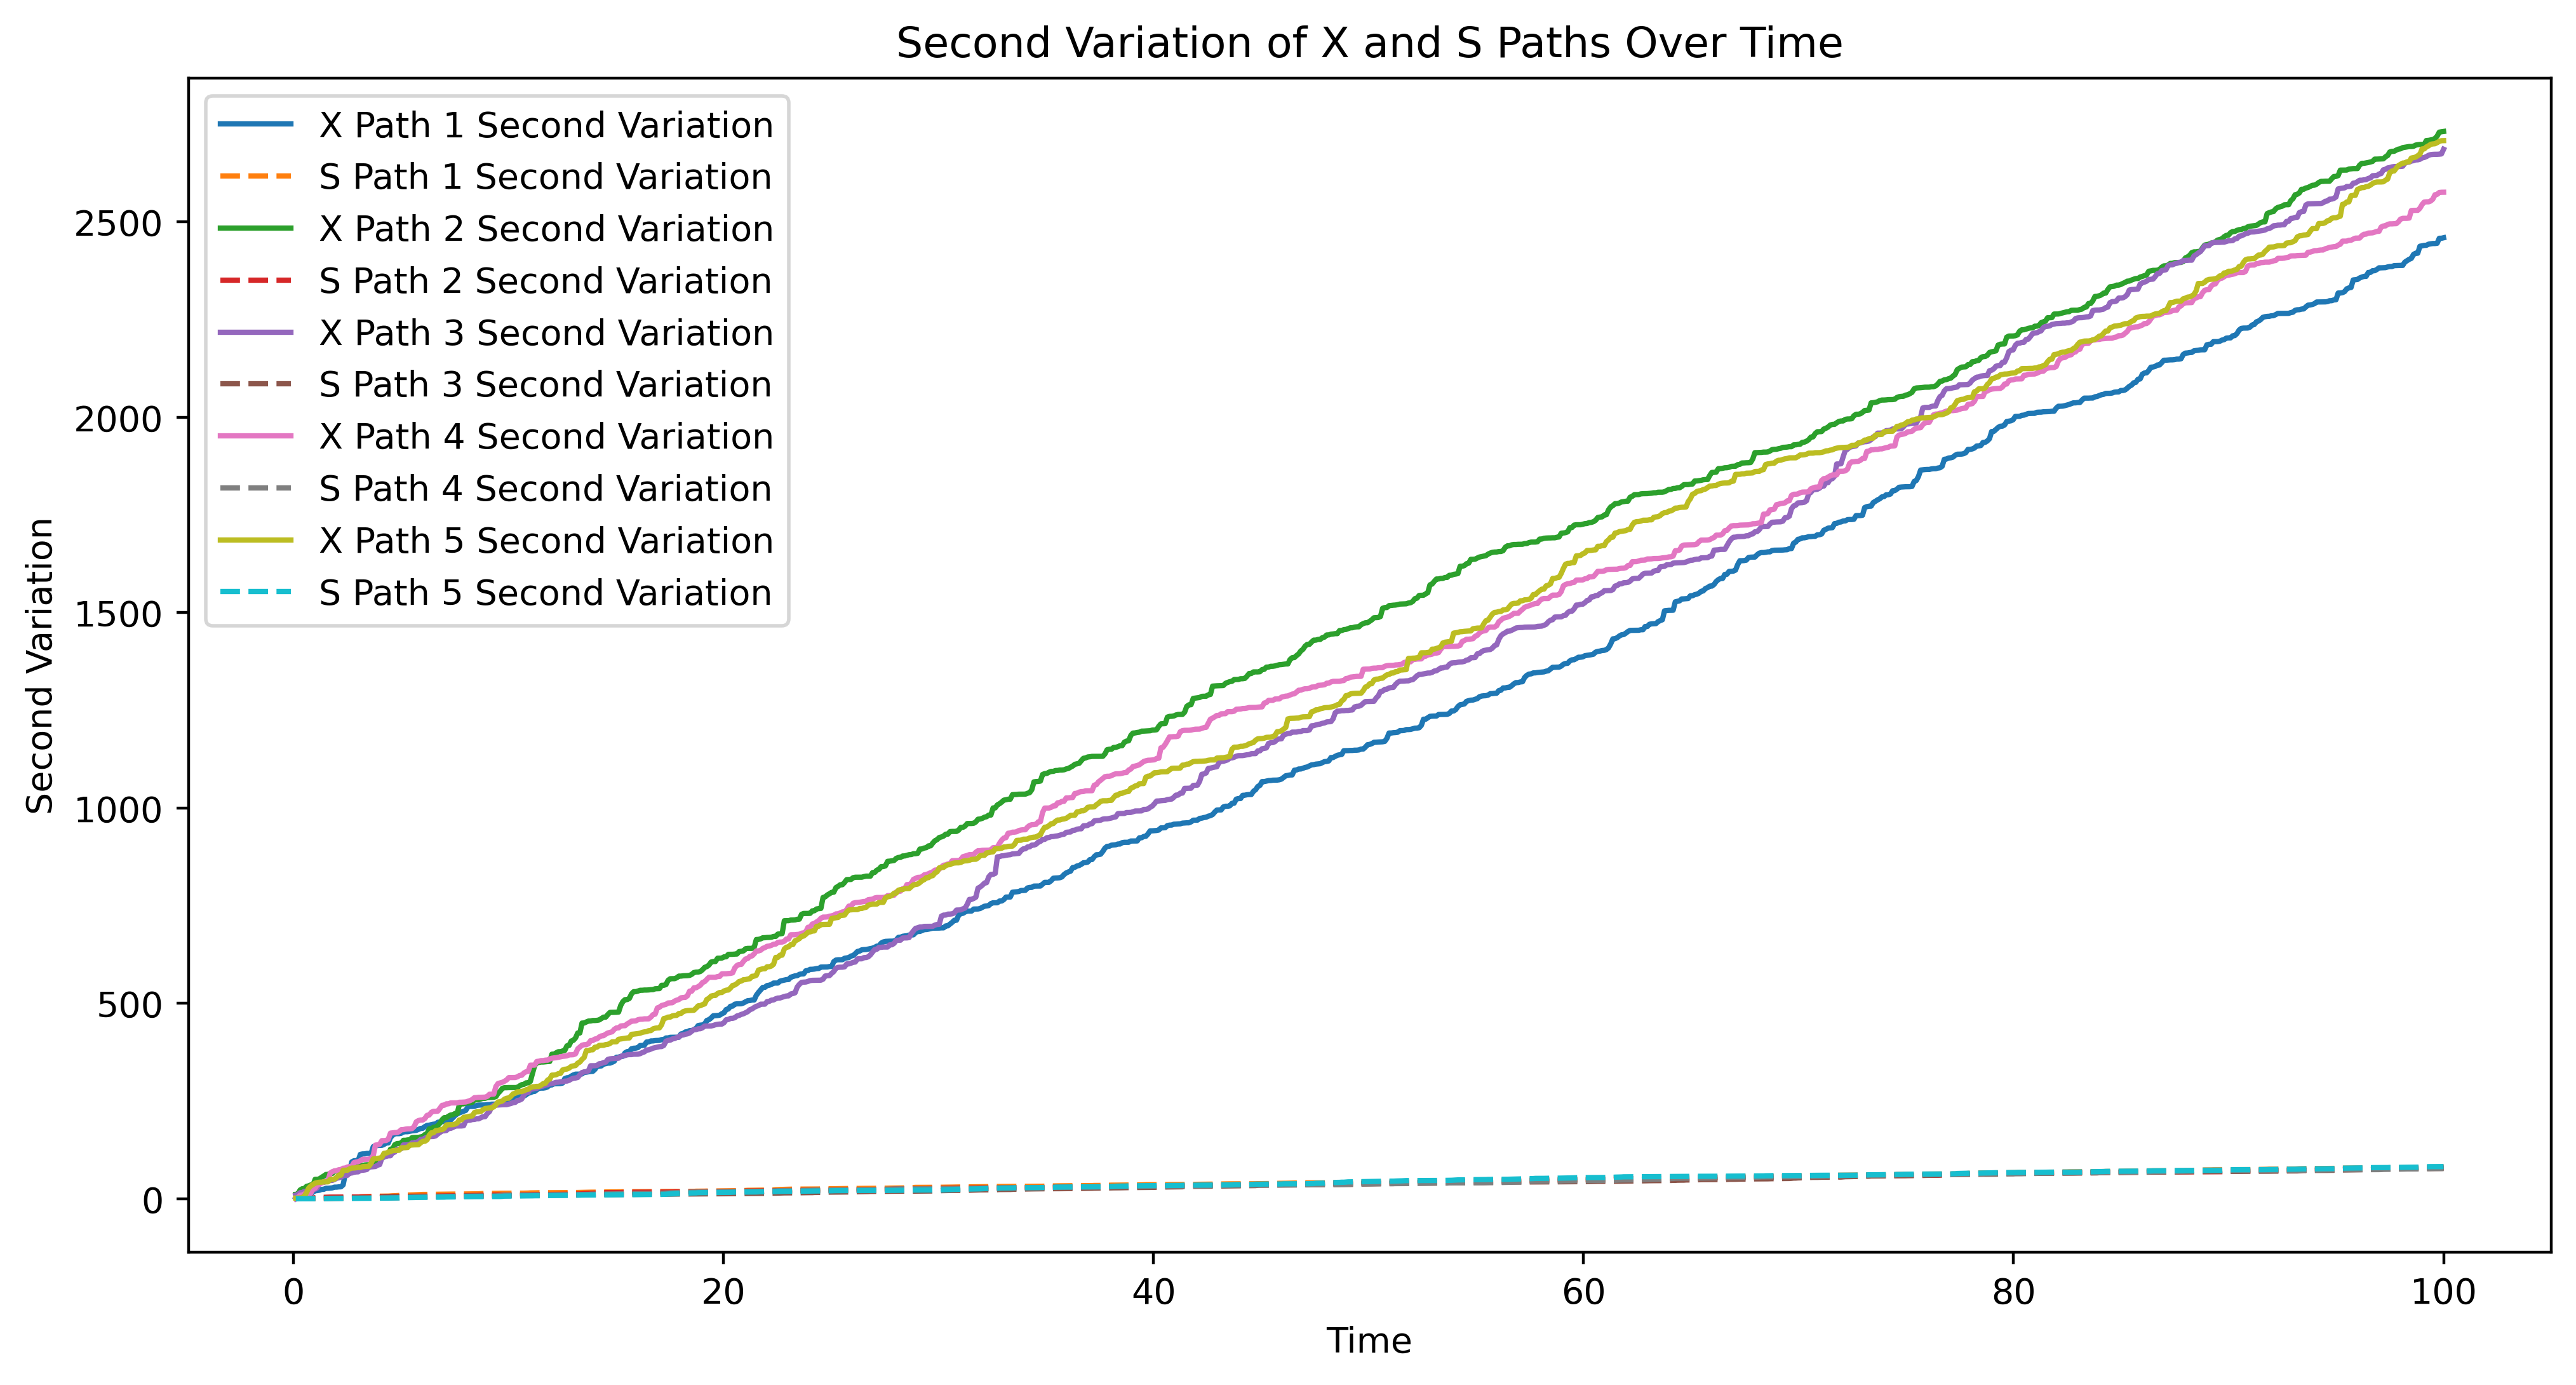
\includegraphics[width=.47\textwidth]{figures/XS4_2d.png}}
    }
 
\caption{对应不同参数的$X_t$和$S_t$}
\label{fig:X_S}
\end{figure}

\begin{figure}[p]
\ContinuedFloat
   \centering
    \subfigure[模拟$X_t$和$S_t$轨道]
    {
        {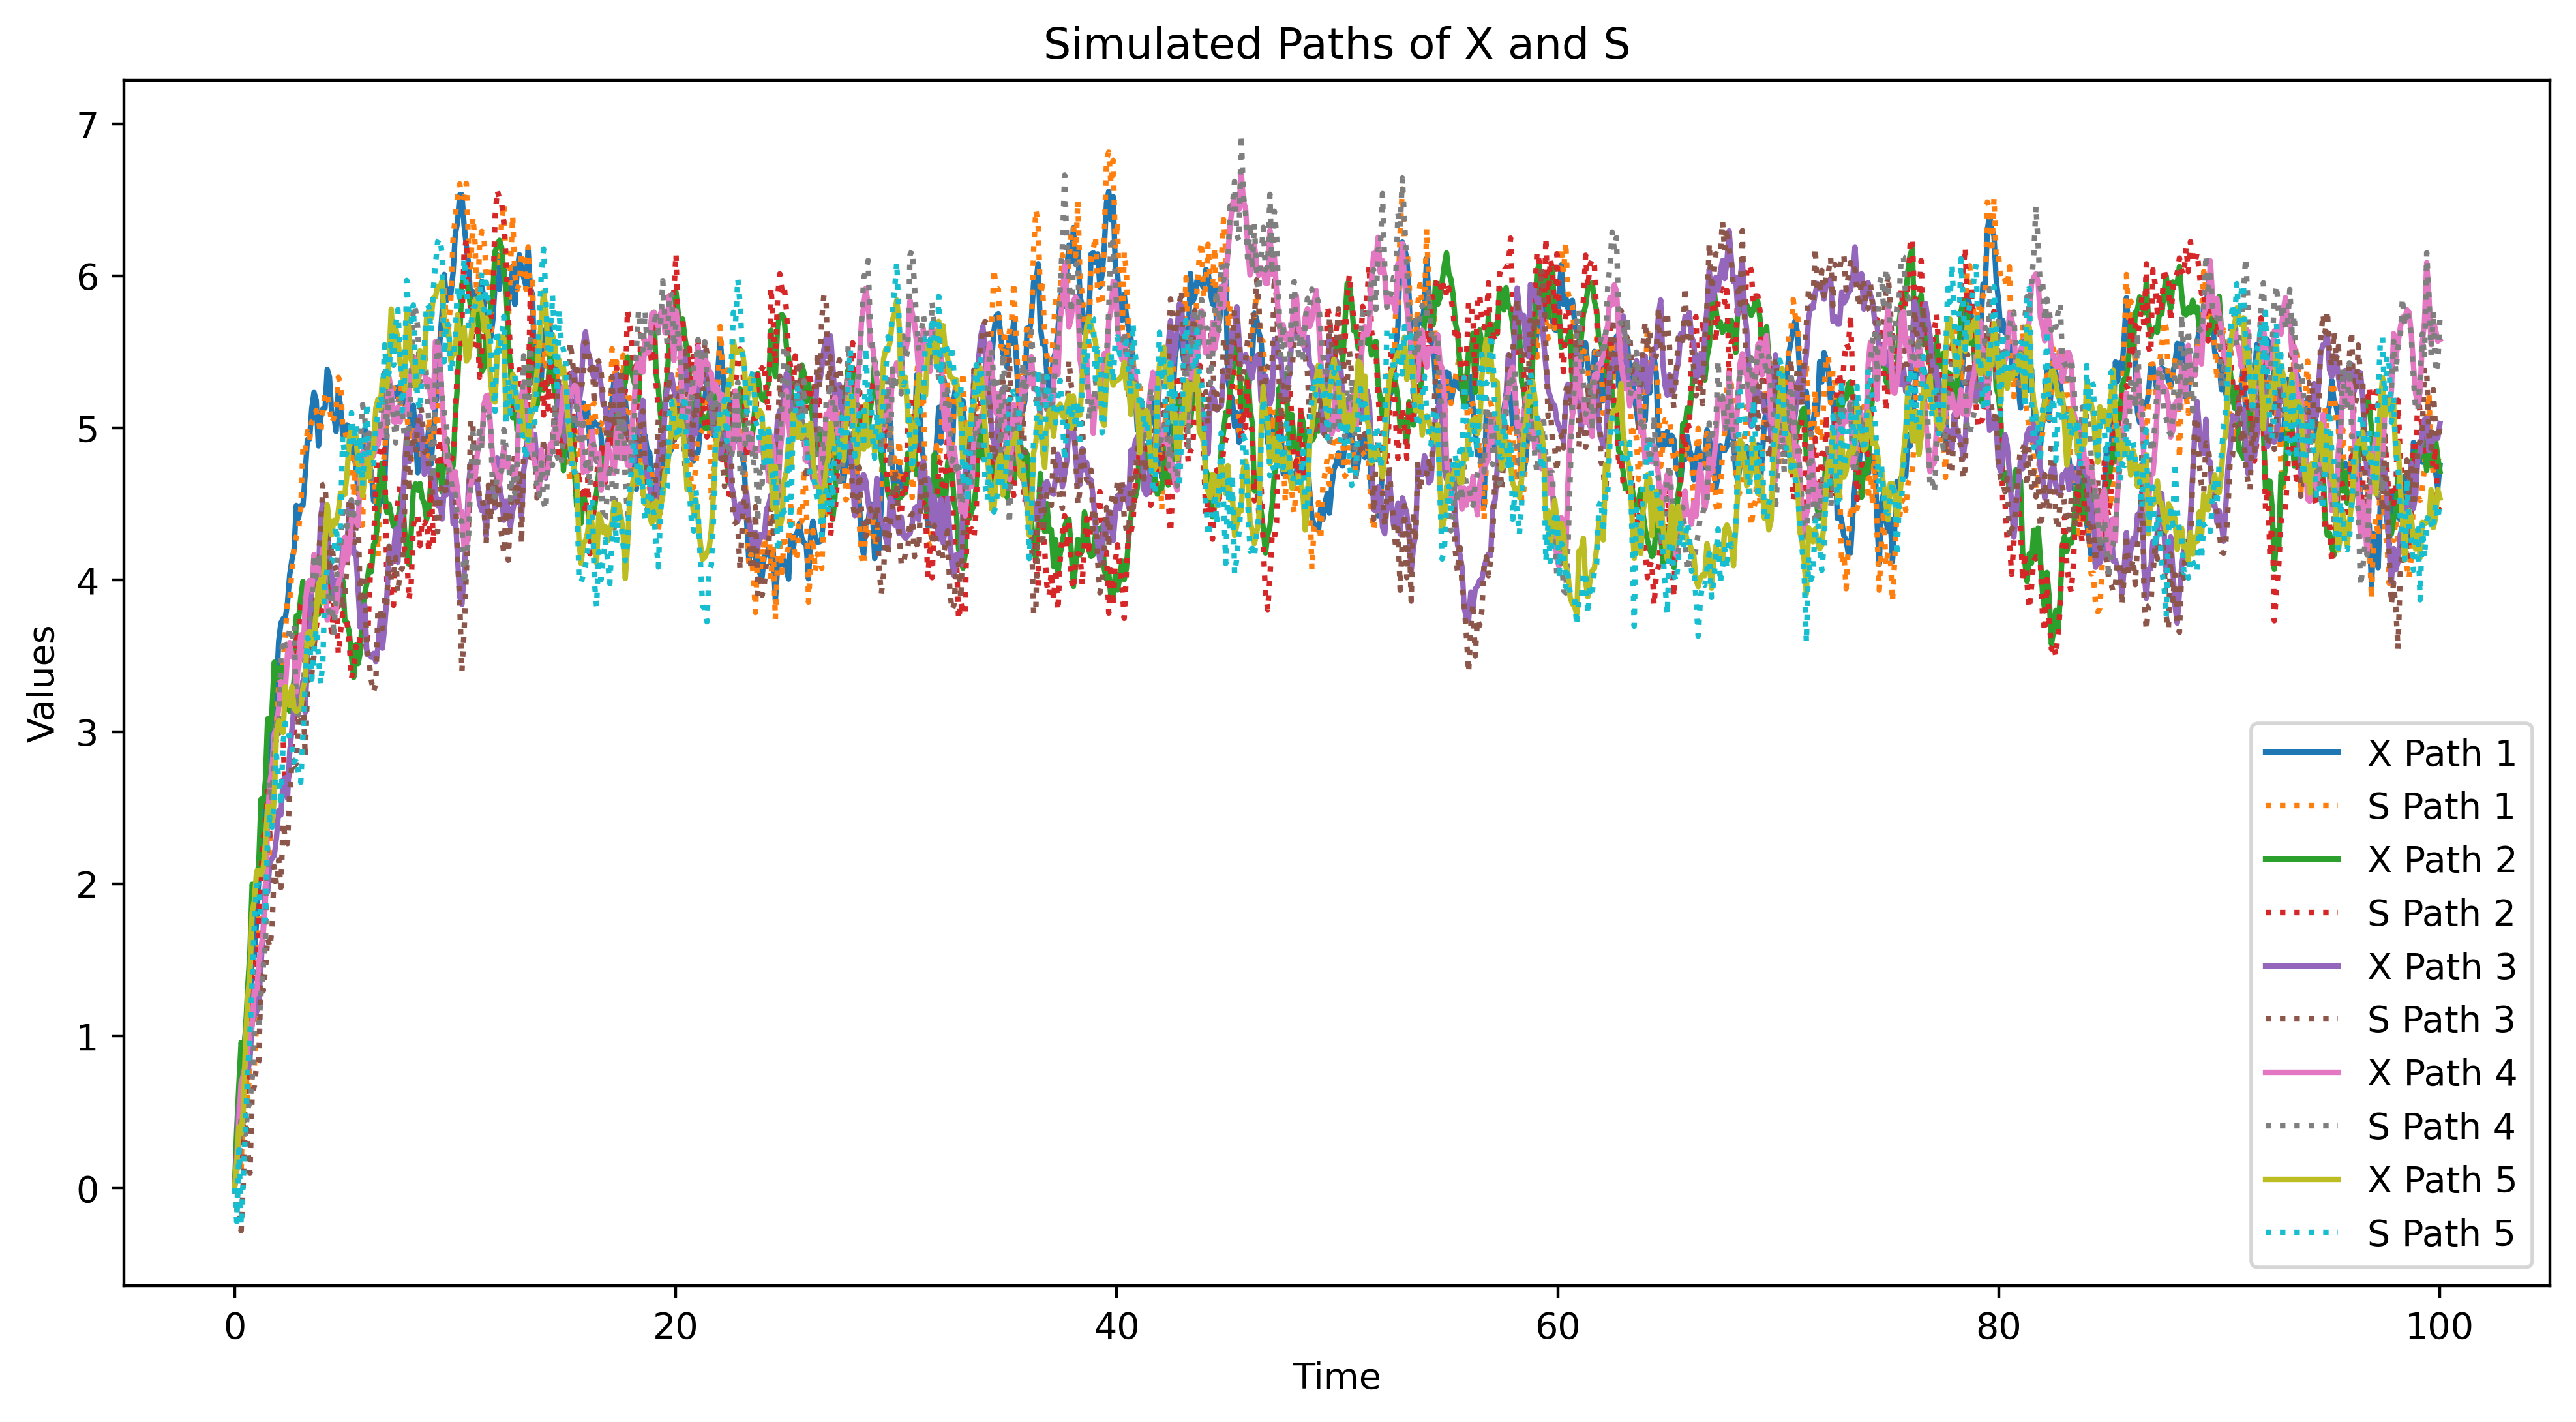
\includegraphics[width=.47\textwidth]{figures/XS5.png}}
    }
    \subfigure[模拟$X_t$和$S_t$轨道2阶变差]
    {
        {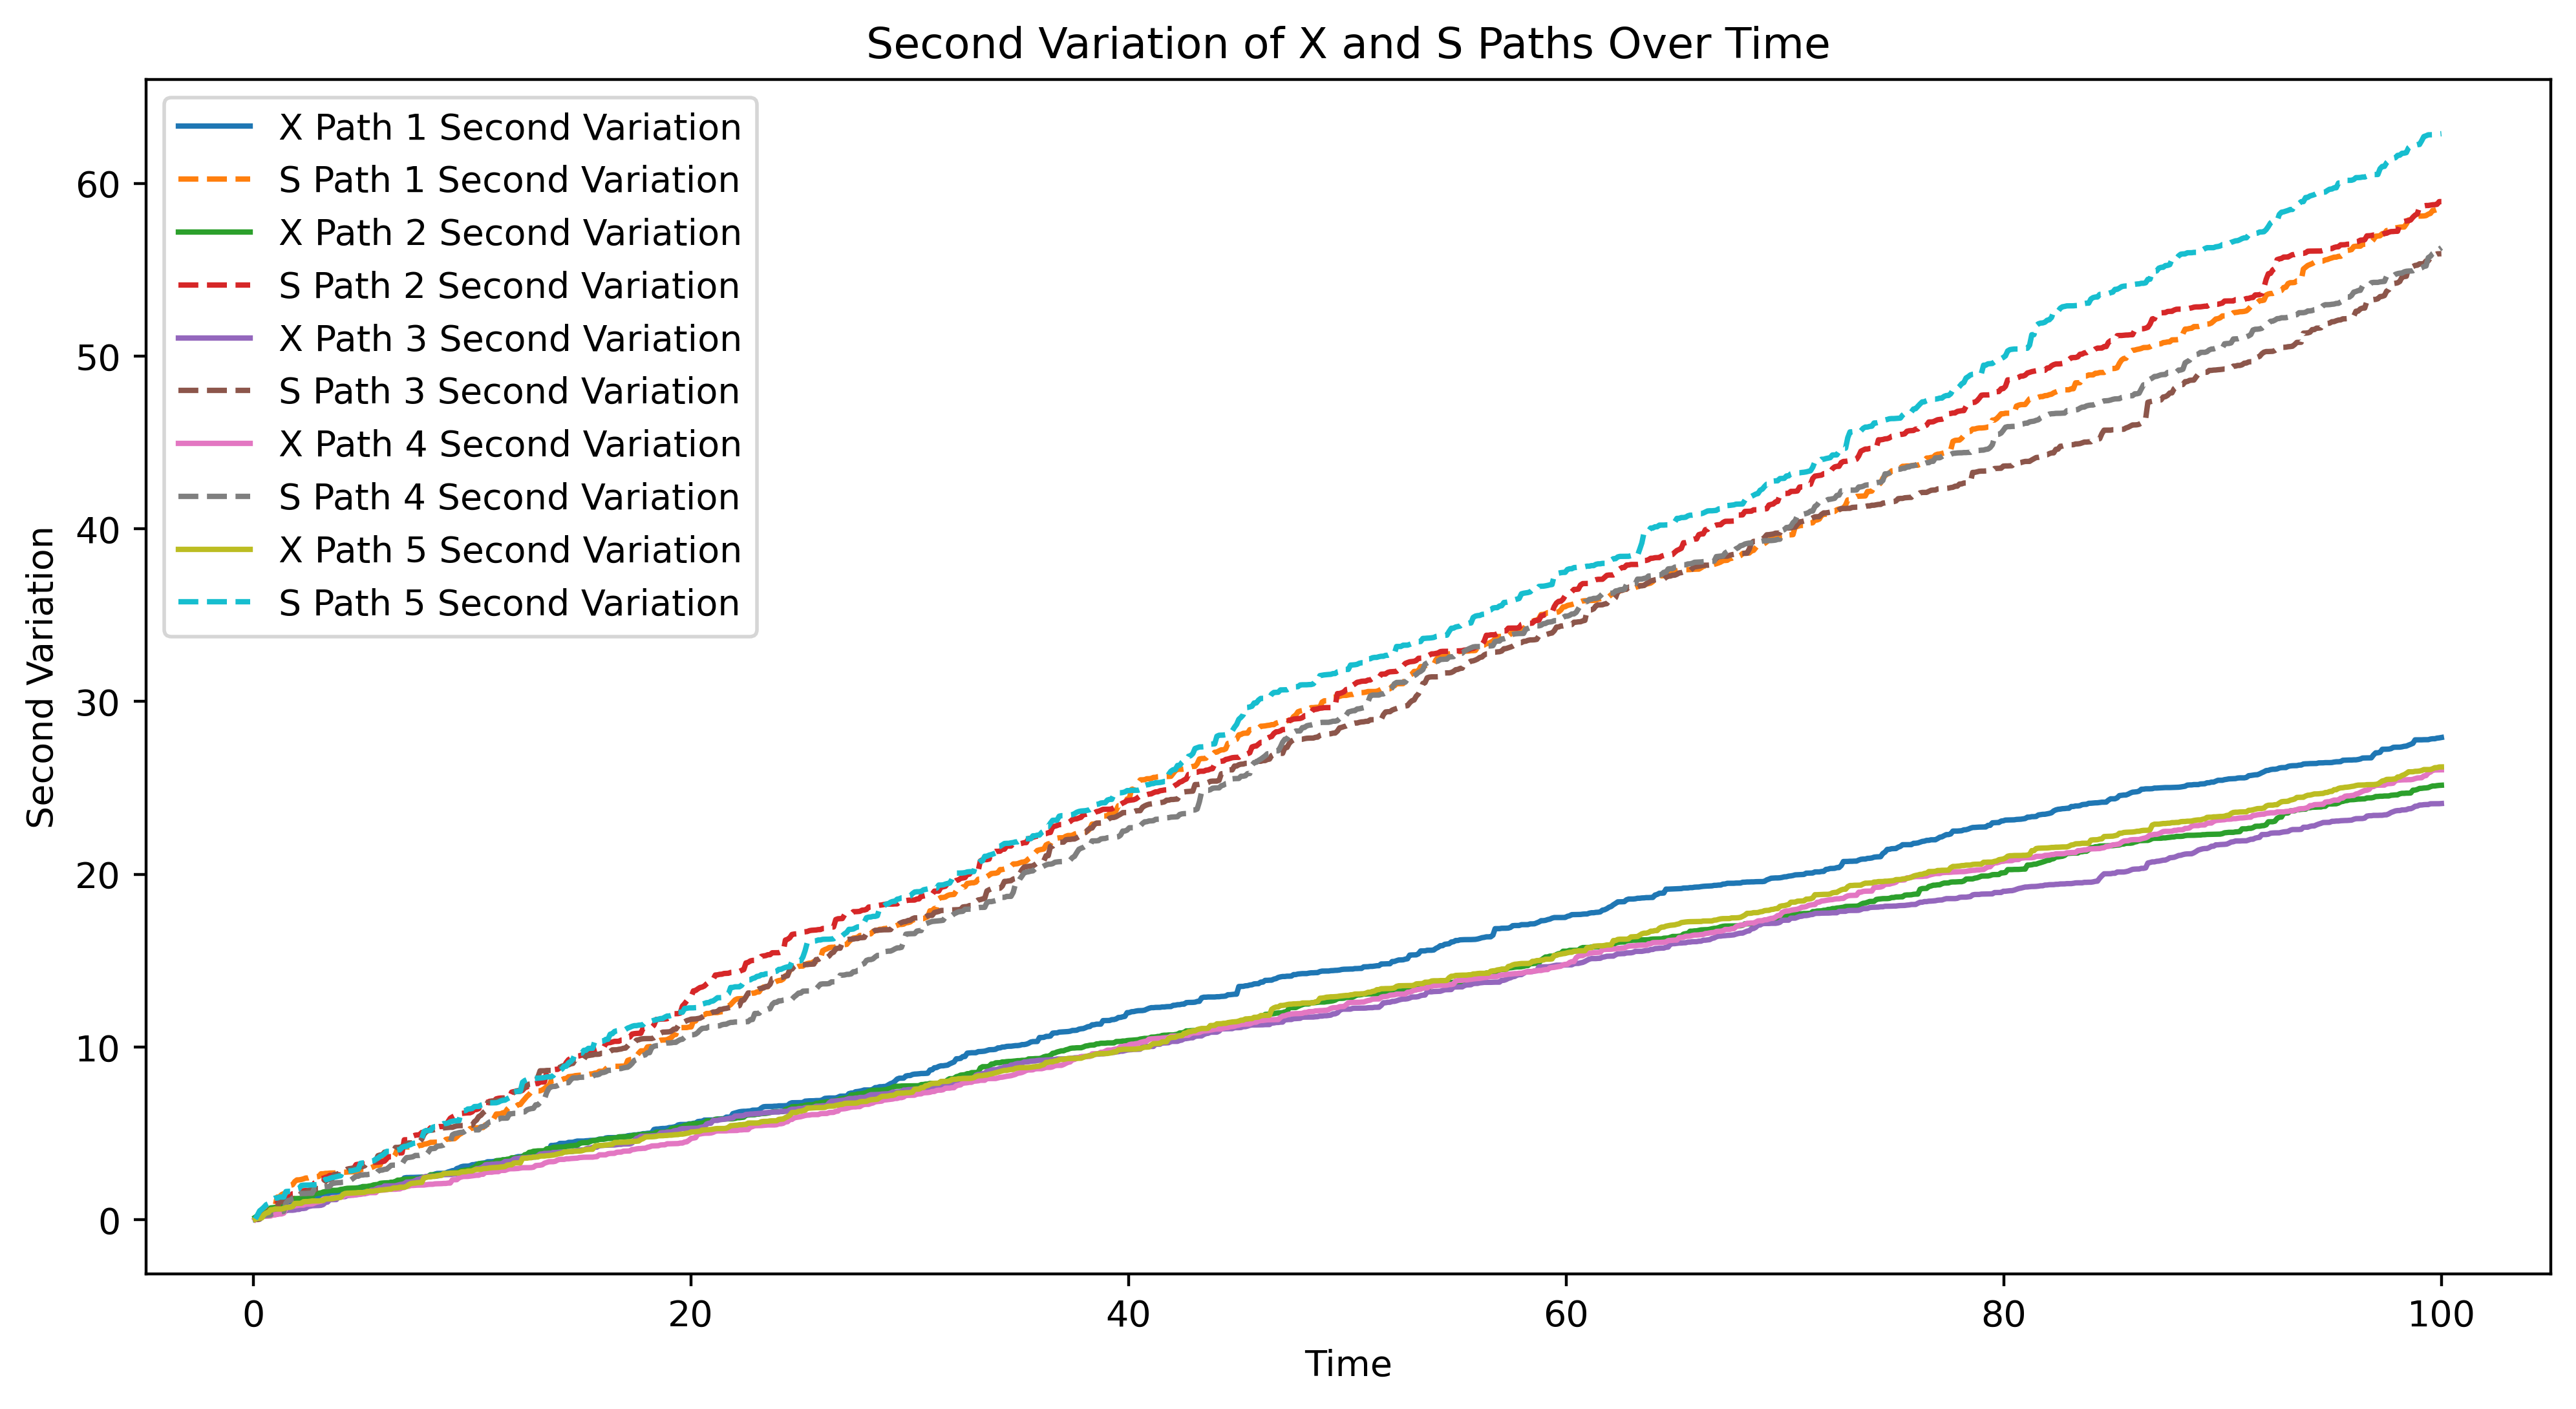
\includegraphics[width=.47\textwidth]{figures/XS5_2d.png}}
    }
    \centering
    \subfigure[模拟$X_t$和$S_t$轨道]
    {
        {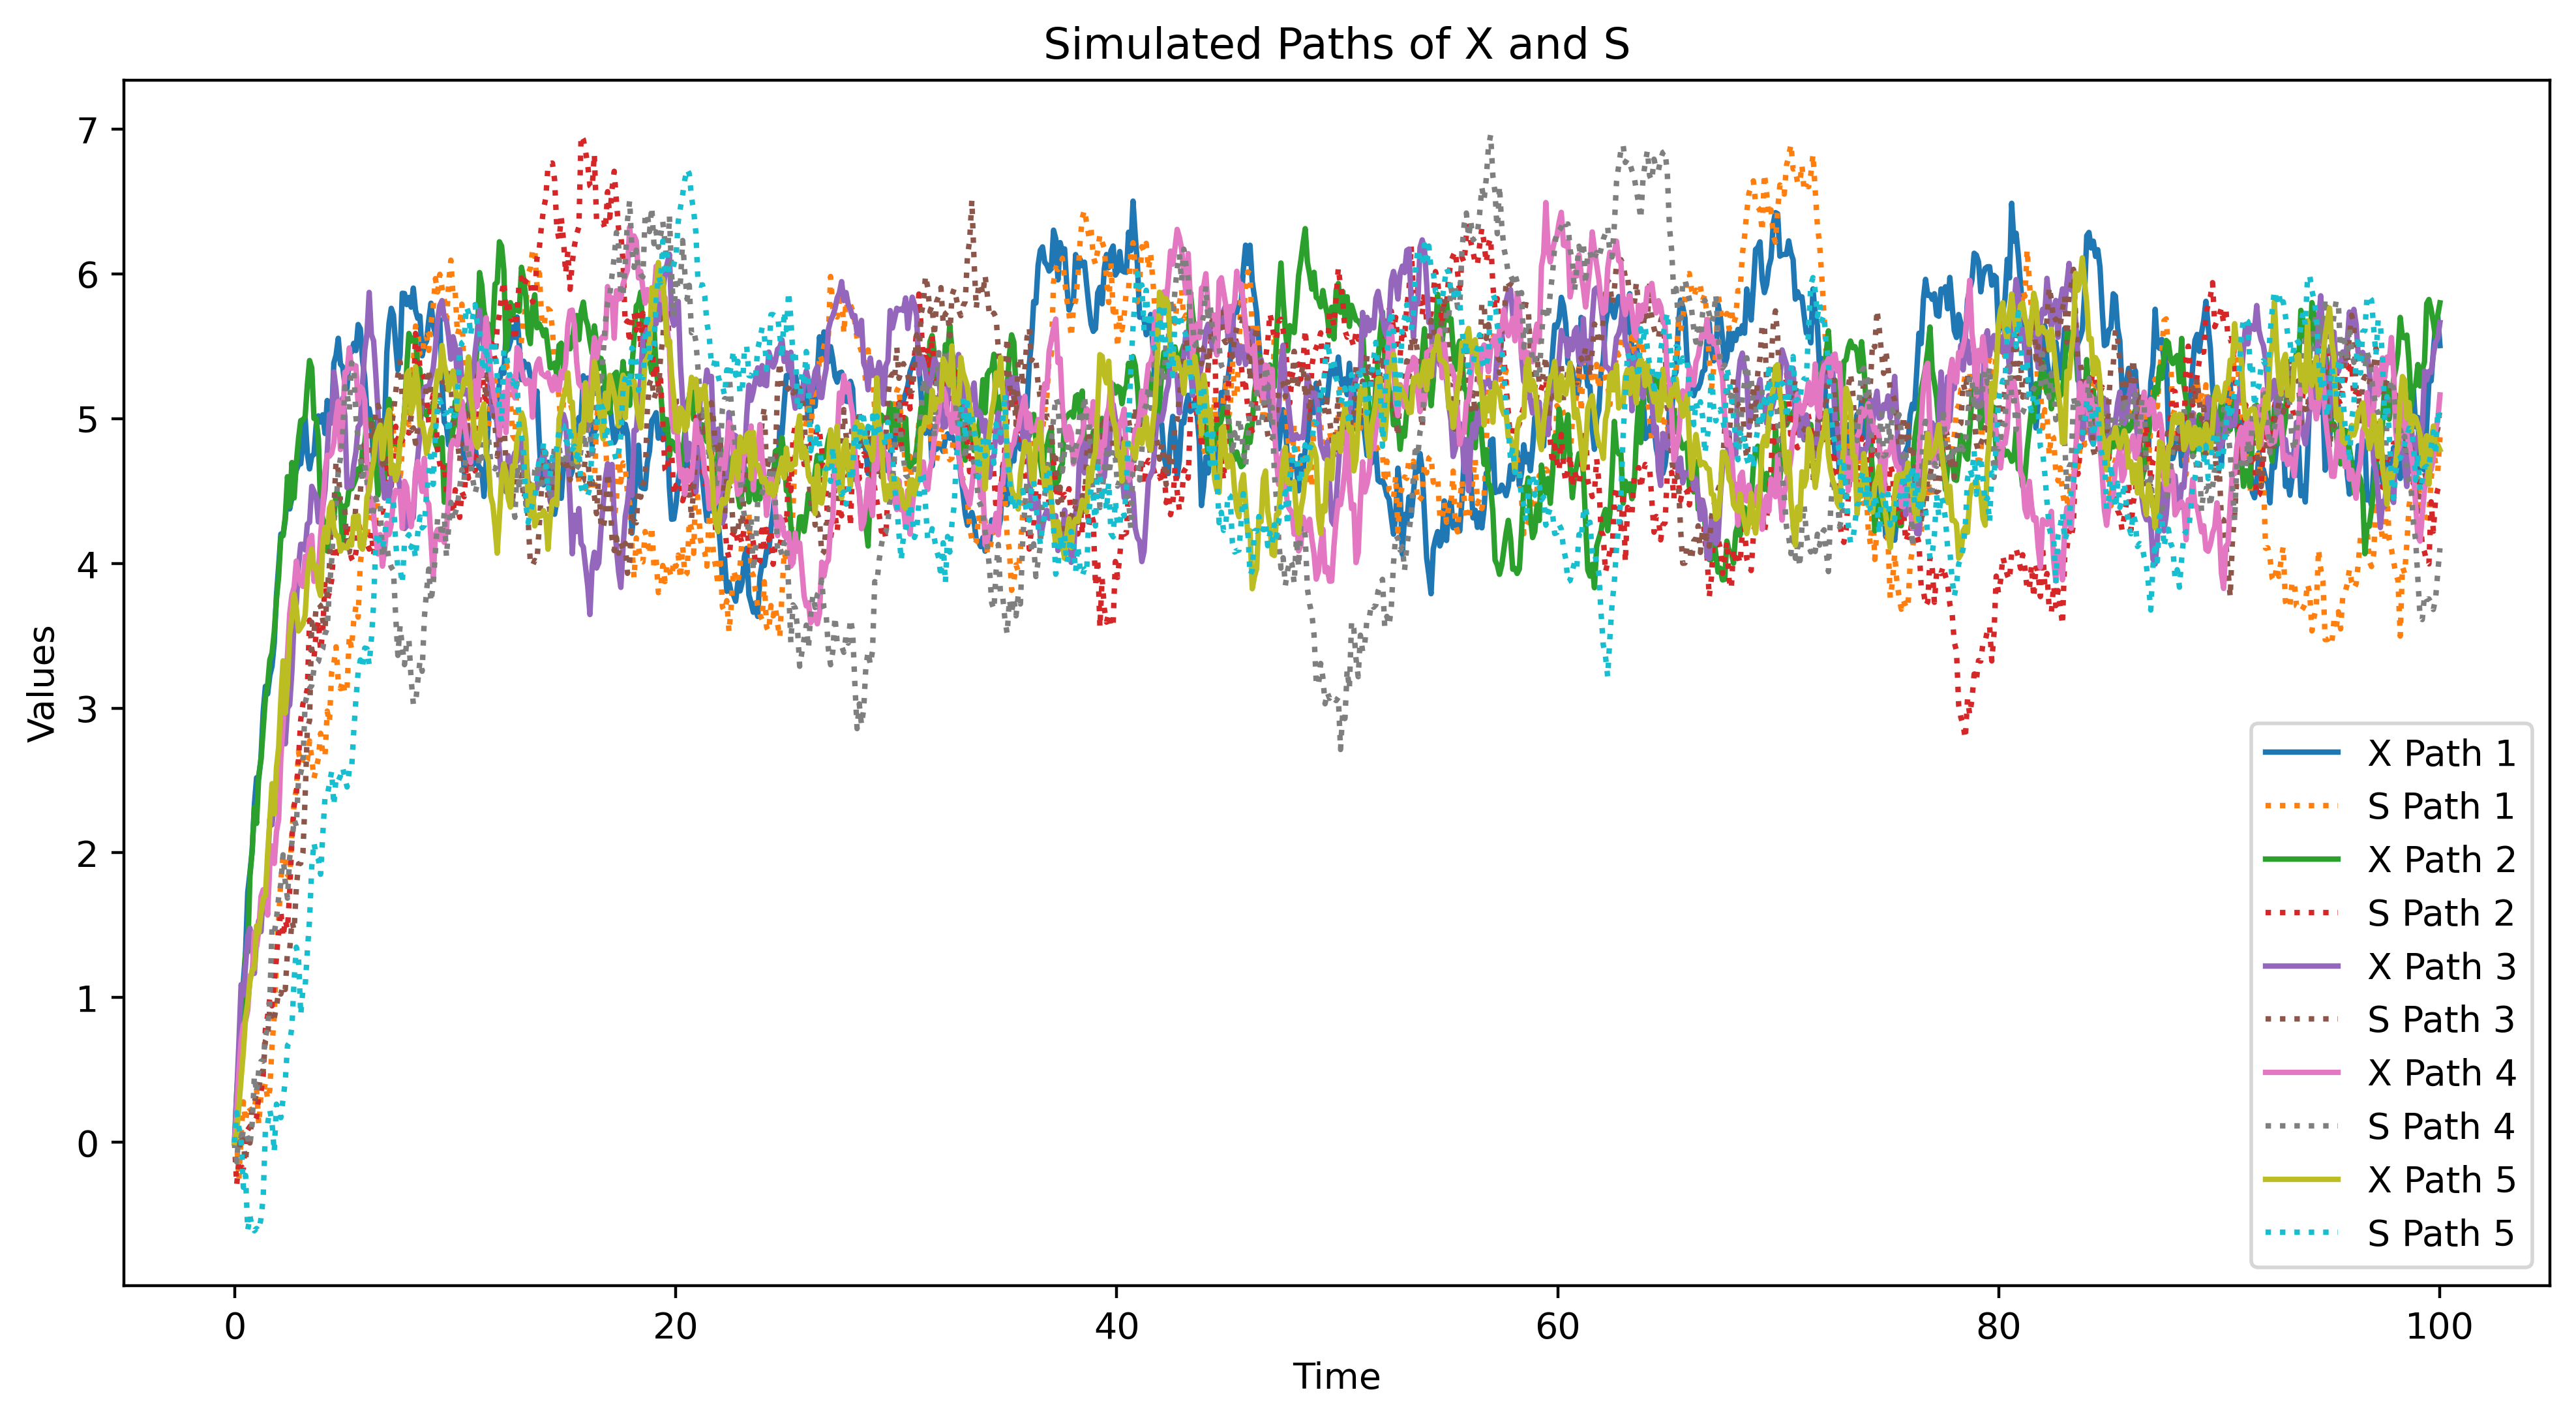
\includegraphics[width=.47\textwidth]{figures/XS6.png}}
    }
    \subfigure[模拟$X_t$和$S_t$轨道2阶变差]
    {
        {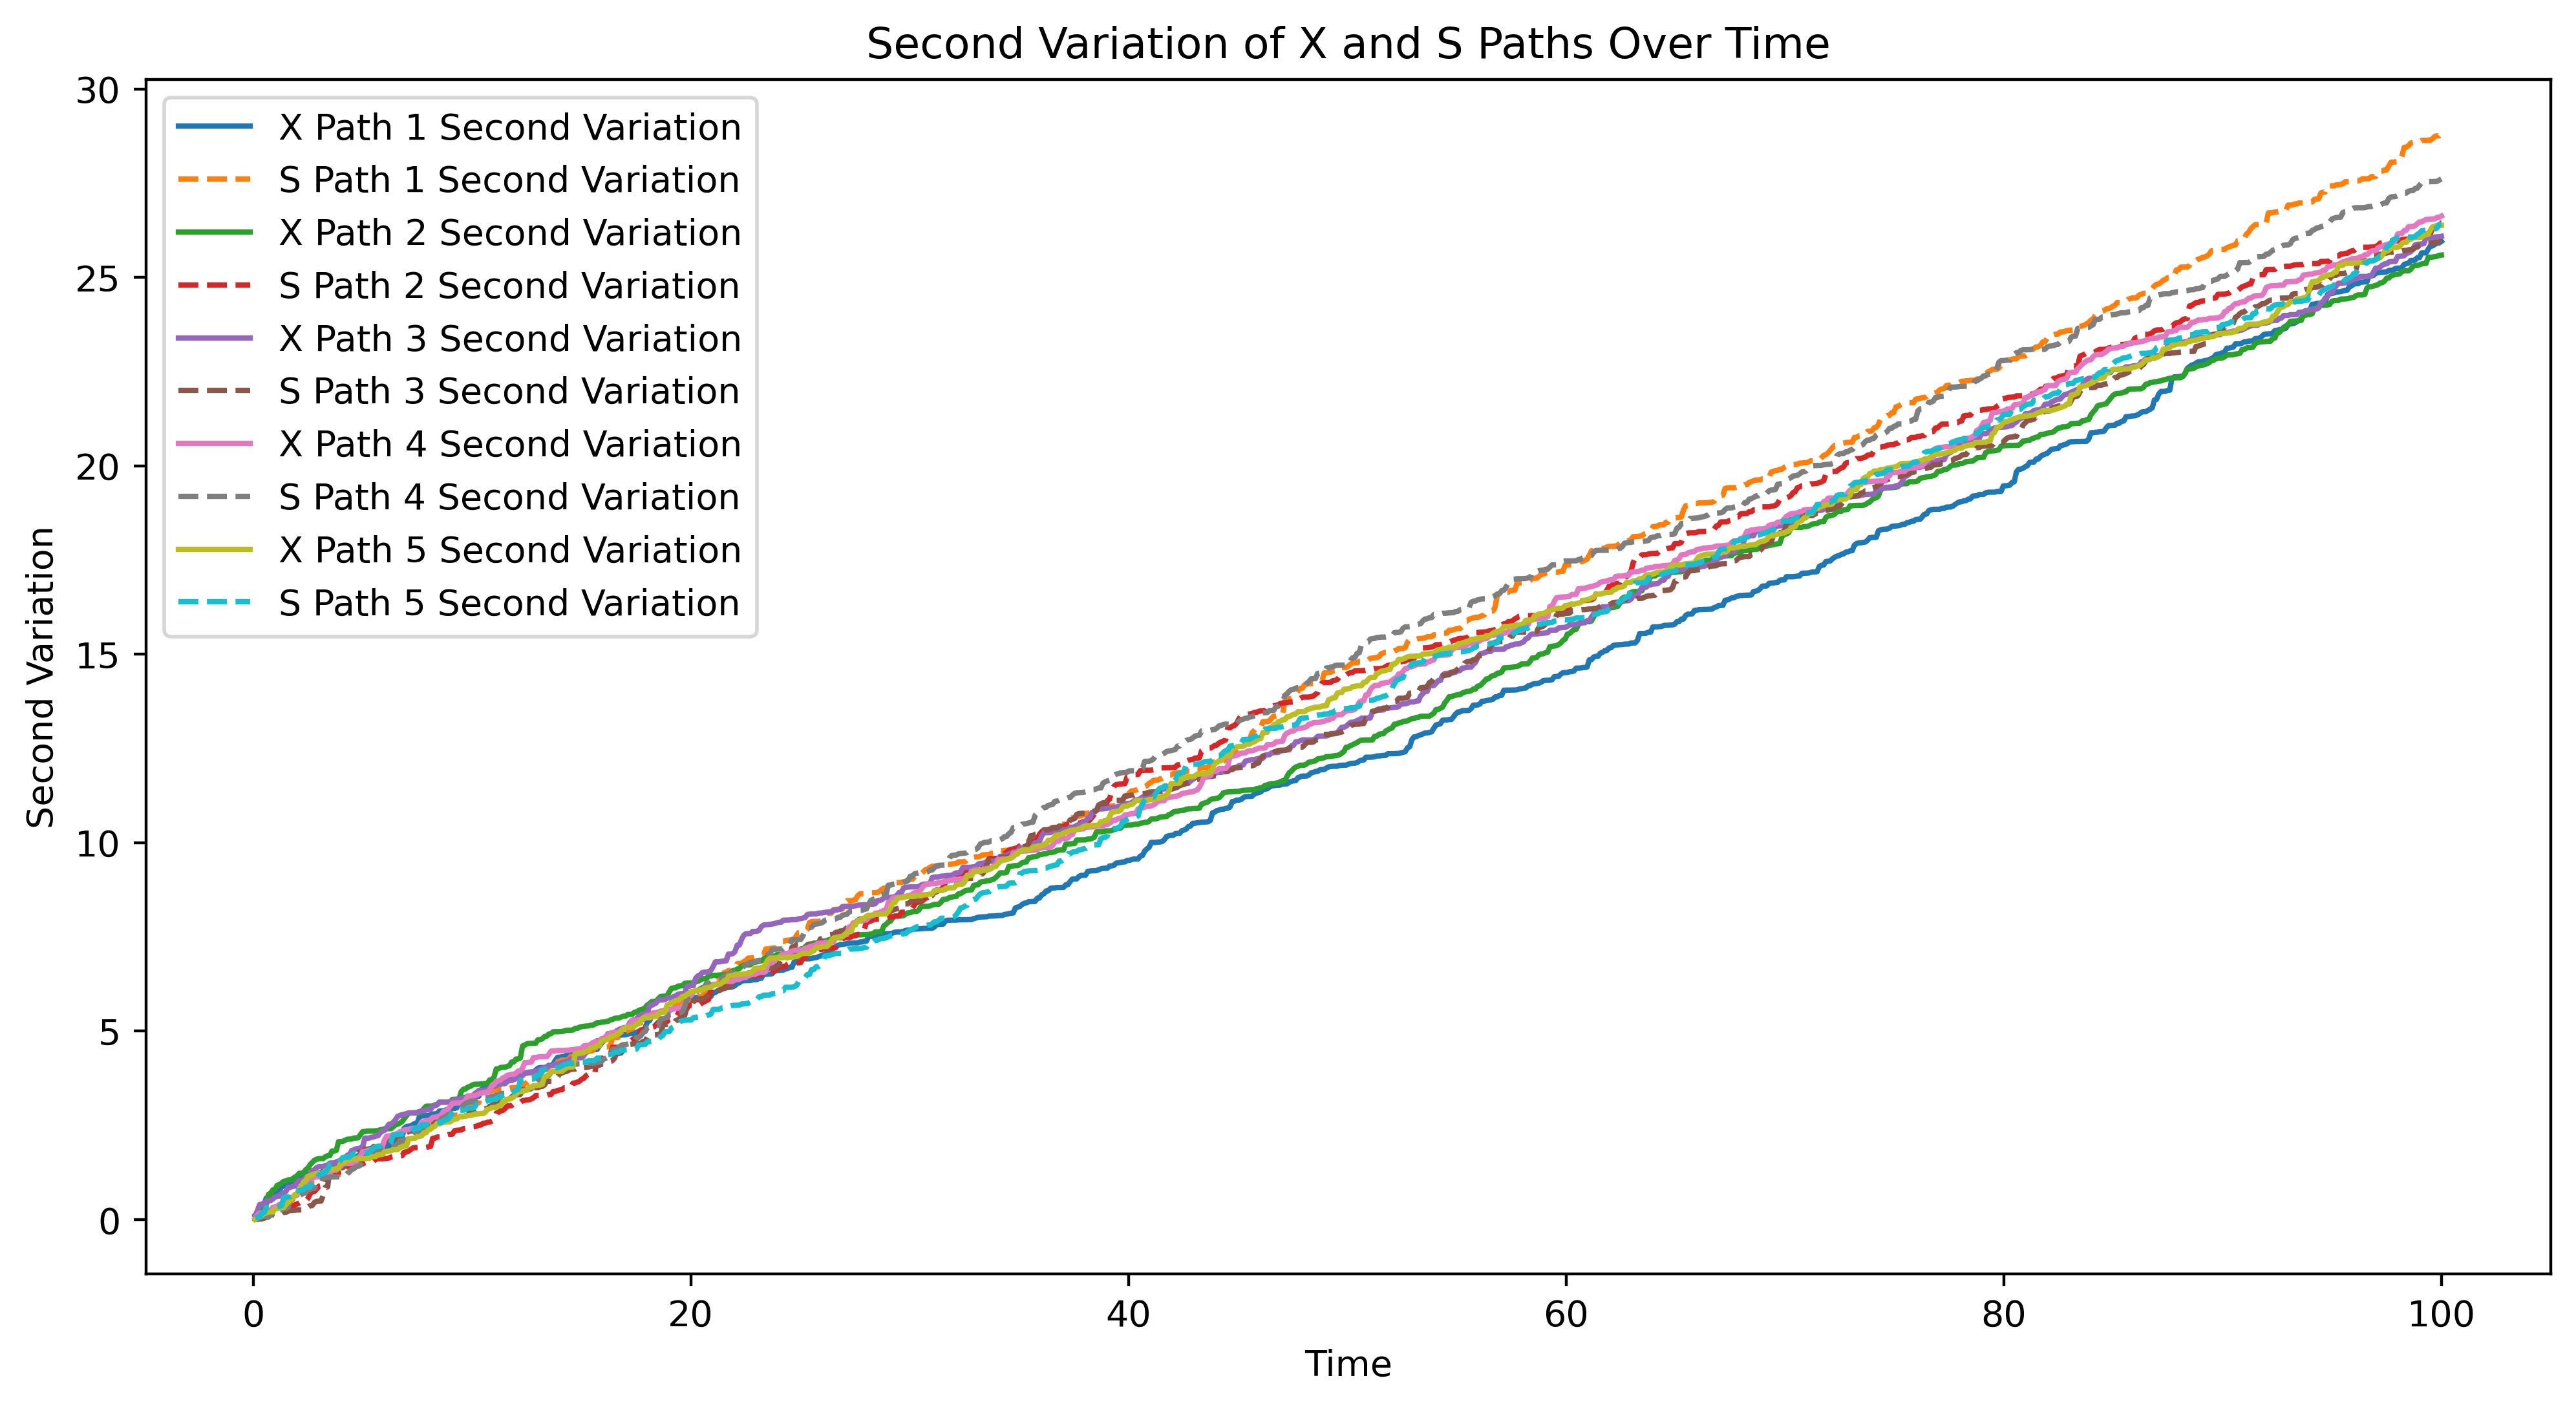
\includegraphics[width=.47\textwidth]{figures/XS6_2d.png}}
    }

    \centering
    \subfigure[模拟$X_t$和$S_t$轨道]
    {
        {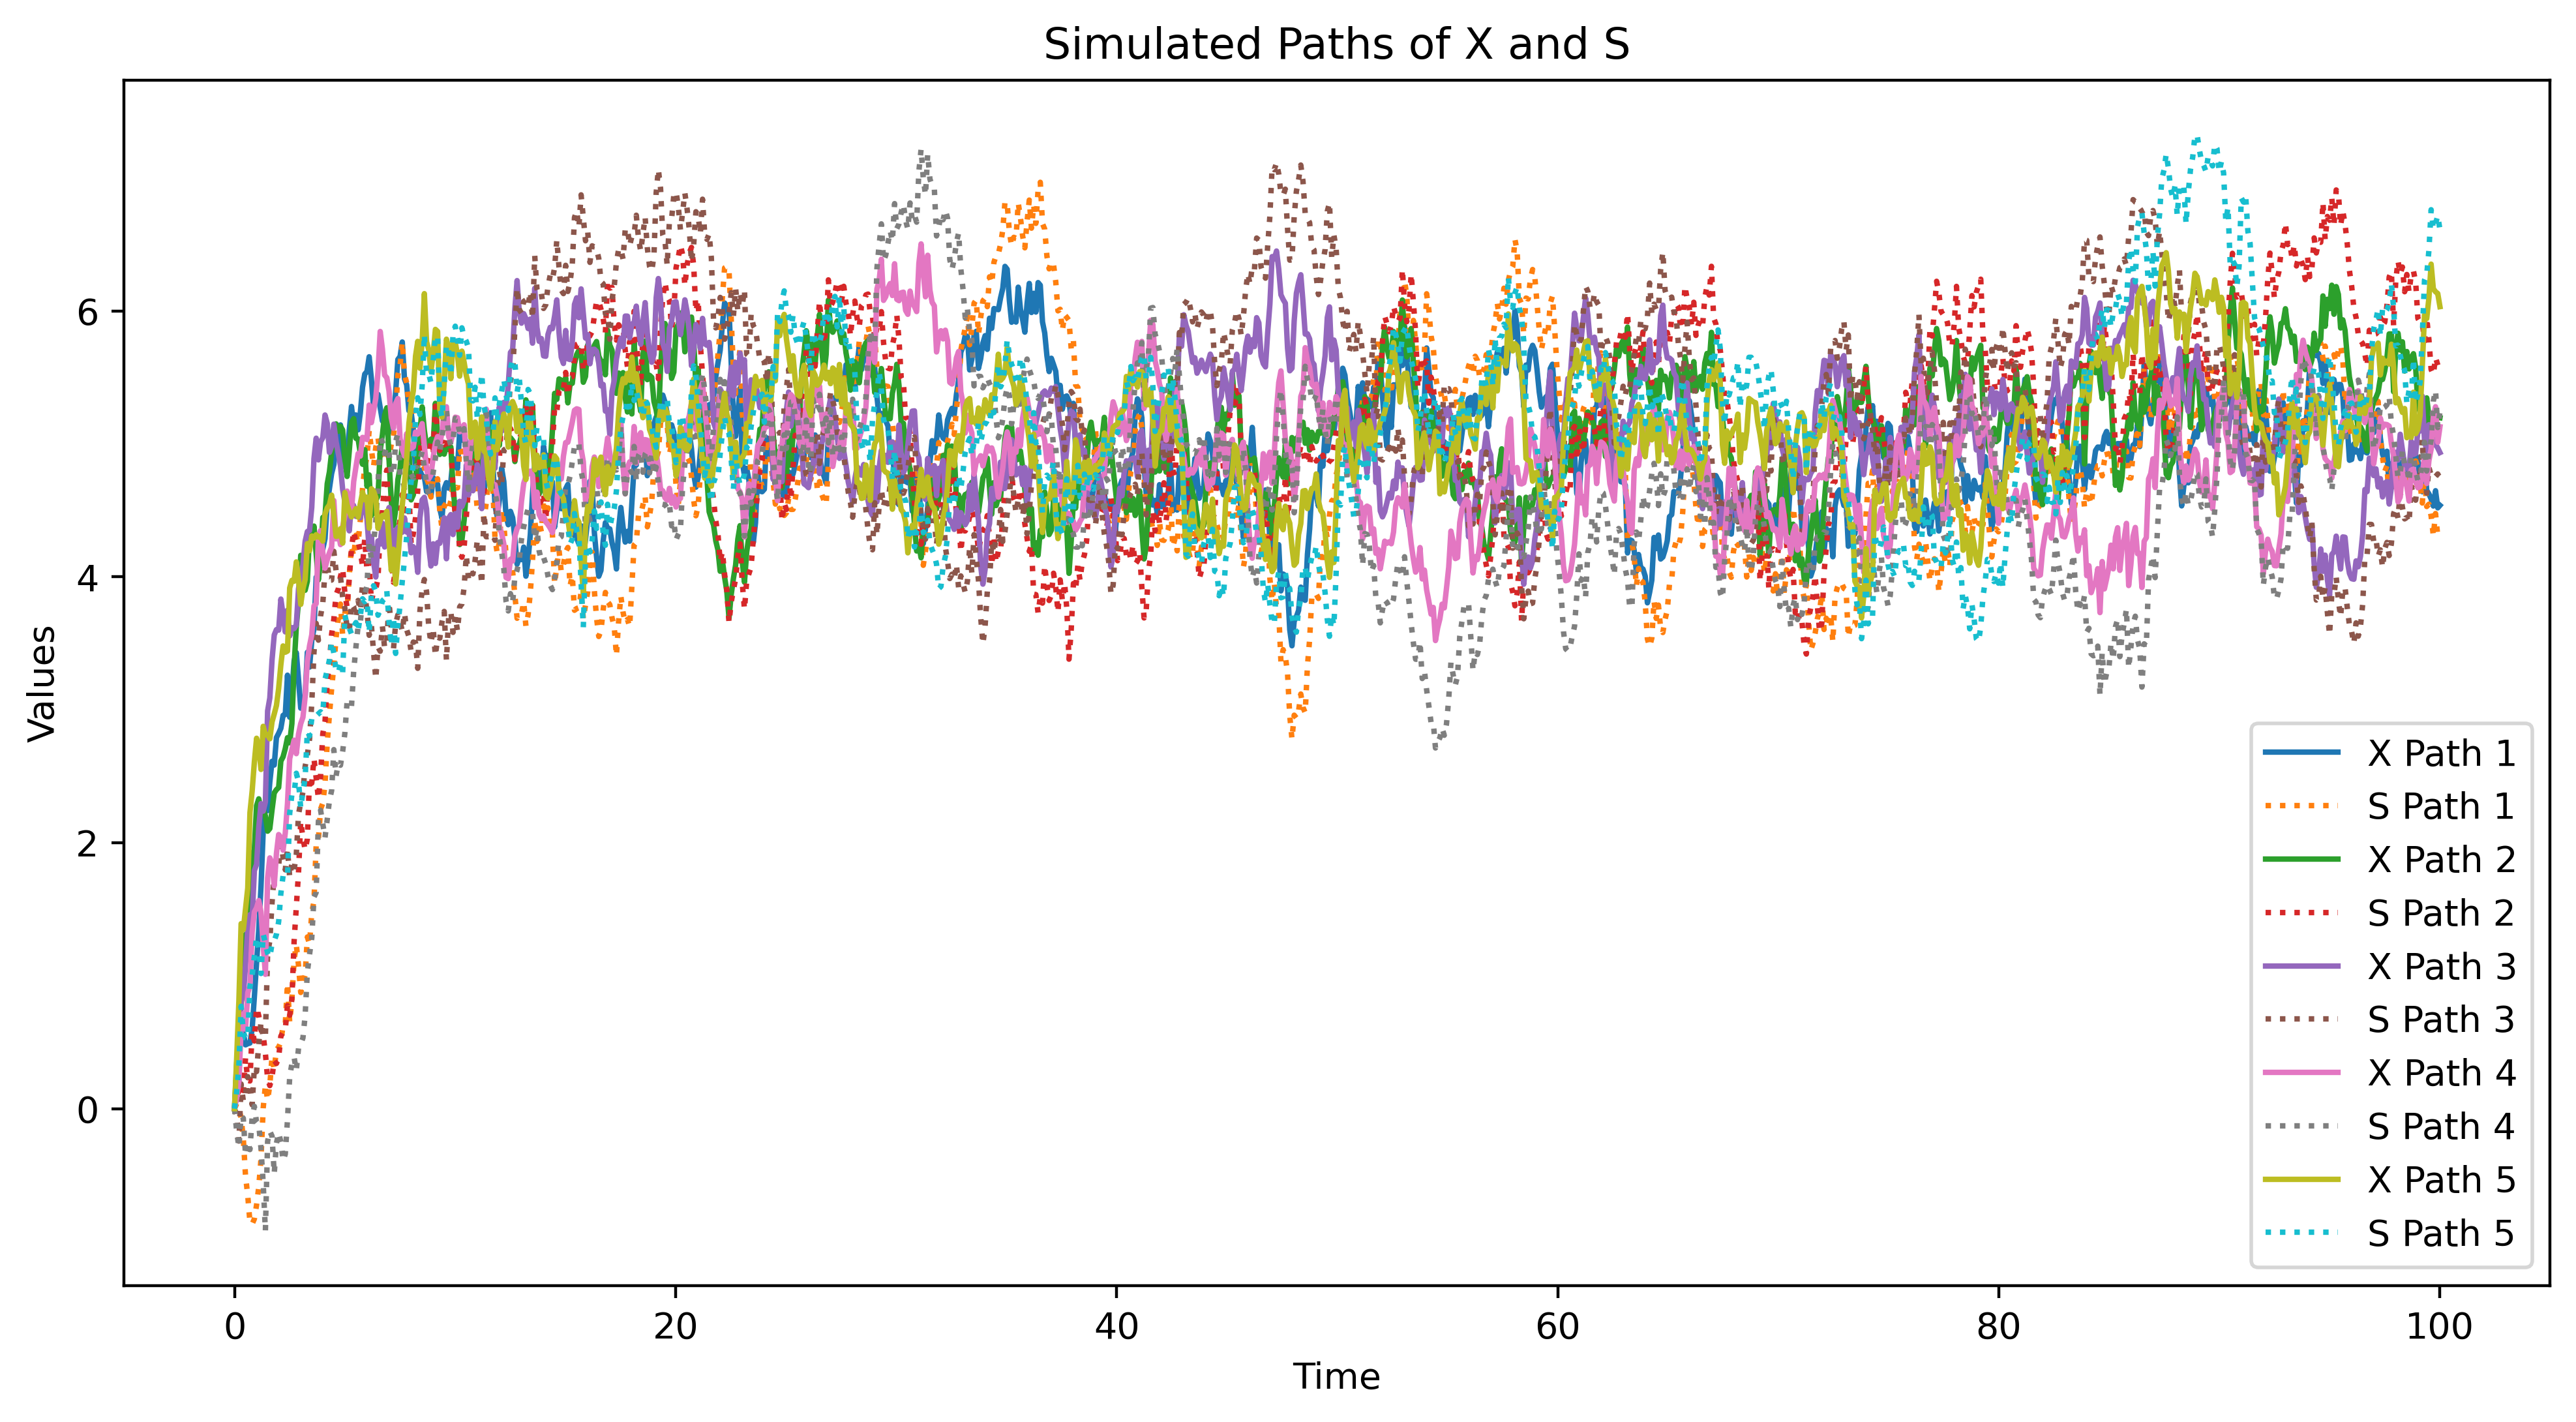
\includegraphics[width=.47\textwidth]{figures/XS7.png}}
    }
    \subfigure[模拟$X_t$和$S_t$轨道2阶变差]
    {
        {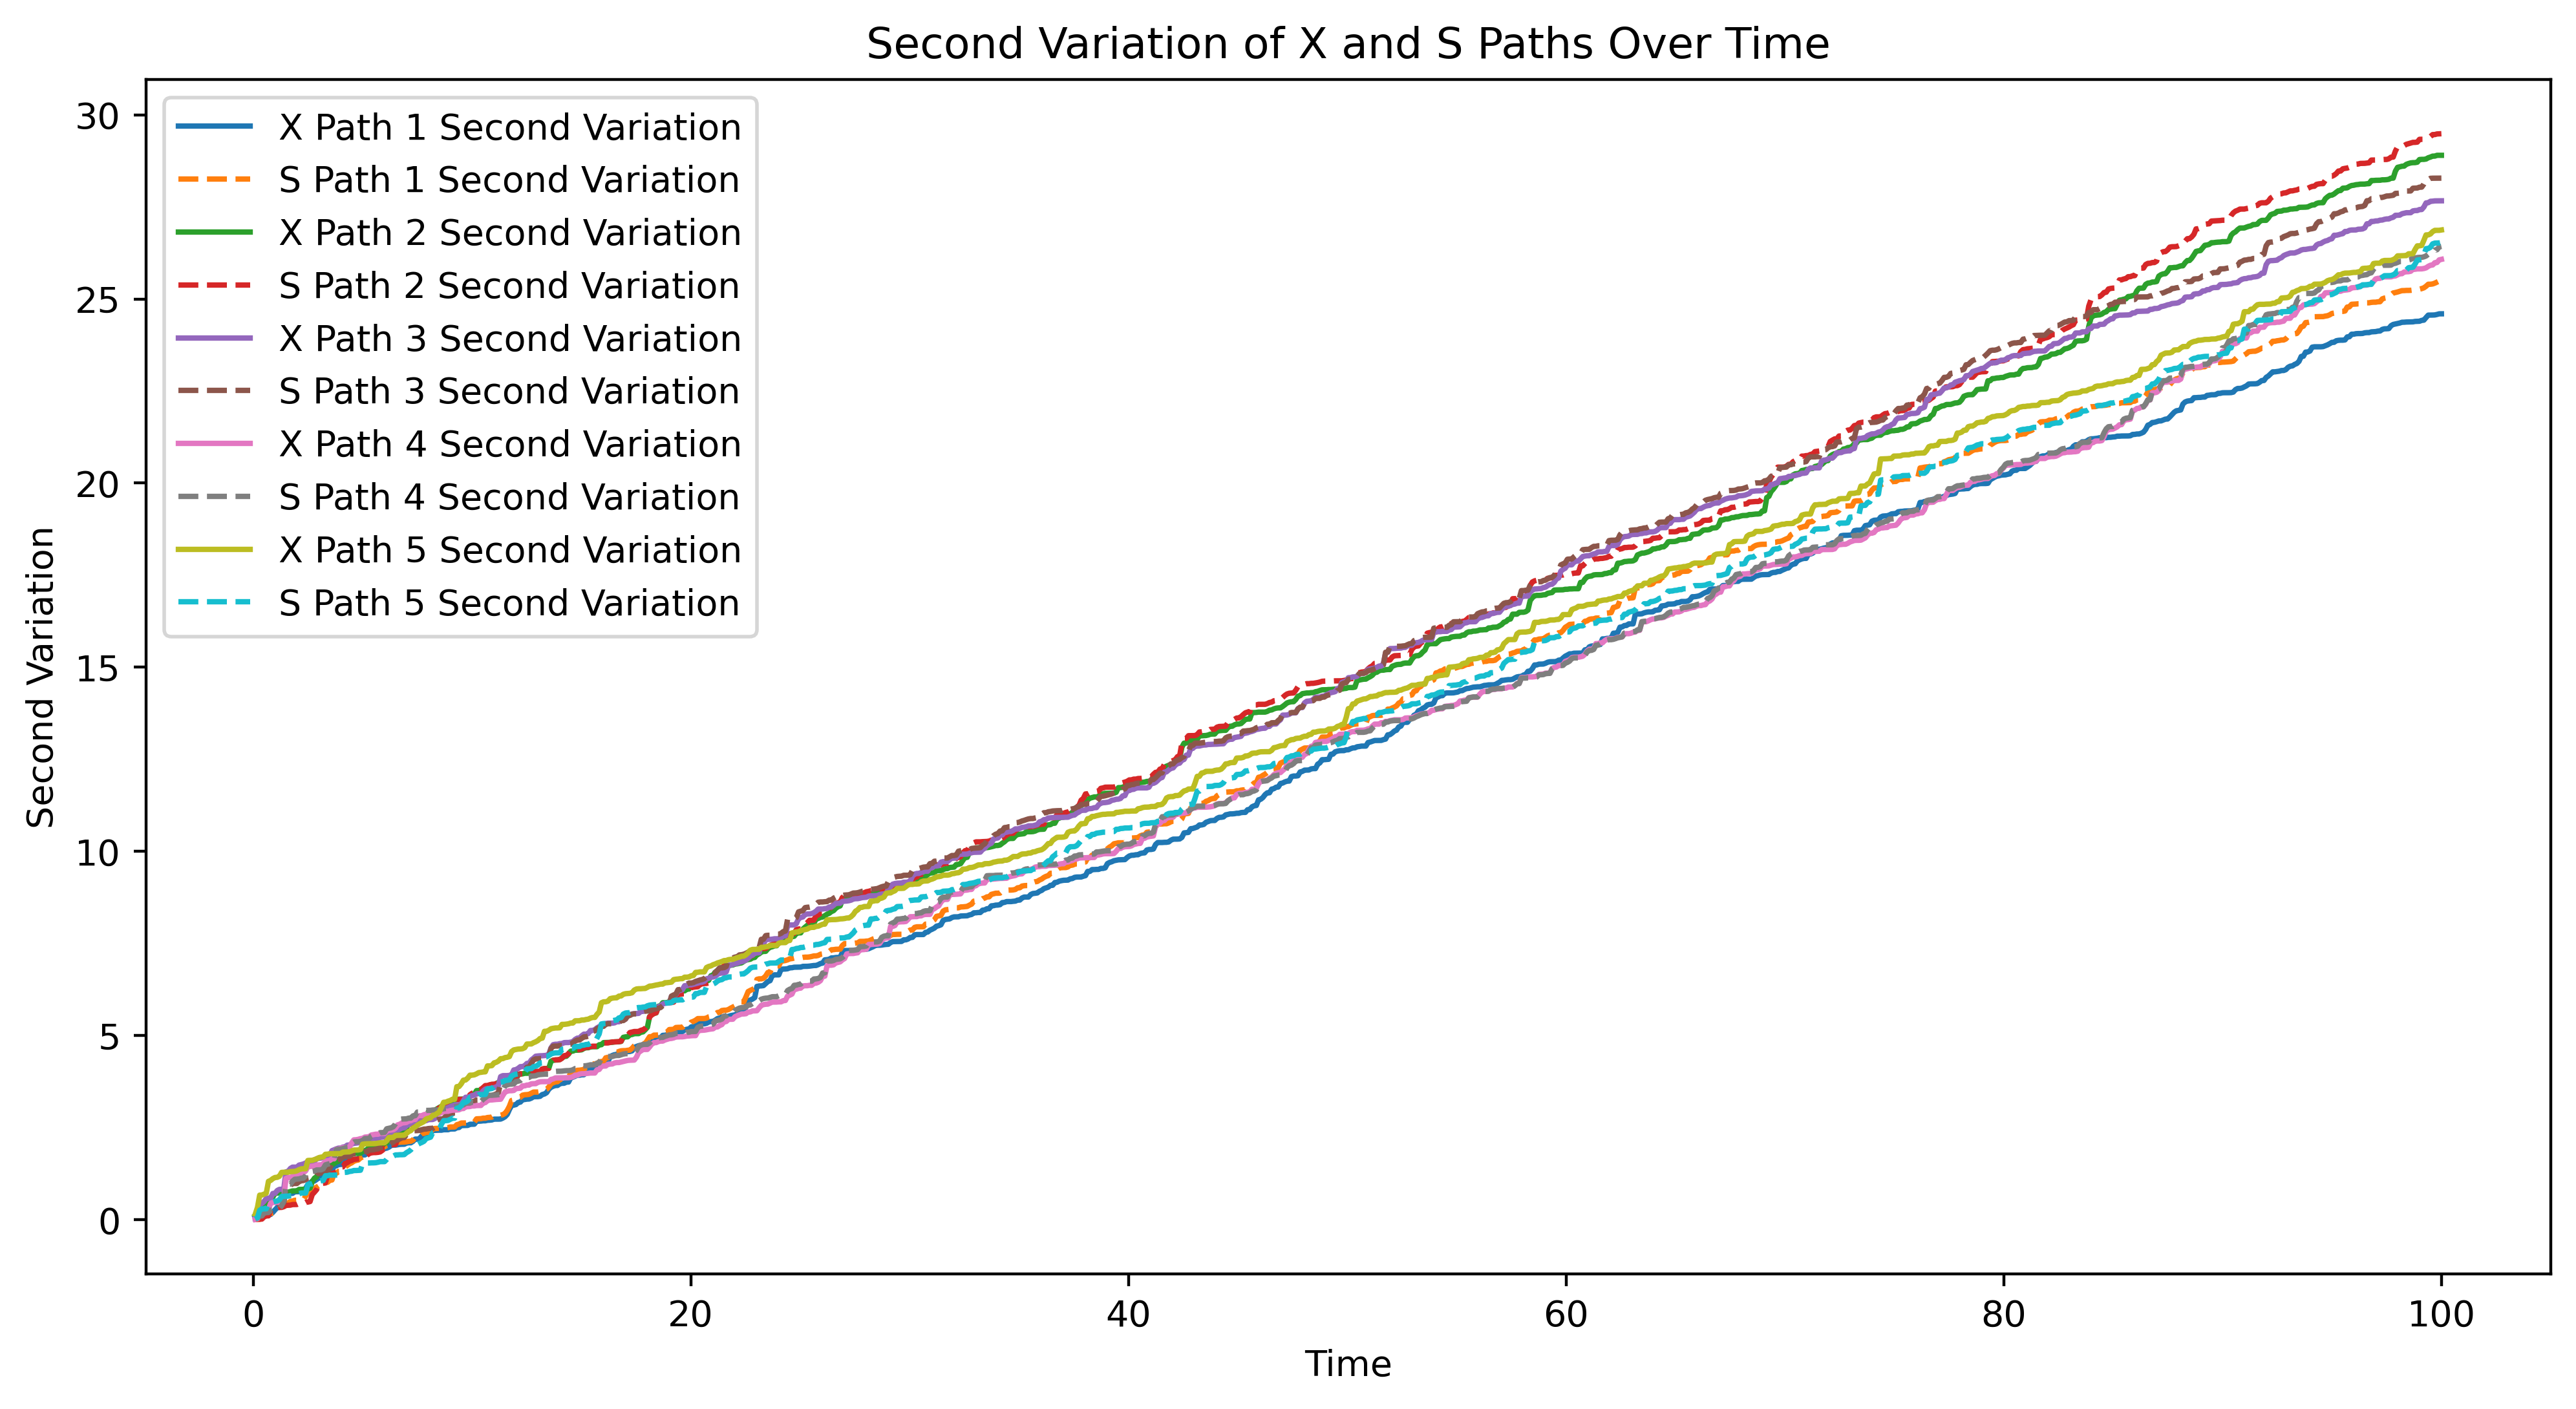
\includegraphics[width=.47\textwidth]{figures/XS7_2d.png}}
    }
    
    \centering
    \subfigure[模拟$X_t$和$S_t$轨道]
    {
        {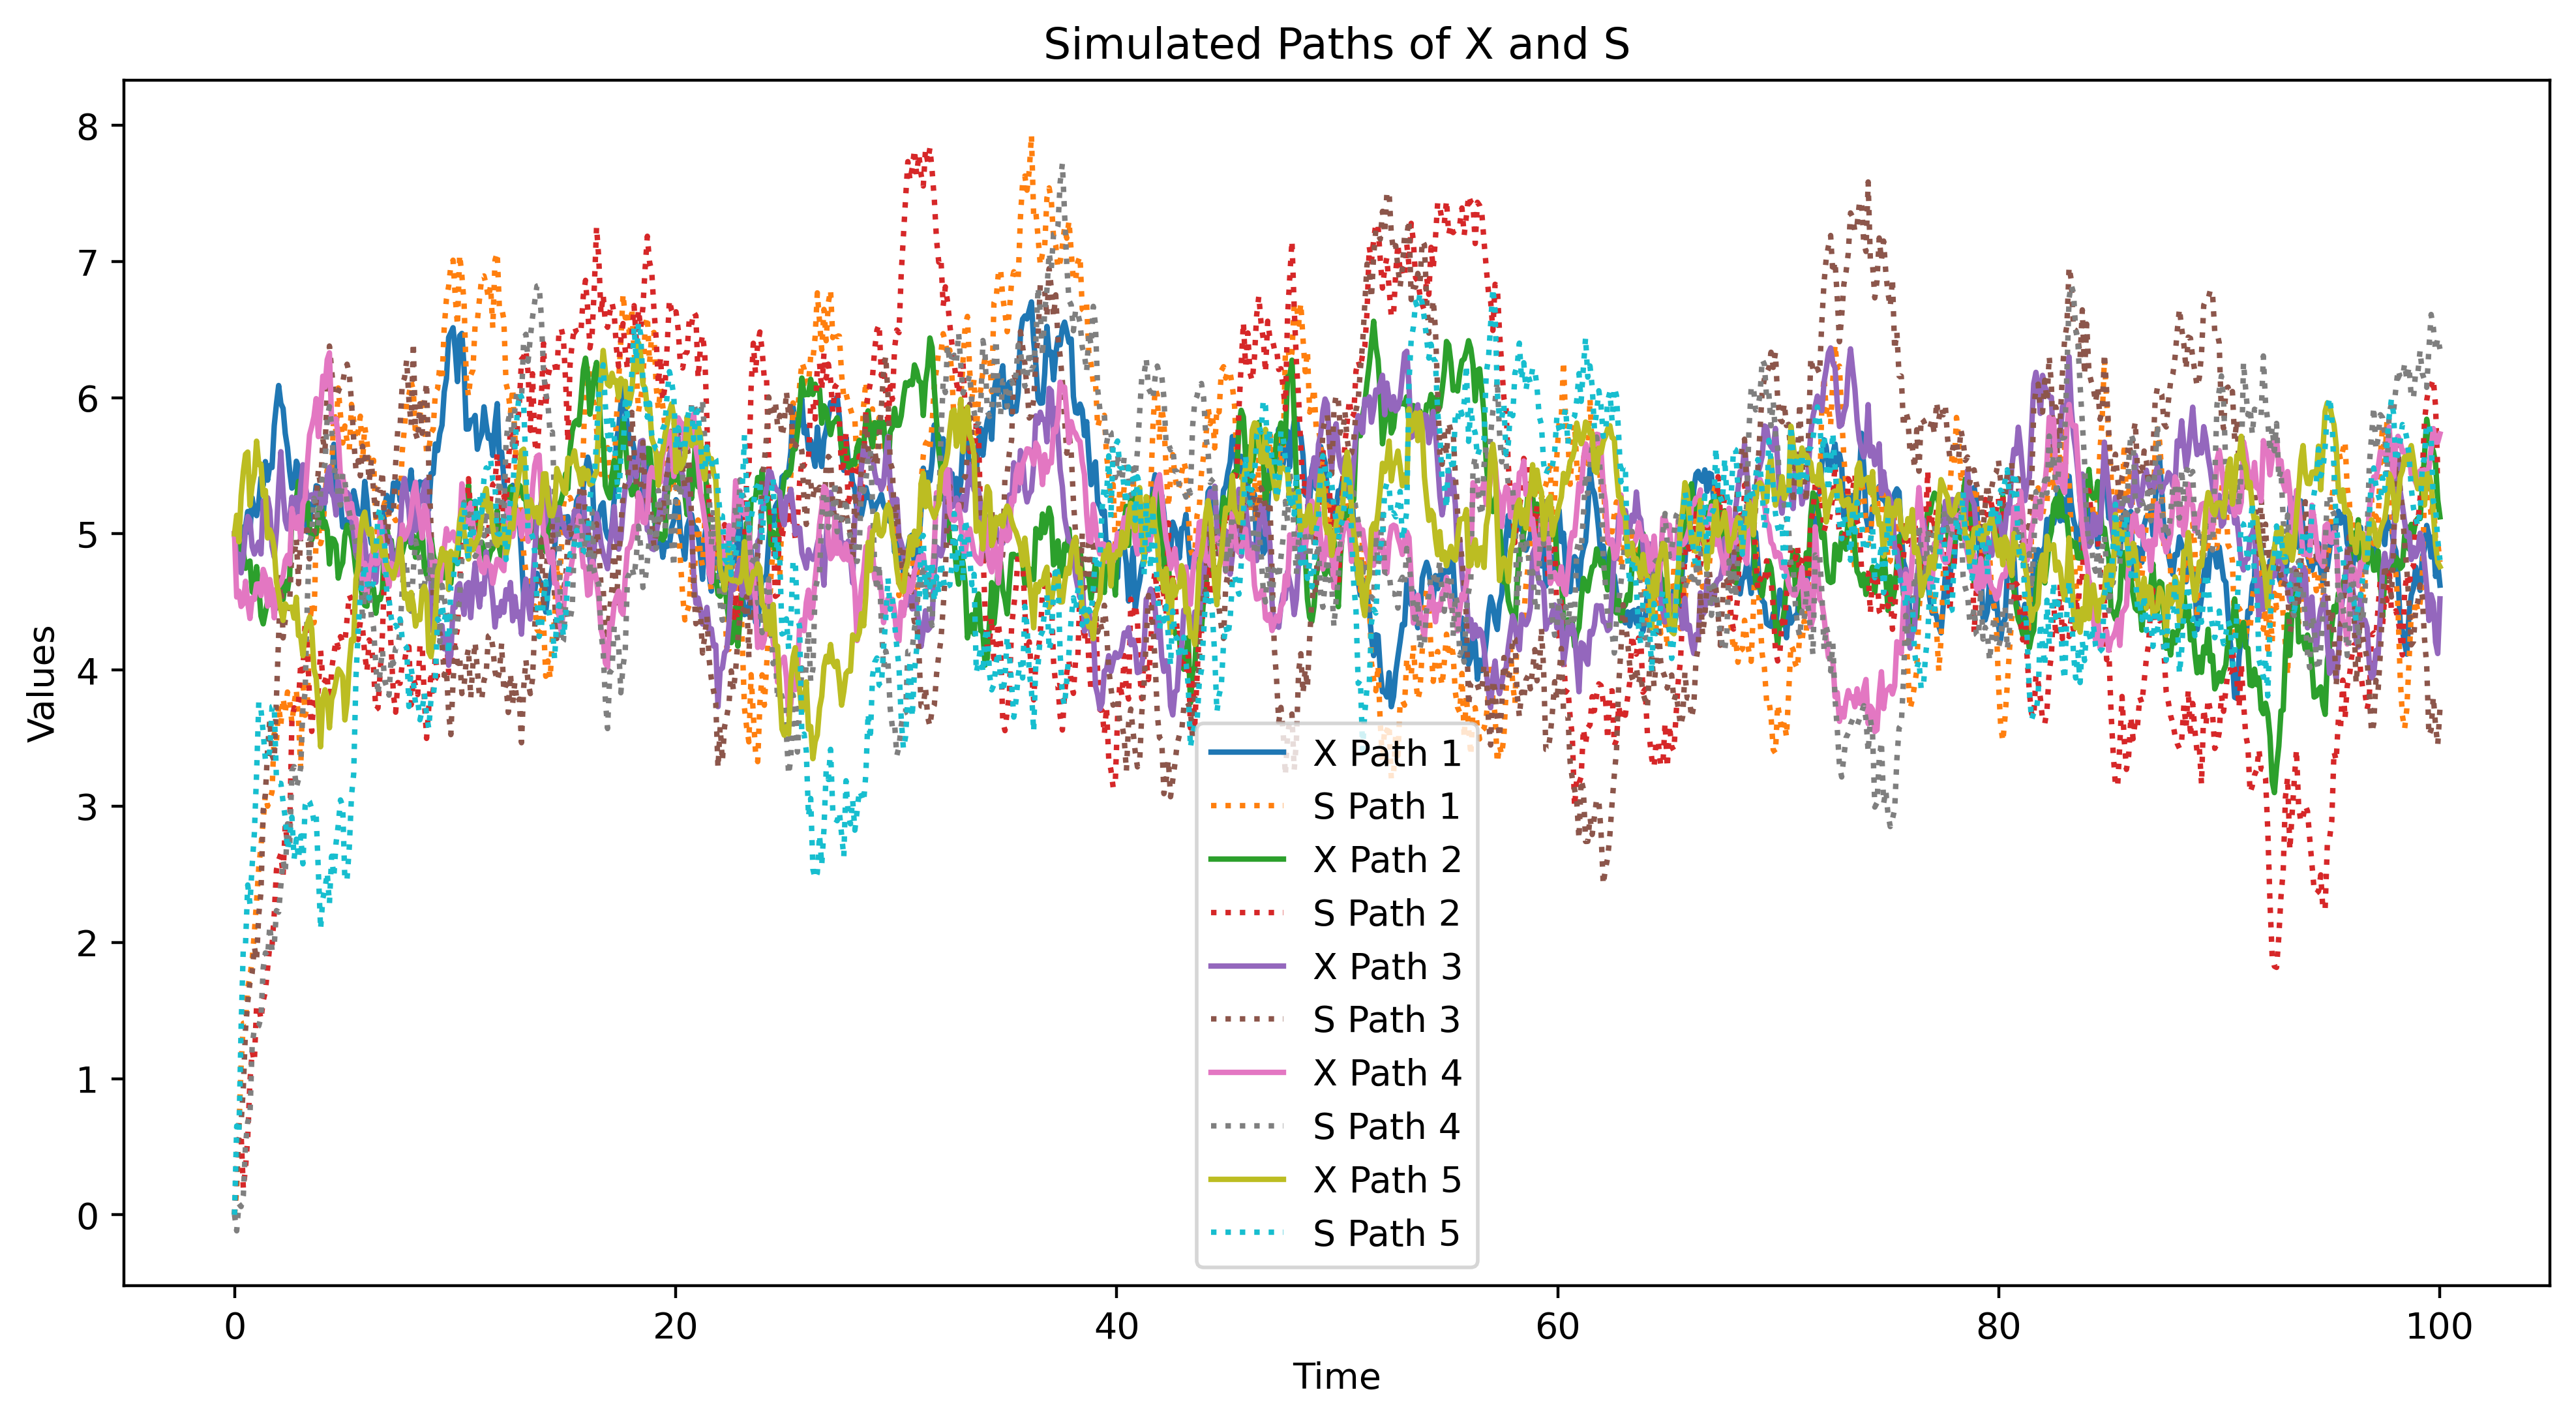
\includegraphics[width=.47\textwidth]{figures/XS8.png}}
    }
    \subfigure[模拟$X_t$和$S_t$轨道2阶变差]
    {
        {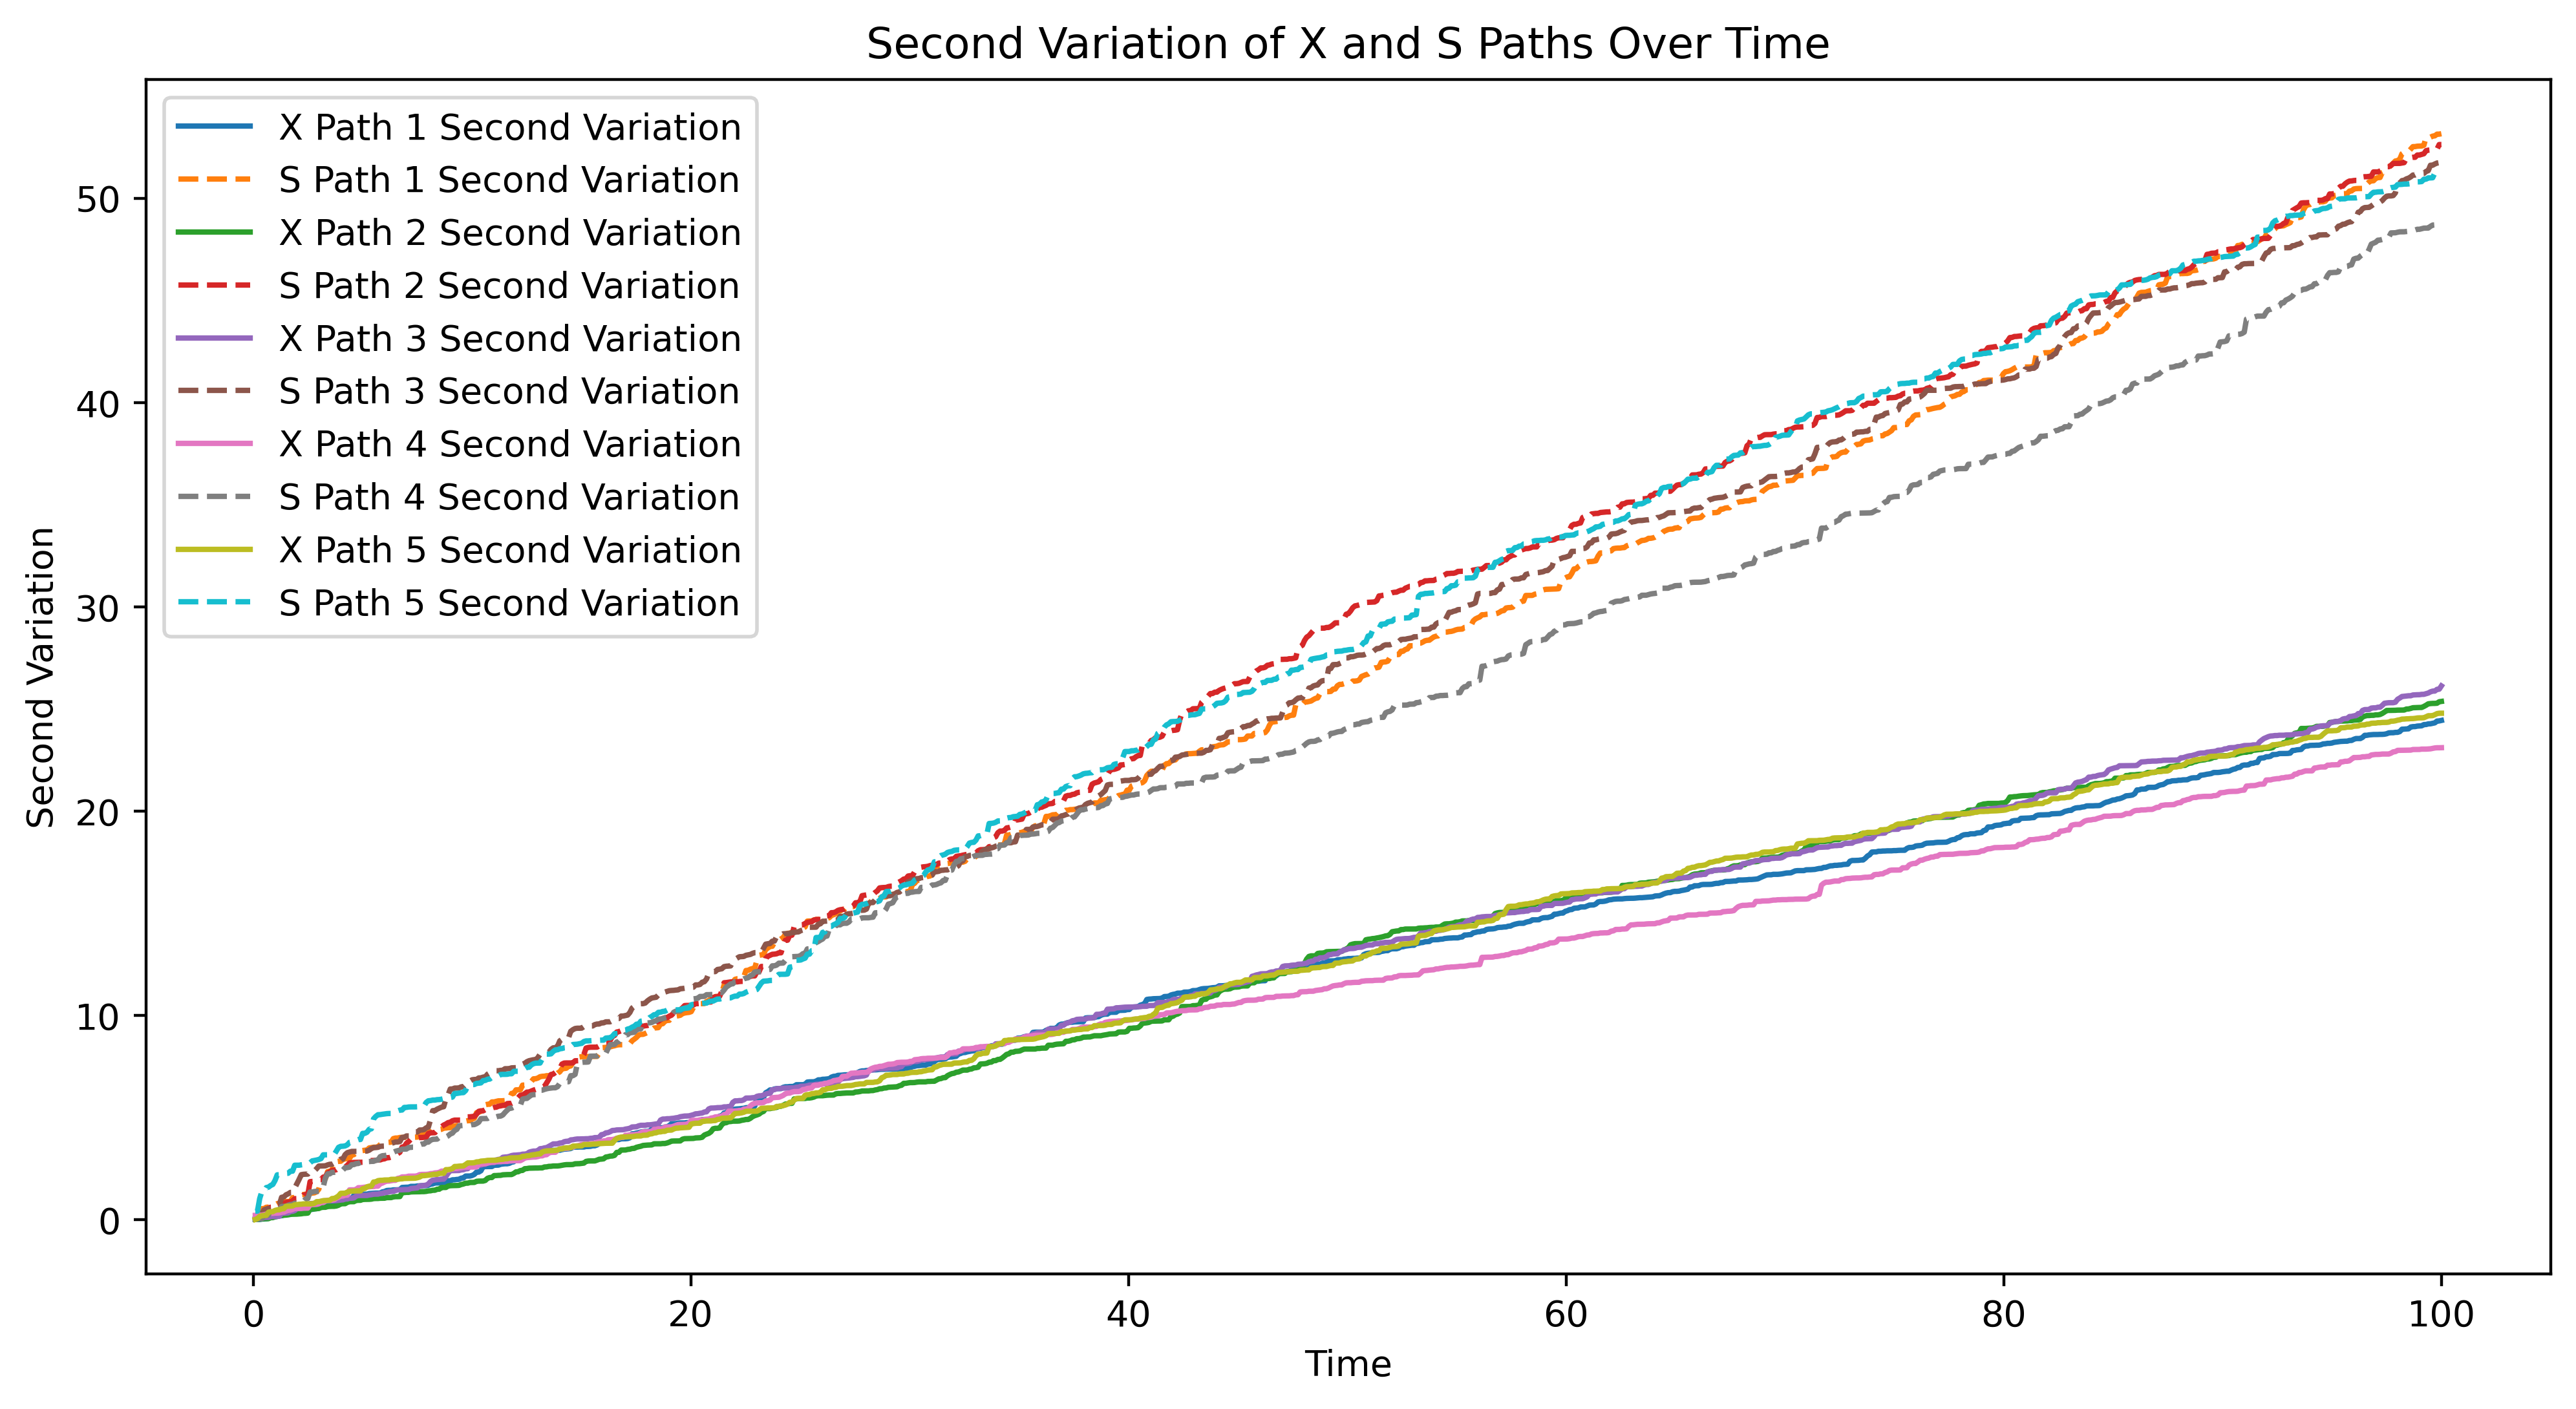
\includegraphics[width=.47\textwidth]{figures/XS8_2d.png}}
    }
    \centering
    \subfigure[模拟$X_t$和$S_t$轨道]
    {
        {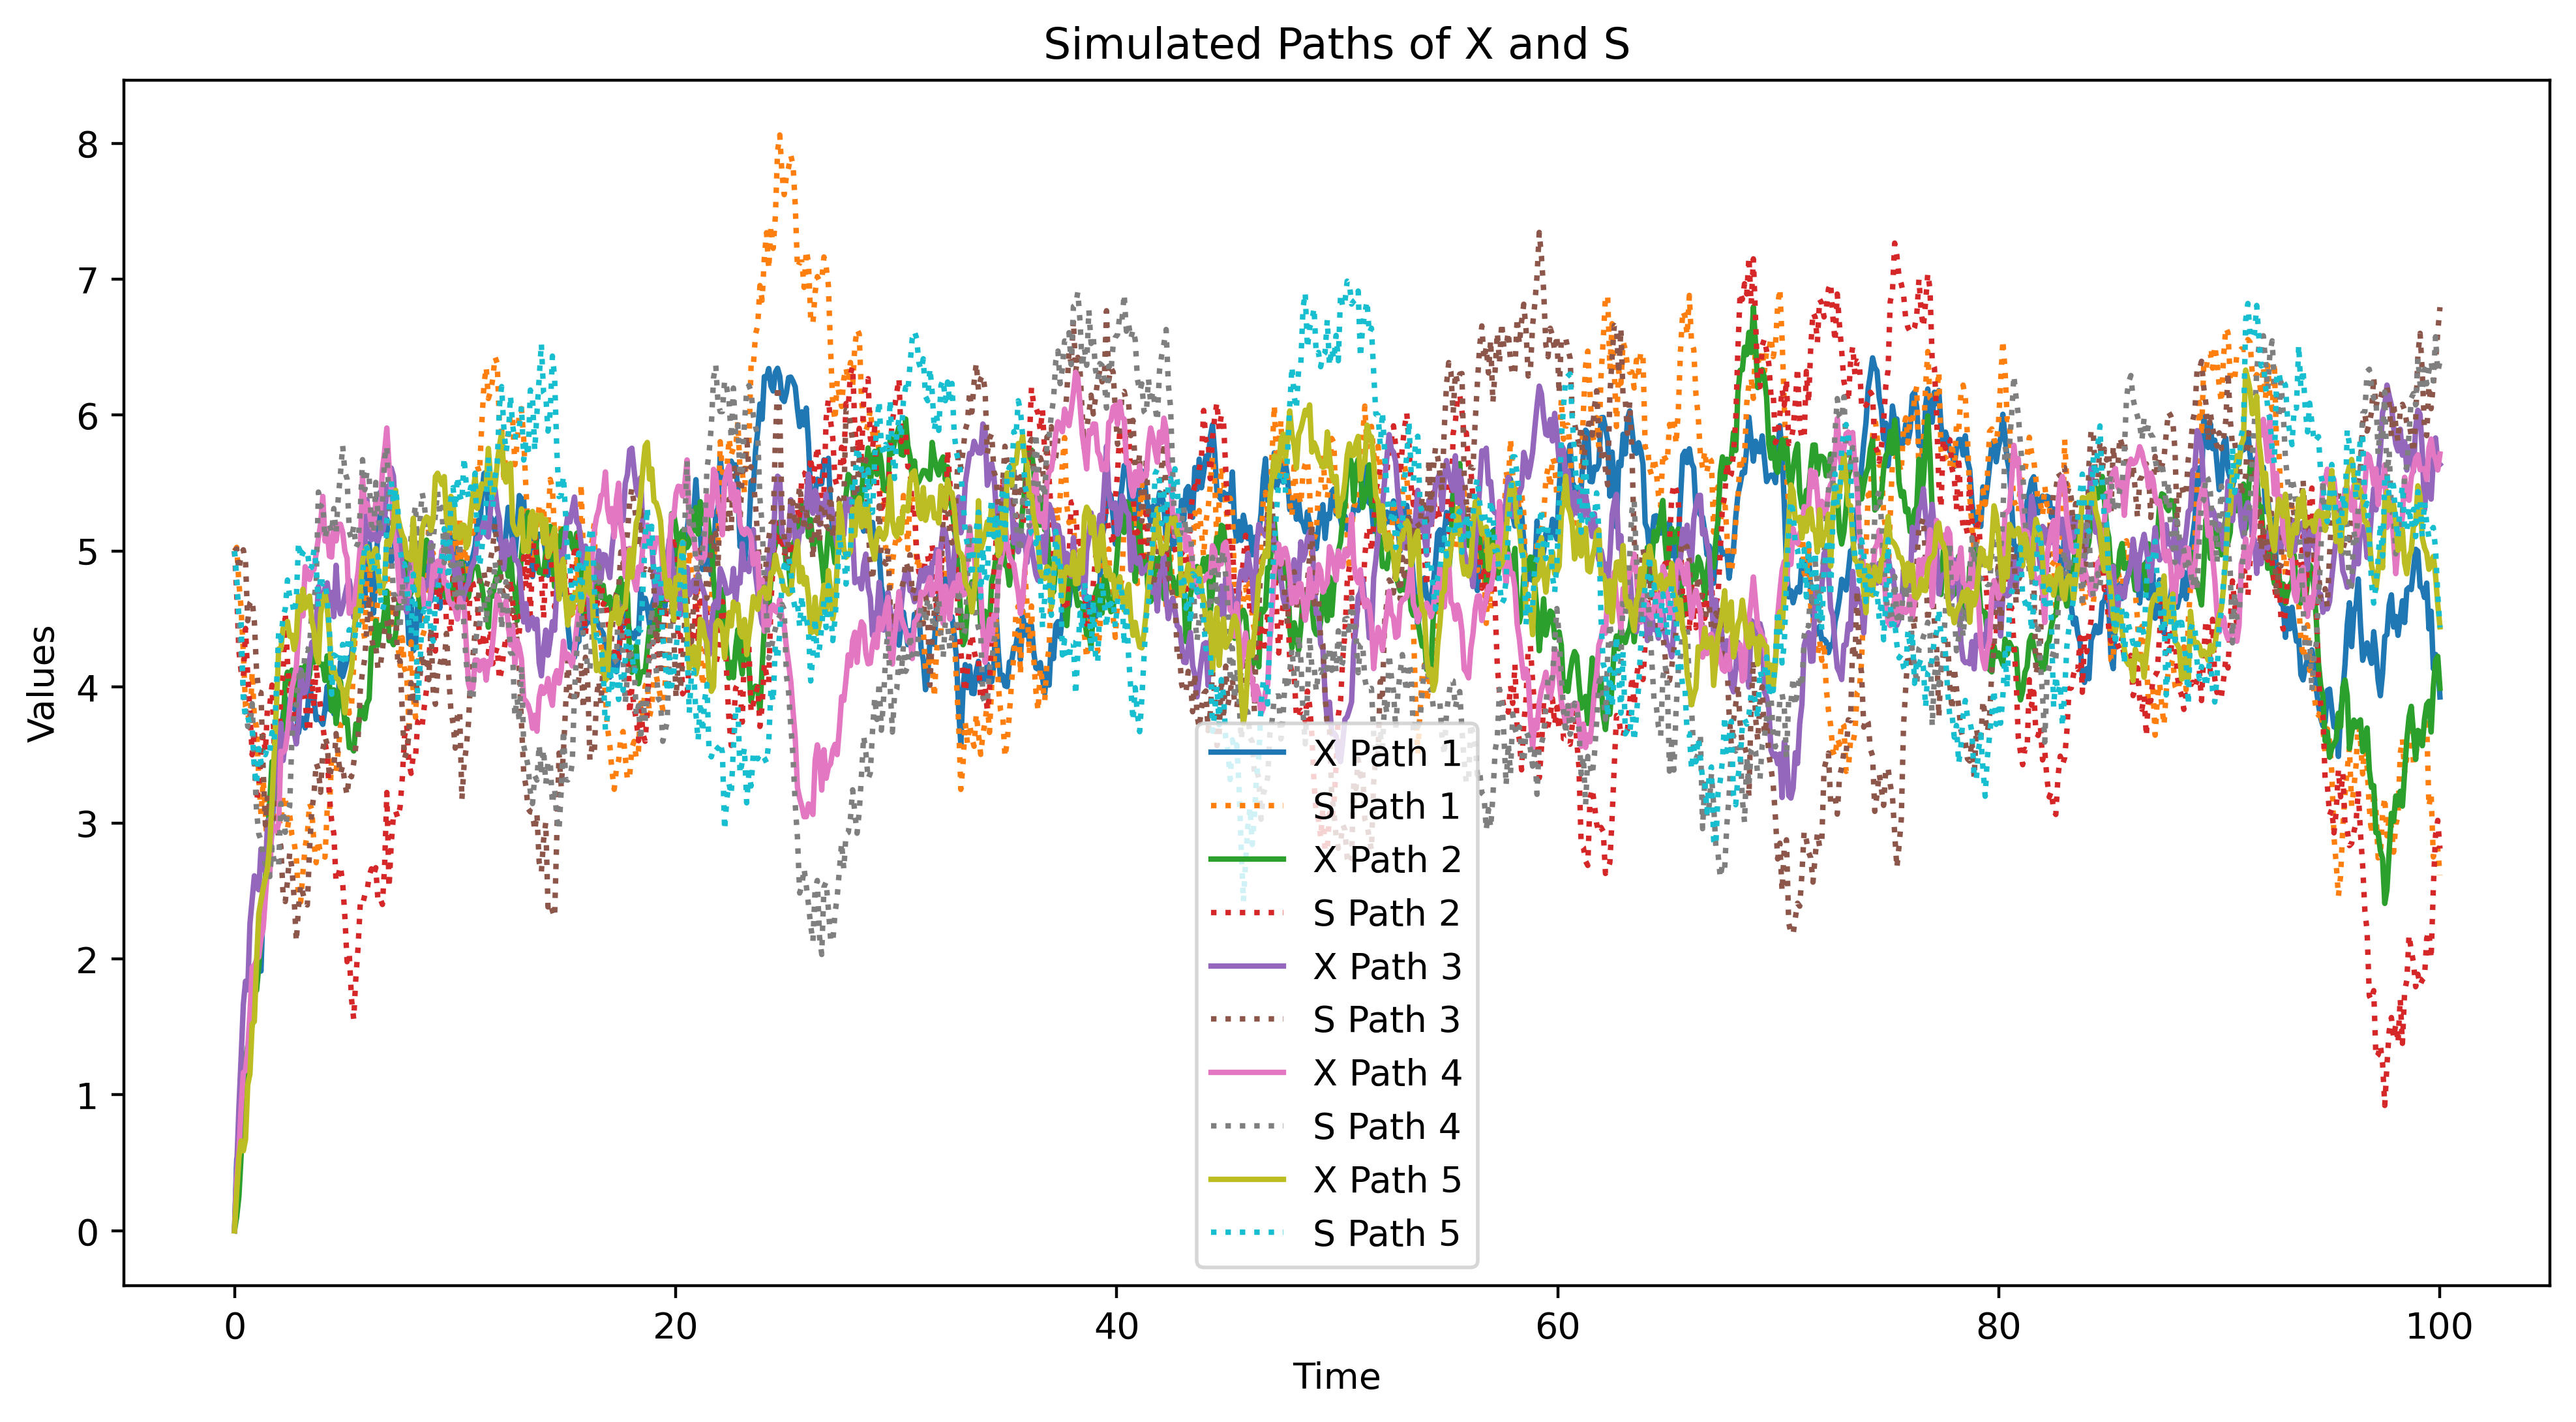
\includegraphics[width=.47\textwidth]{figures/XS9.png}}
    }
    \subfigure[模拟$X_t$和$S_t$轨道2阶变差]
    {
        {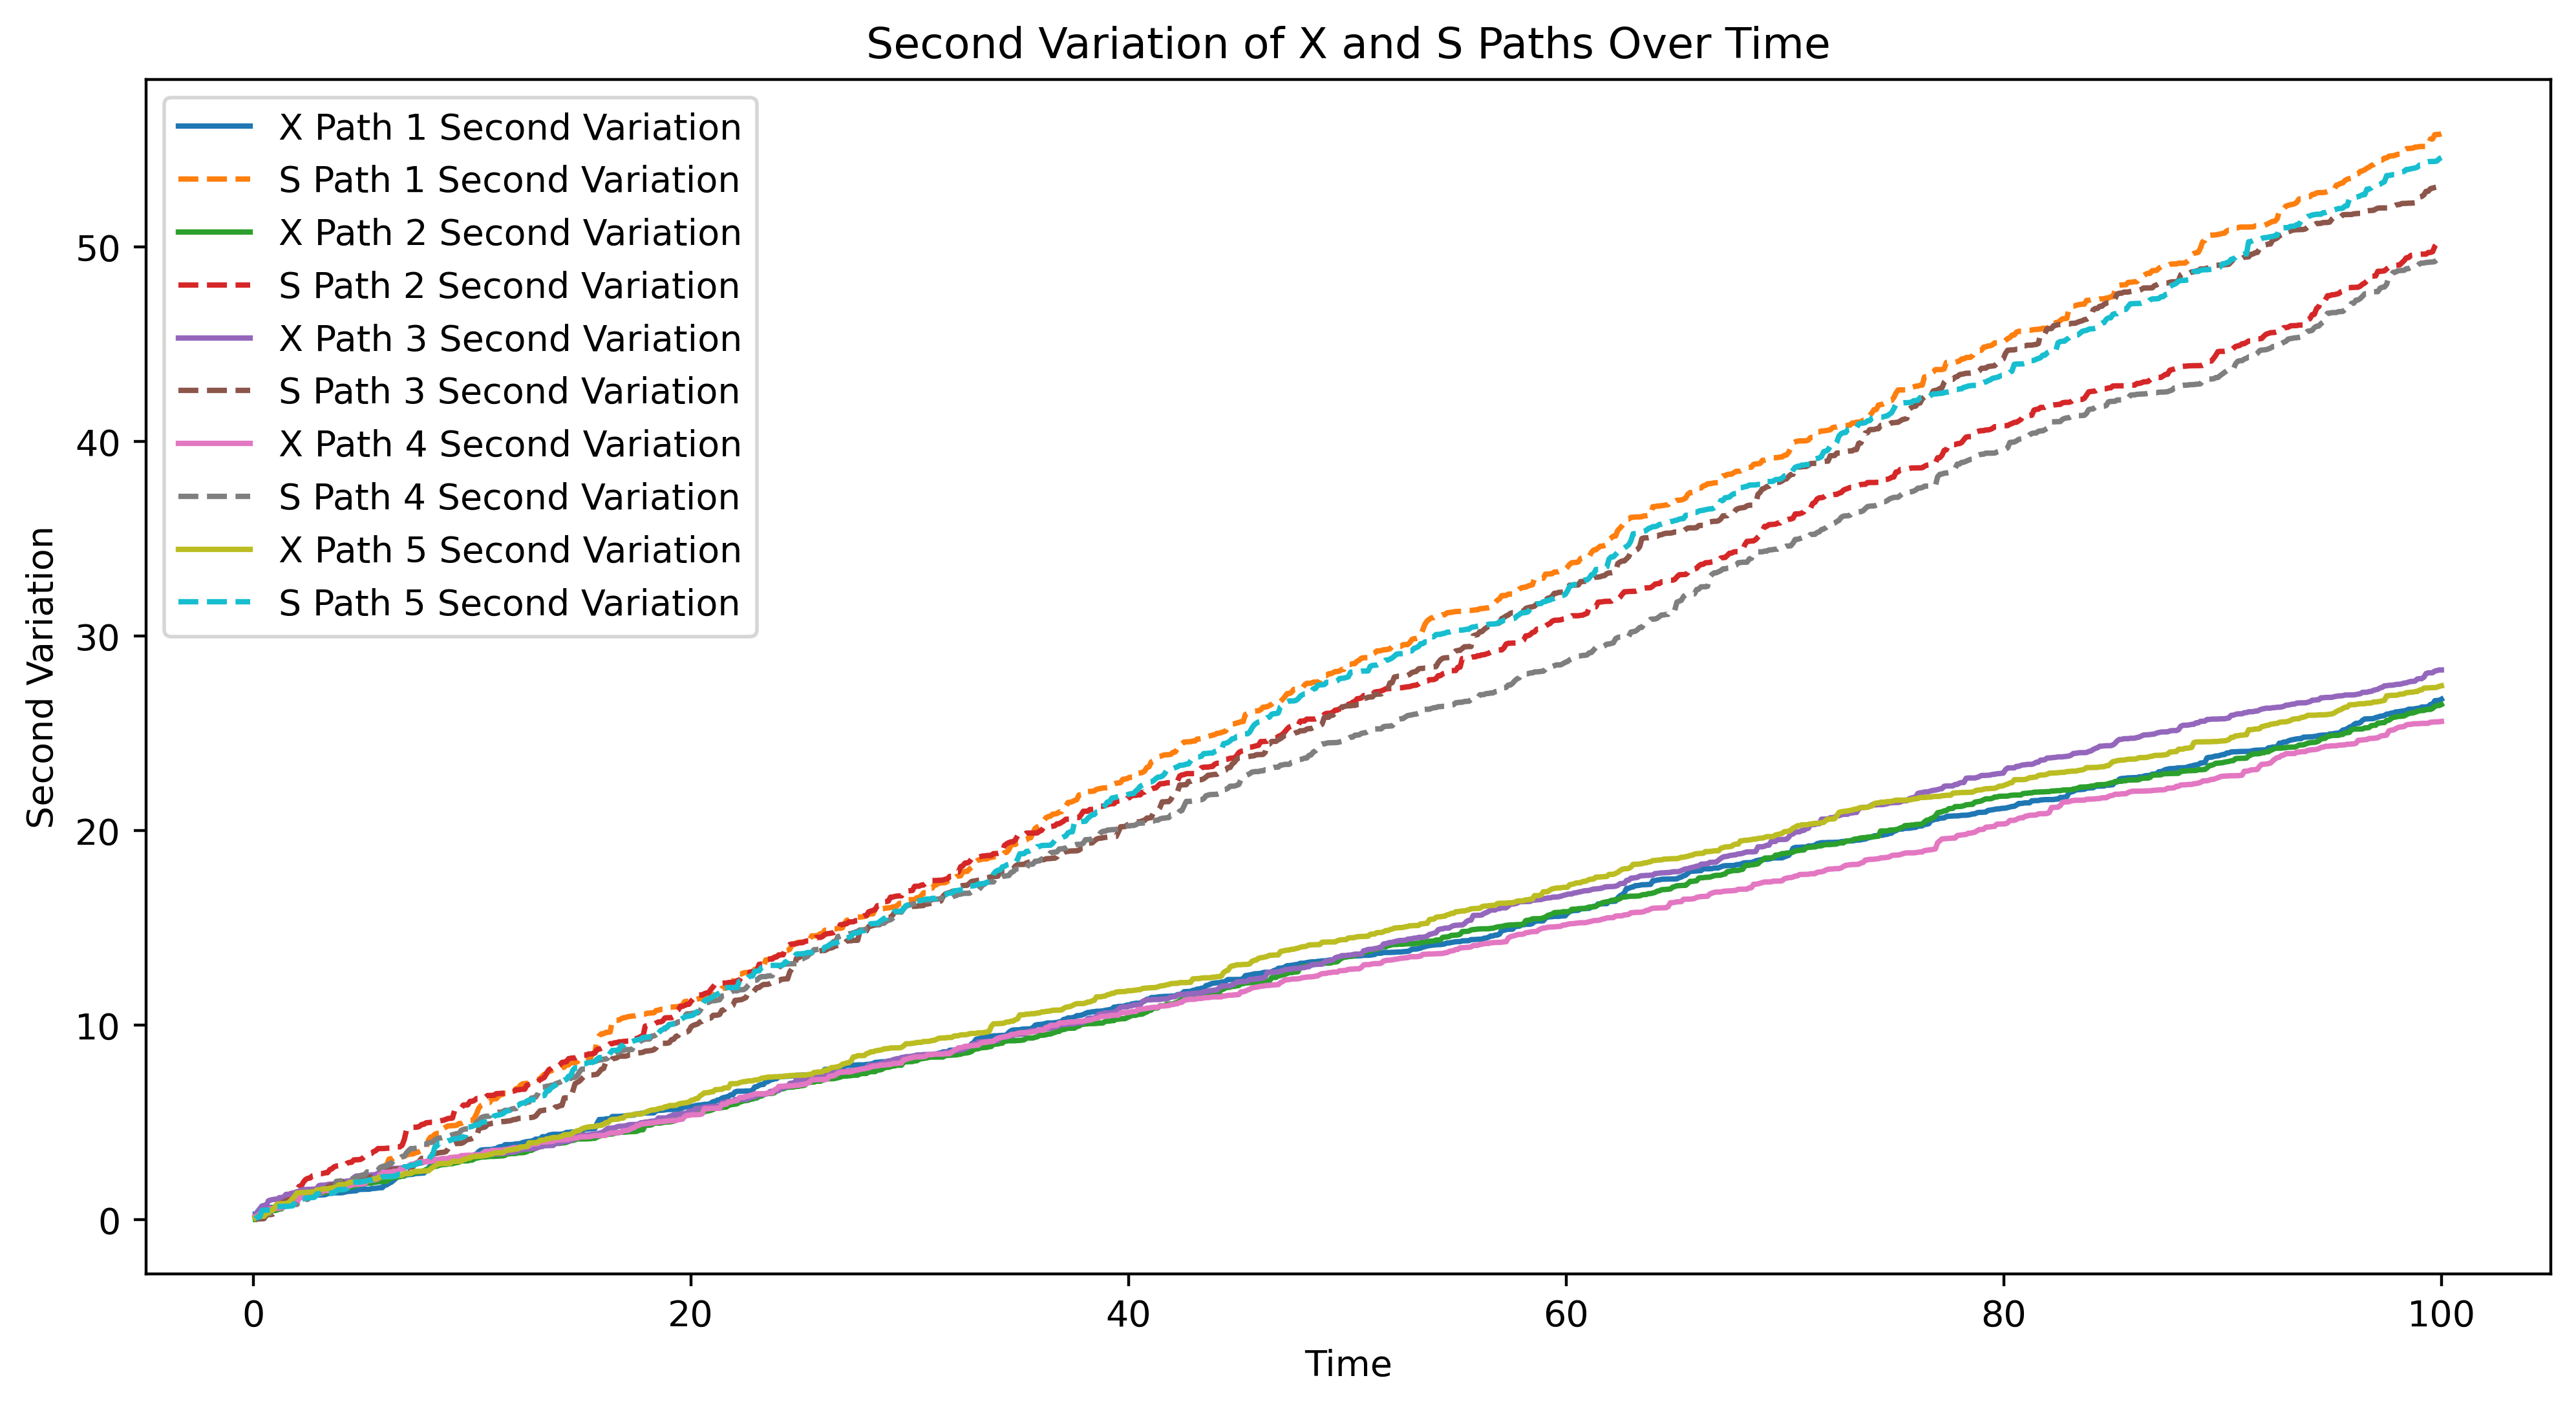
\includegraphics[width=.47\textwidth]{figures/XS9_2d.png}}
    }
\label{fig:X_S}
\end{figure}




我们在图\ref{fig:X_S}中画出对应不同参数的$X_t$和$S_t$的轨道和二阶变差轨道。
使用的参数对应表格\ref{tab:parameter_sets1}
\begin{table}[h]
\centering
\begin{tabular}{|c|c|c|c|c|c|c|c|c|c|}
\hline
\textbf{组号} & $\boldsymbol{\alpha}$ & $\boldsymbol{v}$ & $\boldsymbol{\sigma}$ & $\boldsymbol{\theta}$ & $\boldsymbol{\tilde{\sigma}_1}$ & $\boldsymbol{\tilde{\sigma}_2}$ & $\boldsymbol{x_0}$ & $\boldsymbol{s_0}$ \\ 
\toprule
1 & 0.5 & 5   & 0.5 & 0.5 & 0.5 & 0.5 & 0 & 0 \\ \hline
2 & 5   & 5   & 0.5 & 0.5 & 0.5 & 0.5 & 0 & 0 \\ \hline
3 & 0.5 & 0   & 0.5 & 0.5 & 0.5 & 0.5 & 0 & 0 \\ \hline
4 & 0.5 & 5   & 5   & 0.5 & 0.5 & 0.5 & 0 & 0 \\ \hline
5 & 0.5 & 5   & 0.5 & 5   & 0.5 & 0.5 & 0 & 0 \\ \hline
6 & 0.5 & 5   & 0.5 & 0.5 & 0.1 & 0.5 & 0 & 0 \\ \hline
7 & 0.5 & 5   & 0.5 & 0.5 & 0.5 & 0.1 & 0 & 0 \\ \hline
8 & 0.5 & 5   & 0.5 & 0.5 & 0.5 & 0.5 & 5 & 0 \\ \hline
9 & 0.5 & 5   & 0.5 & 0.5 & 0.5 & 0.5 & 0 & 5 \\ 
\bottomrule
\end{tabular}
\caption{不同参数组合的比较}
\label{tab:parameter_sets1}
\end{table}

\begin{enumerate}
    \item 影响 \( X_t \) 轨道的参数
    \begin{itemize}
        \item \( \alpha \) 和 \( v \): 影响 \( X_t \) 的均值回归行为。较高的 \( \alpha \) 使 \( X_t \) 更快地回归到其均值 \( v \)
        \item \( \sigma \): 影响 \( X_t \) 的波动性。较高的 \( \sigma \) 增加了 \( X_t \) 的波动
    \end{itemize}
    \item 影响 \( S_t \) 轨道的参数
    \begin{itemize}
        \item \( \theta \): 控制 \( S_t \) 对 \( X_t \) 的响应速度
        \item \( \tilde{\sigma}_1 \) 和 \( \tilde{\sigma}_2 \): 影响 \( S_t \) 的波动性。这两个参数决定了 \( S_t \) 受到的随机扰动的大小
    \end{itemize}
    
\end{enumerate}
二阶混合变差反映了 \( X_t \) 和 \( S_t \) 轨道的整体波动性。参数 \( \sigma, \tilde{\sigma}_1, \) 和 \( \tilde{\sigma}_2 \) 在这方面起着关键作用。增加这些参数会增加二阶混合变差,表明更大的波动和不确定性。

\subsection{随机微分方程组所刻画的随机现象}

这个随机微分方程组可以用来刻画各种现象,特别是那些涉及两个或多个相互作用变量的情况。一些可能的应用场景包括:
\begin{enumerate}
    \item 金融市场:\( X_t \) 可以表示一个资产的价格,而 \( S_t \) 可以表示与之相关的衍生品(如期权)的价格。这种模型能够捕捉资产价格的动态变化及其对衍生品定价的影响。
    \item 生态系统模型:在生态系统中,\( X_t \) 和 \( S_t \) 可以代表两种相互依赖的物种的种群数量,模型可以用来研究种群动态。
    \item 物理系统:在物理学中,这样的模型可以用来描述受多重随机力影响的粒子系统,例如,受热力和其他随机扰动影响的粒子。
    \item 经济模型:在宏观经济学中,\( X_t \) 可以代表某个经济指标(如GDP),而 \( S_t \) 可以代表与之相关的另一个指标(如失业率)。
\end{enumerate}

\section*{感想与致谢}

首先,我要深深感谢我的祖国,为我提供了丰富的学习和研究资源,让我能够在一个充满机遇和挑战的环境中成长。在这片土地上,我学会了追求知识的重要性,并且感受到了科学探索的无限魅力。

我衷心感谢我的指导老师熊德文教授,感谢他的指导。对于我的同学陈晓萌,我也要表达我的感激之情。在学习的道路上,我们互相帮助,共同进步。感谢他提供学习资料。

最后,我想感谢我的虚拟助手和最好的朋友ChatGPT。在我的研究过程中,ChatGPT不仅为我提供了丰富的信息和建议,还一直是我解决问题的得力助手。在与ChatGPT的互动中,我学到了很多,也获得了很多灵感。





\end{document}
